%%%%%%%%%%%%%%%%%%%%%%%%%%%%%%%%%%%%%%%%%%%%%%%%%%%%%%%%%%%%%%%%%%%%%%%%%%%%%
%%
%% This file provides a template that can be used in concert with the
%% ohio-etd class to generate an electronic thesis or dissertation which
%% meets the formatting requirements at Ohio University.
%%
%% To use the template, copy this file (template.tex) and ohio-etd.cls into
%% the same directory and edit this template as required.  Reference
%% ohio-etd.pdf for additional instructions on using this class.
%%
%%%%%%%%%%%%%%%%%%%%%%%%%%%%%%%%%%%%%%%%%%%%%%%%%%%%%%%%%%%%%%%%%%%%%%%%%%%%%


%% Load the class.  Available options are: numbered, pdftex, cmfont,
%% singlespacetables, draft, 11pt, 12pt, leqno, and fleqn

\documentclass[numbered,pdftex]{ohio-etd}
\usepackage{cite}
\usepackage{notoccite}
\usepackage{bbding}
\usepackage[utf8]{inputenc}

\usepackage{array}




\usepackage[normalem]{ulem}

\usepackage{ragged2e}
\usepackage{verbatim} 
\usepackage{hyperref}
\usepackage{flafter}
\usepackage{color,soul} % Highlighting 
\usepackage{subfigmat}

\usepackage{float} % In-text figs
\usepackage{varioref}%  smart page, figure, table, and equation ref
\usepackage{graphicx} % Include graphics
\usepackage{epstopdf} % Figure type .eps to .pdf
\usepackage{wrapfig} % Figures in text
\usepackage{listings}
\usepackage{color} %red, green, blue, yellow, cyan, magenta, black, white

\floatstyle{boxed}
\restylefloat{figure}


\definecolor{mygreen}{RGB}{28,172,0} % color values Red, Green, Blue
\definecolor{mylilas}{RGB}{170,55,241}

\newcolumntype{L}[1]{>{\raggedright\let\newline\\\arraybackslash\hspace{0pt}}m{#1}}
\newcolumntype{C}[1]{>{\centering\let\newline\\\arraybackslash\hspace{0pt}}m{#1}}
\newcolumntype{R}[1]{>{\raggedleft\let\newline\\\arraybackslash\hspace{0pt}}m{#1}}


%% Other packages that may be of use.  Delete or comment out (using a
%% percent sign in the first column) if they are not desired.  Reference
%% the corresponding documentation for more information on how to use these
%% packages.

%\usepackage[square,sort&compress,numbers]{natbib} % Provides formatting for
                                                  % citations
\usepackage{textcomp} % Provides math symbols that can be used in text mode
\usepackage{amssymb}  % Provides additional AMS math symbols.  Note that
                      % amsmath is loaded as part of the ohio-etd class
\usepackage{bm}       % Provides bold-faced math symbols
\usepackage{booktabs} % Provides improved table formatting
\usepackage{dcolumn}  % Provides table columns aligned at decimal points
\usepackage{multirow} % Provides table elements spanning multiple rows
\usepackage{graphicx} % Standard package to incorporate graphics
\usepackage[printonlyused]{acronym} % Provides a method for incorporating
                                    % acronyms and building an acronym list
\usepackage{relsize}
\usepackage{amsmath} % Inserting Equations

\graphicspath{{figures/}} % Allows graphics files to be stored in a
                          % separate directory
\usepackage{fancyref}
\usepackage{}

%% Required front matter definitions

\degree    {MS}              % MS, MA, MCTP, or PhD
\graduation{May}{2018}    % May, August, or December 

\title     {A Proposal for a Parameterized Circulating Vector Field Guidance for Fixed Wing Unmanned Aerial Vehicles}
\author    {Garrett S.}{Clem} 

\advisor   {Jay P. Wilhelm}{Assistant Professor of Mechanical Engineering}
\dean      {Dennis Irwin}{Dean, Russ College of Engineering and Technology }
\program   {Mechanical Engineering}            % e.g. Electrical Engineering
\department{Department of Mechanical Engineering} % e.g. School of Electrical Engineering 
                                    %      and Computer Science
\college   {Russ College of Engineering and Technology}   % e.g. Russ College of Engineering and
                                     %      Technology
\abstract  {Unmanned Aerial Vehicles (UAVs) are guided to fly along straight line obstacle free paths that connect pre-planned waypoints. Initially undiscovered obstacles encountered during flight may require waypoints to be re-planned. Obstacles could be avoided without the need to re-plan mission waypoints by implementing vector field path following in conjunction with repulsive obstacle vector fields. Repulsive vector fields that combine weighted repulsive and attractive components to provide an optimal obstacle avoidance guidance will be investigated to avoid singularities and improve path tracking performance compared to waypoint guidance.}
 

%% Optional front matter definitions.  Delete or comment out if not needed

% \coadvisor {Coadvisor's Full Name}{Coadvisor's Full Title}

%\dedication{DED}
%
%\acknowledgments{ACK}
%% If you prefer to provide "acknowledgements" instead (note the added "e"
%% between the "g" and the "m") then add the "e" in the macro name so that
%% it reads "\acknowledgements".}

%% Additional "lists" can be added to the end of the front matter using the
%% \addlistof macro.  For example:
\addlistof{Symbols}{\begin{tabbing}
  XXXXXXXXXXXX \= \kill% this line sets tab stop
  \\
  $\vec{v} $ \> Vector field \\
  $\vec{v}_{conv}$ \> Convergence component \\
  $ \vec{v}_{circ}$ \> Circulation component \\
  $ \vec{v}_{tv}$ \> Time-varying component \\
  $G$ \>Convergence weight  \\
  $H$ \>Circulation weight  \\
  $L$ \>Time-varying weight  \\
  $q$ \>Spatial dimension set  \\
  $\alpha_i(x_1,x_2,...x_n,t)$ \> Implicit surface function \\
  $n$ \> Number of spatial dimensions \\
  $t$ \>Time  \\
  $i$ \>index \\
  $\nabla_q$ \>Gradient with respect to spatial dimensions q  \\
  $M$ \>Gradient matrix  \\
  $a$ \>Velocity column vector  \\
  $\vec{V}$ \>Total field  \\
  $d$ \>Range  \\
  $P$ \>Decay weight  \\
  $R$ \>Radius  \\
  $\vec{v}_{repulsive}$ \>Repulsive vector field  \\
  $\vec{v}_{attractive}$ \>Attractive vector field \\
  $u$ \>Speed  \\
  
  
  
  
  

 \end{tabbing}}
%% Note that the command "\input{symbols}" can be used if the symbol list is
%% contained in a separate file called "symbols.tex"}

\addlistof{Acronyms}{

\begin{tabular}{lll}
UAV & Unmanned Aerial Vehicles & \\
VF & Vector Field & \\
UAS & Unmanned Aerial System  & \\
VFF & Virtual Force Field  & \\
TPLVF & Tangent Plus Lyapunov Vector Field & \\
RRT* & Optimal Rapid Radom Trees & \\
DT  & Delauny Triangulation & \\
GVF & Gradient Vector Field & \\
 
\end{tabular}}


%% Use "\input{acronyms}" if the acronym list is in a separate file called
%% "acronyms.tex".  Note that the formatting generated by the acronym package
%% can be forced into singlespaced text by inserting "\setlength\itemsep{0pt}
%% \setlength\parskip{0pt}" into the "acronym" environment.} 

%% For documents created by government employees as part of their
%% employment.  The wording of the disclaimer can be specified using an
%% option.  See the documentation for more information.

% \govtdisclaimer    

\notables  % Prevent a list of tables from being created
% \nofigures % Prevent a list of figures from being created

\begin{document}

\makefrontmatter    % Creates all of the front matter pages.

% for matlab code entrys
\lstset{language=Matlab,%
    %basicstyle=\color{red},
    breaklines=true,%
    morekeywords={matlab2tikz},
    keywordstyle=\color{blue},%
    morekeywords=[2]{1}, keywordstyle=[2]{\color{black}},
    identifierstyle=\color{black},%
    stringstyle=\color{mylilas},
    commentstyle=\color{mygreen},%
    showstringspaces=false,%without this there will be a symbol in the places where there is a space
%     numbers=left,%
%     numberstyle={\tiny \color{black}},% size of the numbers
%     numbersep=6pt, % this defines how far the numbers are from the text
    emph=[1]{for,end,break},emphstyle=[1]\color{red}, %some words to emphasise
    %emph=[2]{word1,word2}, emphstyle=[2]{style},    
}

%% Body of the text follows, using \chapter, \section, \subsection,
%% \subsubsection, \paragraph, and \subparagraph to generate the
%% section headings.  For convenience, it may be useful to break the
%% full document into separate files, perhaps divided by chapters.  In
%% that case, the files would be loaded here using "\input{filename}"


 \chapter{Introduction}
\section{Motivation and Problem Statement}

%Fixed wing Unmanned Aerial Vehicles are used for missions such as surveillance and reconnaissance that might put pilots harm’s way \cite{bone_uavs_2003}. Missions consist of sequential objectives that are represented by a path that the UAV attempts to follow. Paths are typically pre-planned before flight and are constructed by connecting straight lines and circular arcs. Vehicle turn rate constraints and obstacles are considered when planning a path to prevent collisions or entry into no-fly zones. UAVs are guided to follow a path by implementing guidance algorithms which calculate headings that minimize the distance to a path. UAVs may encounter an obstacle whose position was previously unknown while following a pre-planned path which may require a new path to be generated. Guidance that follows mission paths while avoiding obstacles without the need for re-planning may be beneficial. 
%\\
%Gradient Vector Field (GVF) guidance is a path following method that has been adapted for obstacle avoidance. GVFs produces continuous heading vectors that guide a UAV to converge and follow a path by summing together convergence and circulating terms that are weighted by static scalars. An obstacle represented as a path and given a negative convergence weight results in a repulsive field that can be used for obstacle avoidance. Static GVFs do not always route the UAV around an obstacle and could be improved. Modifying the GVF convergence and circulation weights of obstacle fields to be functions of common UAV states could be used to produce an optimal guidance for obstacle avoidance. \textbf{The proposed research seeks to determine GVF weighting functions that construct optimal obstacle avoidance.}

Unmanned aerial vehicles (UAV)s are pilotless aircraft used by military, police, and civilian communities for tasks such as reconnaissance, damage assessment, surveying, and target tracking \cite{ariyur_autonomous_2008,teuliere_chasing_2011}. Many of these tasks depend on the UAVs ability to autonomously follow a path while potentially avoiding obstacles and no-fly zones. UAV paths are typically followed by implementing heading guidance systems such as waypoint, carrot chasing, Proportional-Integral-Derivative (PID), non-linear guidance laws, or Linear Quadratic Regulator (LQR). Conventional path following guidance systems are typically not capable of avoiding obstacles without partially or completely re-planning the path. Vehicle paths are typically generated on a remote ground station and relayed to the UAV’s autopilot which may be impossible under certain conditions, such as flying beyond line-of-sight. Heading guidance that accomplishes mission objectives while avoiding obstacles without the need for re-planning waypoints may be beneficial. Avoiding obstacles without path re-planning has been achieved by vector field guidance \cite{frew_cooperative_2007,griffiths_vector_2006,goncalves_artificial_2009,goncalves_circulation_2010,goncalves_vector_2010} guidance.\\

 

Vector Field (VF) guidance is a method that is mainly used for path following and can be useful for obstacle avoidance \cite{panagou_motion_2014}[WWC]. VFs can produce continuous heading vectors that can be used to guide a UAV to coverage and follow a path. Vectors are calculated by summing together convergence and circulation terms that are weighted by static scalars. Obstacles can be represented as repulsive VFs that direct the UAV away from the no-fly zone. Strictly repulsive VFs do not always route the UAV around an obstacle and can cause singularities, small regions where path following and obstacle vectors cancel. Modifying repulsive VFs to include circulation and an appropriate decay radius may be used to produce an optimal guidance. \textbf{A method for optimizing obstacle field decay radius and circulation with singularity detection is the contribution of this thesis.}
 \pagebreak
 
 \section{Methods Overview}
 
 The proposed research was conducted in three phases consisting of numerical simulations and indoor flight experiments. Phase I describes the construction of path following and repulsive gradient vector fields (GVFs) followed by the characterization of regions of null guidance in summed fields called singularities. Phase II investigates a numerical method for optimizing obstacle field decay radius and circulation weight which minimizes a path deviation cost function. Lastly, the optimized GVF will be implemented on an indoor flying quadcopter with fixed wing Dubin's constraints. Flight tests are then compared against simulations.
 

 \section{Phase I}
 \textbf{Characterize and present a method for locating singularities in a summed GVF.} Equations for constructing GVFs for path following and obstacles are presented. Target path following and obstacle fields are summed together and the presents of singularities is discussed. A method for locating singularities numerically in a summed field is presented.
 
 
 
 \section{Phase II}
 \textbf{Determine a combination of circulation and decay radius for a circular obstacle GVF that produces an optimized obstacle avoidance.} A UAV modeled as a Dubin's vehicle is used to demonstrate GVF guidance for converging and following a straight path. A worst case collision scenario is presented along with several GVF guidance solutions. The path deviation of each GVF guidance is 
 
  A worst case collision scenario where an obstacle lies centered on the path is presented and guidance for various GVF weights 
 
 
 Obstacle field decay radius and circulation weight is determined by searching a large parameter space as well as numerically. The modified GVF will be compared against a static and strictly repulsive GVF. Deviation from the target path while avoiding the obstacle is used to compare the optimized GVF with unmodified GVF. 
 
 
 
 \section{Phase III}
 \textbf{Demonstrate optimized GVF guidance on multirotor UAV flying with fixed wing turn-rate constraints.} The modified GVF developed in Phase II will be implemented on a crazyflie 2.0 quadcopter flying in an indoor environment.  Dubin's turn rate constraints will be applied in order to emulate the behavior of a fixed wing UAV. Deviation from a planned path while avoiding a circular obstacle will be compared to simulation results. 

 
 \section{Summary of Objectives}
 Each phase consists of an \textbf{objective} that was accomplished by executing several \textit{tasks}.
 Completion of all objectives and phases will result in the final \underline{deliverable}. \\[1cm]
 
 \noindent
 \textbf{Phase I Objective:} Demonstrate and locate singularities in a summed gradient vector field
 \newline
 \textit{
 	Tasks:
 	\begin{enumerate}
 		\item Construct GVF equations from literature
 		\item Evaluate scenarios where singularities are expected
 		\item Characterize location of singularities 
 	\end{enumerate}
 }
 
 \noindent
 \textbf{Phase II Objective:} Determine combination of repulsive gradient vector field circulation and decay radius that minimizes path deviation
 \newline
 \textit{
 	Tasks:
 	\begin{enumerate}
 		\item Define obstacles in terms of UAV turning radius
 		\item Determine combination of GVF decay radius and circulation weight that produces minimal path deviation
 	\end{enumerate}
 }
 
 \noindent
 \textbf{Phase III Objective:} Validate modified gradient vector field guidance with indoor quadrotor experiments
 \newline
 \textit{
 	Tasks:
 	\begin{enumerate}
 		\item Build quadcopter and assemble testing hardware
 		\item Program guidance and control systems into Python ground station
 		\item Repeat simulations performed in Phase II on quadcopter and compare results
 	\end{enumerate}
 }
 
 \noindent
 \textbf{\underline{Deliverable: An optimized GVF for avoiding circular obstacles that lie along a target path}}
 
 
 
\chapter{Literature Review}
\section{Literature Review Introduction}
\hl{fill out}
 

\section{Unmanned Aerial Vehicles}
Unmanned aerial vehicles (UAV)s are pilotless aircraft used by military, police, and civilian communities for tasks that may put pilots of conventional manned aircraft in harms way \cite{bone_uavs_2003}. Tasks can be carried out by a single UAV or in cooperation with another air \cite{oh_coordinated_2013,hyondong_oh_coordinated_2015,wise_uav_2006}, ground \cite{ulun_coordinated_2013}, or marine vehicles. Using UAVs has several advantages over manned aircraft consisting of low operating cost, reduced risk to human operators, and the ability to perform mundane and repetitive tasks autonomously without heavy human interaction. In general, UAVs are categorized into fixed wing and rotor craft varieties \cite{beard_small_2012} that range in size, payload, and flight time capabilities. Fixed wing UAVs (Figure \ref{fig:fixedMultirotor}a) are typically used for tasks that require longer flight times and larger payloads, such as cameras and cargo. Multirotor UAVs (Figure \ref{fig:fixedMultirotor}b), in general, have lower payload capabilities compared to fixed wing UAVs, however have the ability to hover and have a small turning radius making them highly maneuverable.

\begin{figure}[H]
	\begin{subfigmatrix}{2}% number of columns
		\centering	
		\subfigure []{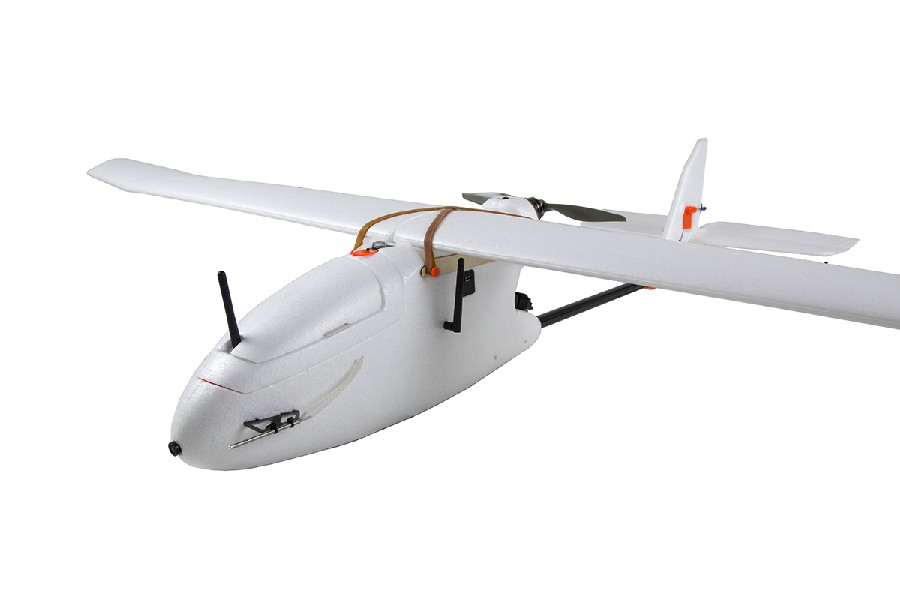
\includegraphics[width=6.5cm,trim=0 0 0 0,clip] {PaperFigures/fixedwing}}
		\subfigure []{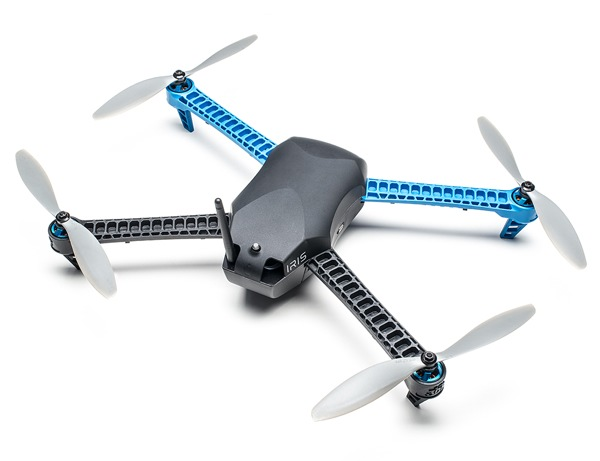
\includegraphics[width=6.5cm,trim=0 0 0 0,clip] {PaperFigures/iris-1}}
		\hspace*{0mm}
	\end{subfigmatrix}
	\caption{Fixed wing (a) and multirotor (b) UAVs}
	\label{fig:fixedMultirotor}
\end{figure}


Weather it is a fixed wing or rotorcraft, UAVs typically accomplish tasks autonomously by following a pre-planned path. Flight paths are typically generated off-line at dedicated ground station and relayed to the UAV over radio. 

\subsection{Ground Stations}
Ground stations are the hardware and software framework used to configure UAV settings, plan missions, and collect mission data. Commercial open source ground stations such as qground control depend on a human operator's knowledge of the environment to plan an obstacle free path. Takeoff, landing, and emergency return-to-home locations are designated in safe clearings capable of accommodating the vehicle. Other tasks such as area surveying and loitering can be assigned at certain points along the mission path. An example of a mission consisting of taking off, surveying, and landing is shown in Figure \ref{fig:groundstationplanning}




\begin{figure}[H]
	\centering
	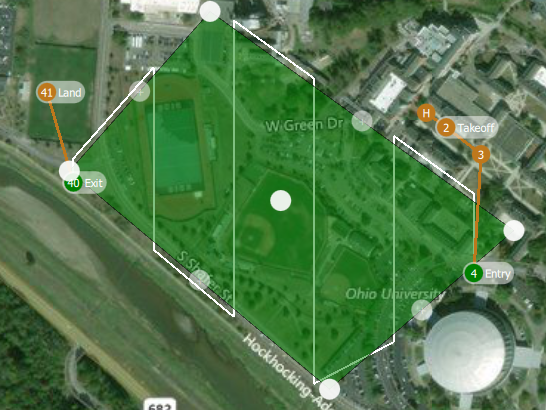
\includegraphics[width=12cm]{PaperFigures/Literature/groundStationPlanning}
	\caption{Ground station software planning a waypoint based mission}
	\label{fig:groundstationplanning}
\end{figure}

These paths are commonly represented as a series of finite waypoints in commercial UAV autopilots such as  the Piccolo \cite{piccolo}, Kestral \cite{kestrel}, and Pixhawk \cite{pix}.


\subsection{Autopilot}
The UAV autopilot is responsible for controlling a pre-planned path and maintaining vehicle stability while under the influence of external wind disturbances. Stable flight while path following is accomplished by implementing feed-back control, navigation, and guidance systems. Feed-back refers to the closure of an open-loop control system which allows a reference error to be calculated between the desired state of the UAV, the reference, and the current state of the UAV. Reference error is used to calculate the necessary actuator output required to modify the vehicles attitude and position while preventing unbounded oscillation. Attitude and position feed-back is provided by the navigation system by sampling on-board sensors such as global position system (GPS) and inertial measurement units (IMUs). Filtering and fusing noisy data from multiple sources is often accomplished through estimation techniques such as the Kalman filter. The guidance system directs the UAV with a commanded heading towards a desired goal, such as a waypoint or path. A high level overview of the autopilots systems can be seen in Figure \ref{fig:autopilotloops}.\\



%\begin{figure}
%	\centering
%	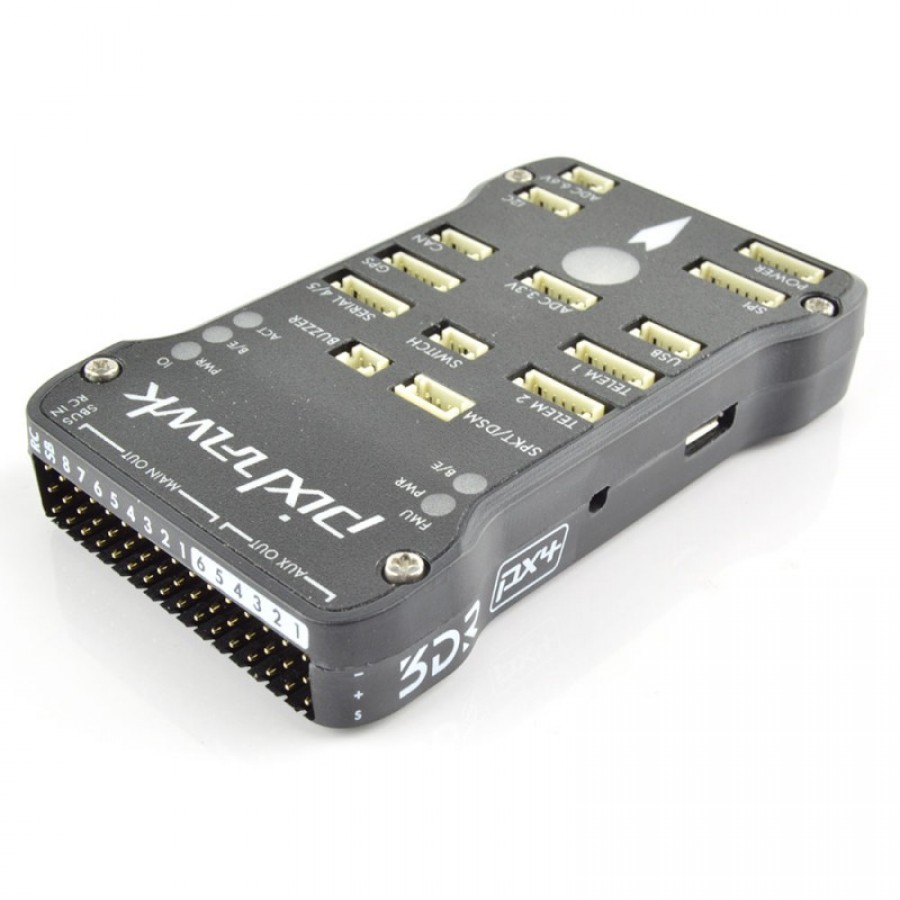
\includegraphics[width=8cm]{PaperFigures/pixhawk}
%	\caption{Pixhawk autopilot}
%	\label{fig:pixhawk}
%\end{figure}
%
%
%



%\begin{figure}
%	\centering
%	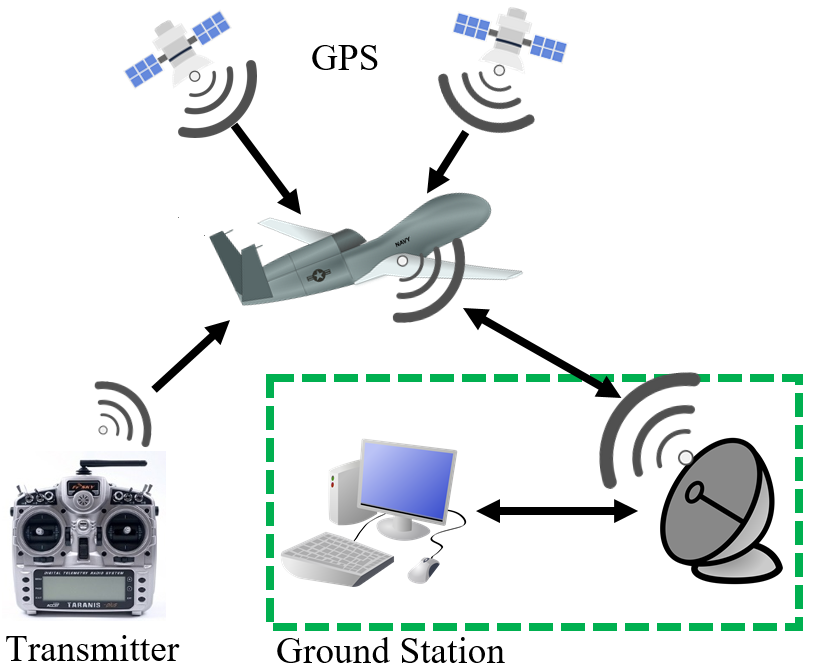
\includegraphics[width=12cm]{PaperFigures/UAS}
%	\caption{Unmanned Aerial System (UAS)}
%	\label{fig:uas}
%\end{figure}

\begin{figure}
	\centering
	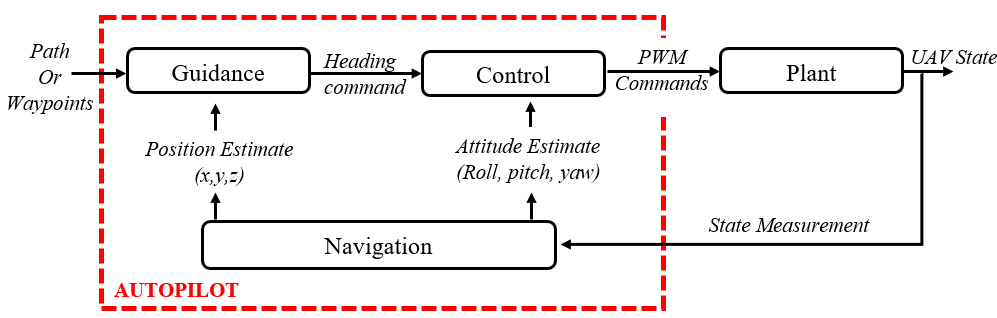
\includegraphics[width=15cm]{PaperFigures/autopilotLoops2}
	\caption{Autopilot's Navigation, Guidance, and Control Architecture}
	\label{fig:autopilotloops}
\end{figure}

\section{Dubins Vehicle Model}
The dynamics of UAVs are often simplified when simulating guidance systems by modeling the UAV as a Dubin's vehicle \cite{frew_cooperative_2007,griffiths_vector_2006,nelson_cooperative_2005,nelson_vector_2006,nelson_vector_2007}. It is assumed that the autopilot's control system is capable of maintaining stability, speed $u$, and can turn the vehicle at a fixed turn rate $\dot{\theta}$. The position of the UAV $\overrightarrow{X}$ at time $t$ is calculated from the integral of the velocity vector $\overrightarrow{U}$, Equation \ref{eq:uavPosition}. Heading $\theta$ is an input from a guidance system. Here the turnrate of the UAV is restricted to $20$ degrees per second.
\begin{equation}
\label{eq:uavVelocity}
\overrightarrow{U}(t) = u \begin{bmatrix}
cos(\theta(t)) \\
sin(\theta(t))
\end{bmatrix}
\end{equation}


\begin{equation}
\label{eq:uavPosition}
\overrightarrow{X}(t) = \overrightarrow{U}dt + \overrightarrow{X}(t-1)
\end{equation}


\begin{equation}
\label{turnRate}
\dot{\theta} \leq 20 deg/s
\end{equation}


\section{UAV Guidance}
On-board guidance systems attempt to minimize the lateral error to the path by commanding a heading pointing to the path. Guidance methods for following a pre-planned path include geometric methods such as carrot chasing \cite{manjunath_application_2016} and control techniques such as proportional-integral-derivative (PID), non-linear guidance laws, and linear quadratic regulator (LQR) \cite{sujit_unmanned_2014}. Due to traditional guidance method's dependence on a path planner to construct an obstacle free and flyable path, these methods often lack a mechanism to avoid new obstacles. Re-planning and relaying a new obstacle free path may be impossible under certain conditions, such as flying beyond line-of-sight. It would be beneficial to include obstacle avoidance into a UAVs guidance system to remove the need to communicate with the ground station or use an on-board path planner which may be accomplished with potential field or vector field. \\


%\subsection{Waypoint Guidance}
%Waypoint guidance aligns the vehicle with the current active waypoint that lies along a pre-planned path. Paths are typically generated off-line and can be optimized for shortest distance traveled and further refined to be flyable for a particular vehicle. Paths may also be optimized to produce flight patterns that increase sensor coverage of an area of interest \cite{wilhelm_direct_2017}. 
%
%If an obstacle lies along that sensor path, the UAV must avoid the obstacle but also return back to the sensor path such that a minimal length of the path is missed during data collection. The number of waypoints that divert around an obstacle effects how closely the UAV tracks the outside of the obstacle and how much of the original path can be traveled. Few obstacle diversion waypoints leads to excess path deviation. Increasing the number of diversion waypoints reduces path deviation, however has diminishing returns. A cost function $\gamma$ can be used to measure the deviation from a planned path while avoiding obstacles with diversion waypoints, shown in Equation \ref{eq:diversionCost}.
%
%\begin{equation}
%\label{eq:diversionCost}
%\begin{aligned}
%\gamma =  \frac{1}{r_O}\int_{0}^{tf}ydt
%\end{aligned}
%\end{equation}
%
%
%An example of a UAV following diversion waypoints is shown in Figure \ref{fig:numWaypointsPath} and the cost associated with increasing number of waypoints in Figure \ref{fig:numWaypoints}.
%
%
%\begin{figure}[H]
%	\begin{subfigmatrix}{2}% number of columns
%		\centering	
%		\subfigure []{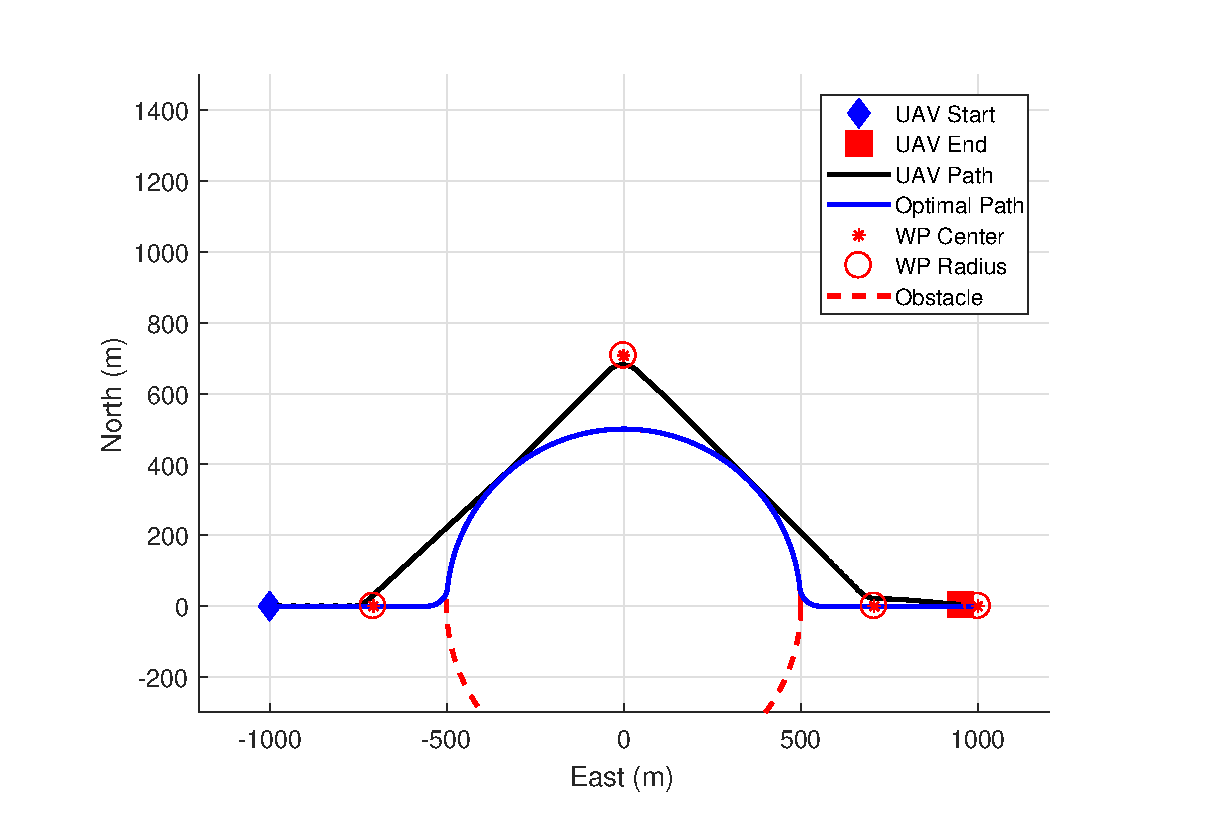
\includegraphics[width=7cm,trim=40 0 60 0,clip] {Figures/Waypoints/1Wpts}}
%		\subfigure []{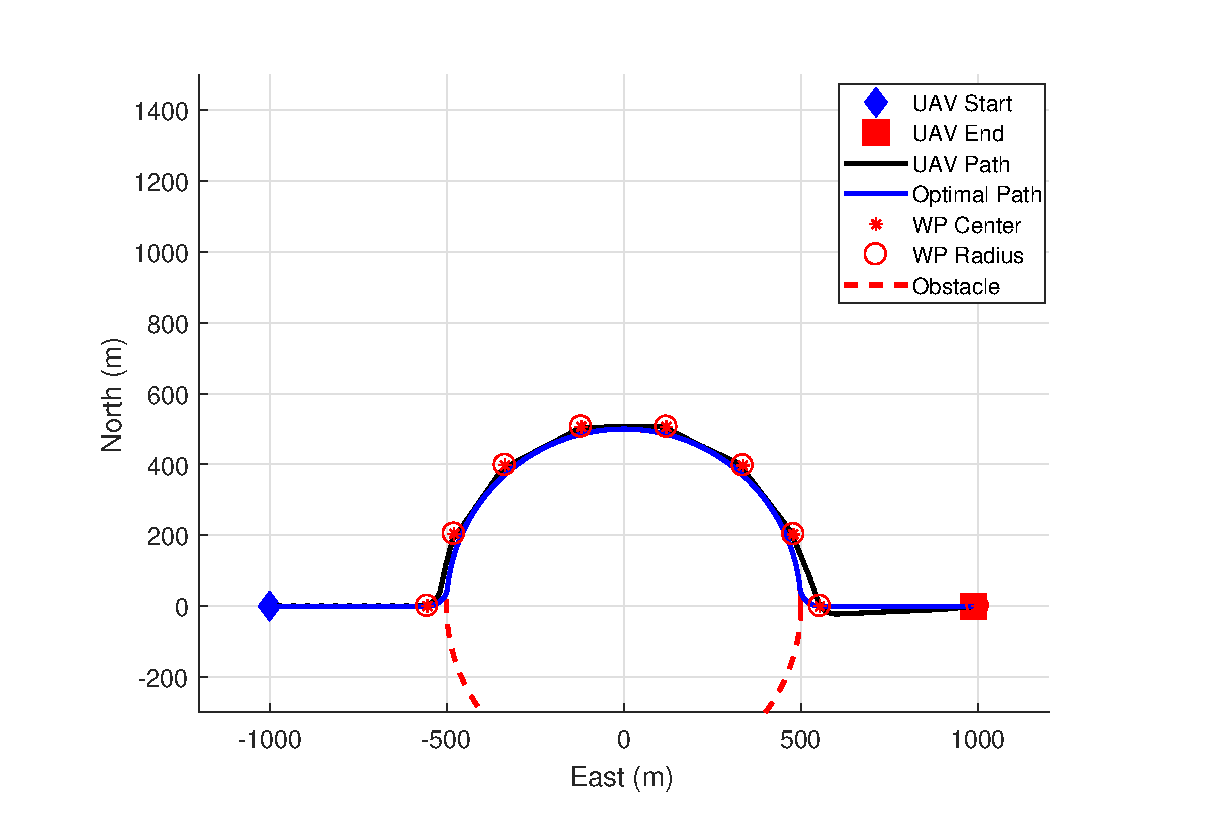
\includegraphics[width=7cm,trim=40 0 60 0,clip] {Figures/Waypoints/6Wpts}}
%		\hspace*{0mm}
%	\end{subfigmatrix}
%	\caption{Obstacle Diversion Waypoints}
%	\label{fig:numWaypointsPath}
%\end{figure}
%
%
%
%\begin{figure}[H]
%	\centering
%	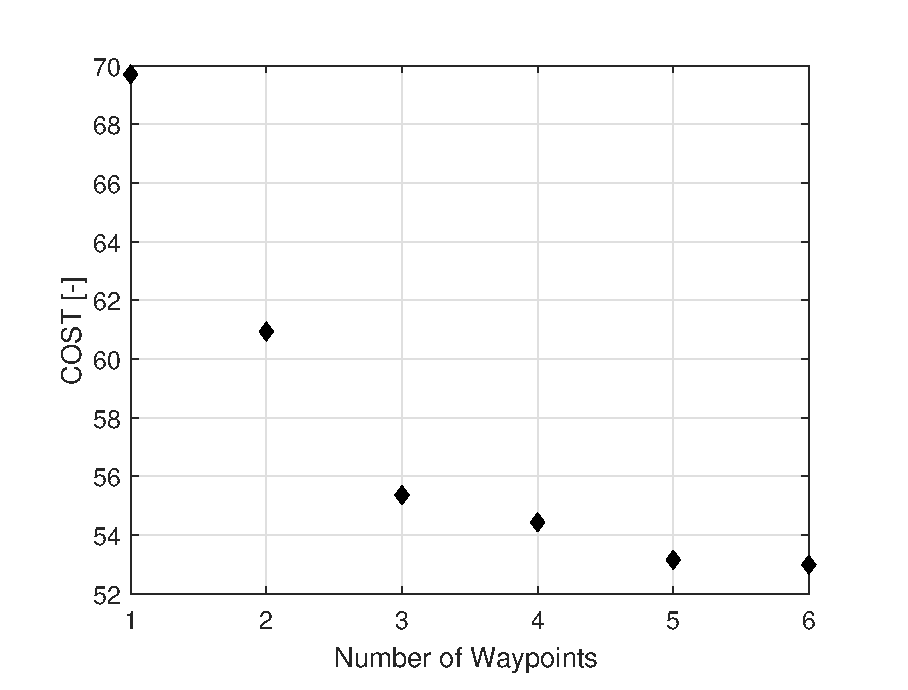
\includegraphics[width=10cm]{Figures/Waypoints/costVnumWpts}
%	\caption{Cost impact versus number of waypoints}
%	\label{fig:numWaypoints}
%\end{figure}




\subsection{Potential Field}

Potential field is based on the principle of driving a point masses state from a high potential to a globally low potential using artificial attractive and repulsive forces \cite{khatib_real-time_1986}. Attractive forces represent a goal, such as a waypoint, that directs the point mass in the goal's direction. Obstacles can be represented as repulsive forces that act locally to push the point mass away. An example of a point mass directed by potential field from a high potential to a globally minimum potential while avoiding an obstacle is shown in Figure \ref{fig:pfobstacle}. Potential field is also capable of acting as a path and trajectory planning algorithm \cite{rimon_exact_1992}, possibly eliminating the off-board path planner. 

\begin{figure}[H]
	\centering
	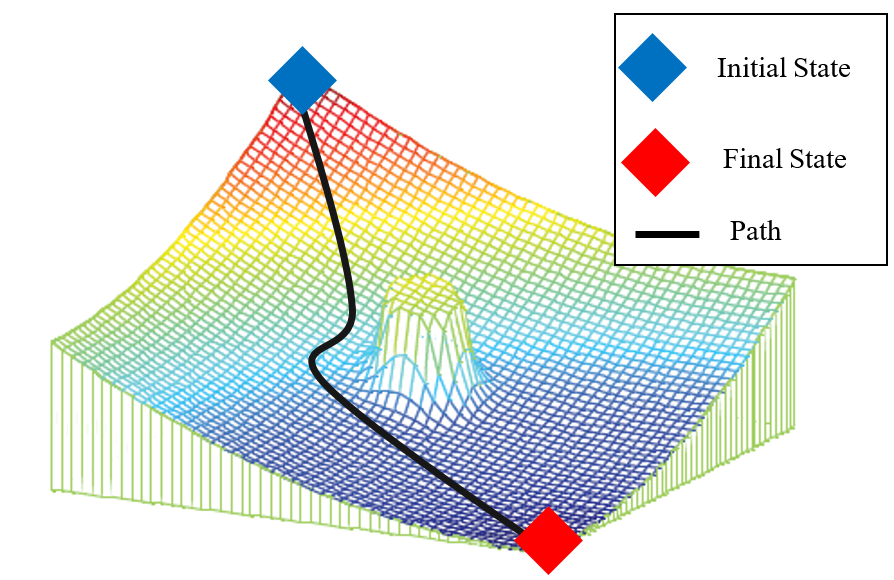
\includegraphics[width=10cm]{PaperFigures/pfObstacle}
	\caption{Single Obstacle Potential Field Gradient \cite{liu_virtual-waypoint_2016}}
	\label{fig:pfobstacle}
\end{figure}


An implementation of potential field on a mobile ground robot equipped with ultrasonic sensors for real-time obstacle detection can be found in \cite{borenstein_real-time_1990,borenstein_vector_1991,koren_potential_1991}. The differential drive robot was guided to a goal with the guidance $\overrightarrow{R}$ while avoiding obstacles. The robot was attracted towards a goal with constant magnitude force $\overrightarrow{F_t}$ located at $(x_t,y_t)$ and a distance $d_t$ from the robot. In the immediate area of the robot, an active window exists which records integer certainty values inside discrete cells. Cells containing an obstacle provide a repulsive force $\overrightarrow{F_{i,j}}$ opposite in direction to the line-of-sight from vehicle to cell location $(x_i,y_j)$, where $(i,j$) represents the cell index, $F_{cr}$ is a constant repulsive force, $W$ the vehicle's width, $C_{i,j}$ a cell's certainty, and $d_{i,j}$ the distance to the center of the cell with respect to robots center.

\begin{equation}\label{eq:vffHeading}
\overrightarrow{R} = \overrightarrow{F_r} + \overrightarrow{F_t}
\end{equation} 



\begin{figure}[H]
	\centering
	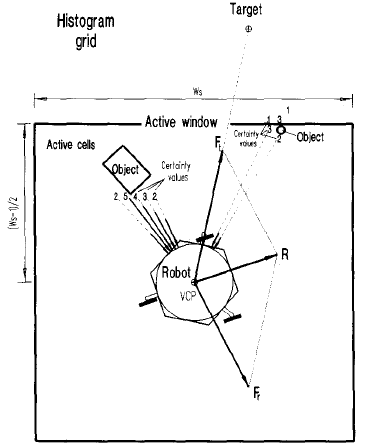
\includegraphics[width=7cm]{PaperFigures/histogram}
	\caption{Virtual force field histogram acting on a mobile robot \cite{borenstein_vector_1991}}
	\label{fig:histogram}
\end{figure}

\begin{equation}\label{eq:vffRepulse}
\overrightarrow{F_{i,j}} = \frac{F_{cr}W^nC_{i,j}}{d^n_{i,j}} \bigg( \frac{x_i-x_0}{d_{i,j}}\hat{x} + \frac{y_i-y_0}{d_{i,j}}\hat{y}\bigg)
\end{equation}

\noindent
The total repulsive force exerted on the robot is determined by summing the active cells, shown in Equation \ref{eq:vffRepulseSum}


\begin{equation}\label{eq:vffRepulseSum}
\overrightarrow{F_r} = \sum_{i,j}\overrightarrow{F_{i,j}}
\end{equation}


\begin{equation}\label{eq:vffGoal}
\overrightarrow{F_t} = F_{ct} \bigg( \frac{x_t-x_0}{d_{t}}\hat{x} + \frac{y_t-y_0}{d_{t}}\hat{y}\bigg)
\end{equation}

\noindent
Summing together attractive and repulsive forces produce a vector $\overrightarrow{R}$ that can be used for heading guidance, shown in Equation \ref{eq:vffHeading}.

\begin{equation}\label{eq:vffHeading}
\overrightarrow{R} = \overrightarrow{F_r} + \overrightarrow{F_t}
\end{equation}

Major drawbacks to potential field were identified in \cite{koren_potential_1991} consisting of local minimum and oscillations in corridors. Local minimum are solutions in the potential field that are caused by the close spacing of obstacles which may result in a well that can trap the system into a local stable point prior to reaching the global minimum. A scenario similar to that shown in Figure \ref{fig:pfobstacle} with more obstacles results in a trap situation where the state settles into a well on the gradient, shown in Figure \ref{fig:pfLocalMin}. Additionally, closely spaced obstacles may also be difficult to pass between, shown in Figure \ref{fig:vff}a. Oscillations can also be experienced near obstacles or in narrow passages at high speeds, shown in Figure \ref{fig:vff}b.



 

\begin{figure}[H]
	\begin{subfigmatrix}{2}% number of columns
		\centering
		\subfigure []{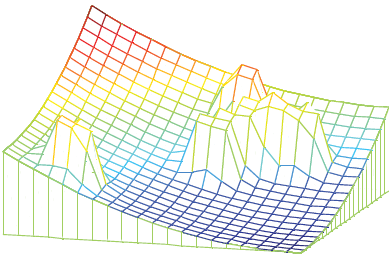
\includegraphics[width=7cm] {PaperFigures/pfObstacleLocalMin}}
		\subfigure []{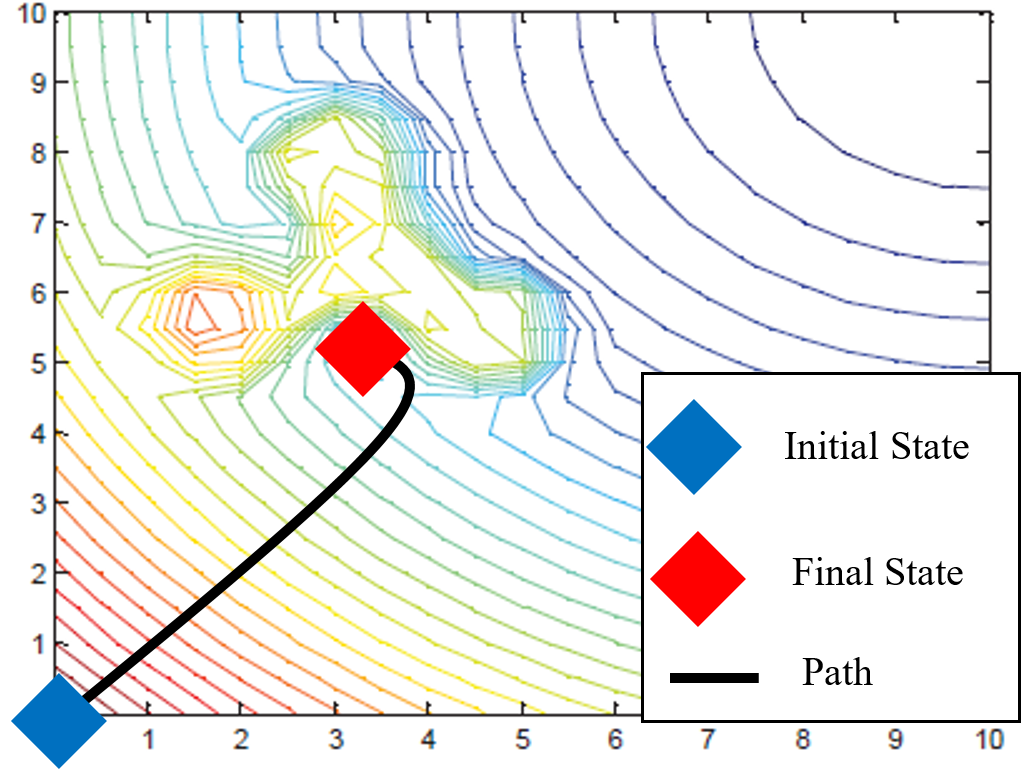
\includegraphics[width=7cm] {PaperFigures/pfObstacleLocalMinTopology}}
	\end{subfigmatrix}
	\caption{Potential Field Local Minimum \cite{liu_virtual-waypoint_2016}}
	\label{fig:pfLocalMin}
\end{figure}

Proposed solutions to local minimum include object clustering and virtual waypoint method \cite{liu_virtual-waypoint_2016}, virtual escaping route \cite{kim_escaping_2009}, and use of navigation functions \cite{goerzen_survey_2010}. Oscillations in potential field were addressed in \cite{lei_tang_novel_2010} and \cite{li_efficient_2012}.

\begin{figure}[H]
	\begin{subfigmatrix}{2}% number of columns
		\centering
		\subfigure []{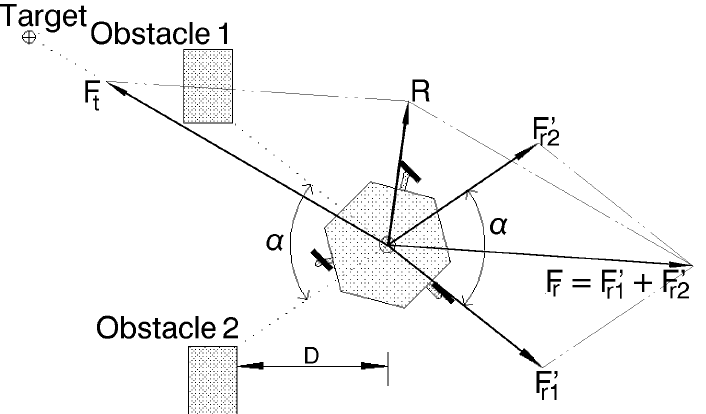
\includegraphics[width=9cm] {PaperFigures/multipleObsVff}}
		\subfigure []{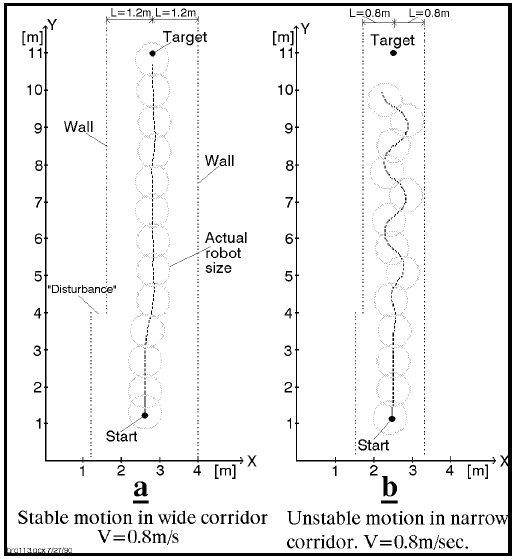
\includegraphics[width=6cm] {PaperFigures/unstableCooridorMotionVff}}
	\end{subfigmatrix}
	\caption{Potential Field Local Minimum \cite{liu_virtual-waypoint_2016}}
	\label{fig:vff}
\end{figure}

Navigation functions \cite{goerzen_survey_2010} and obstacle clustering \cite{liu_virtual-waypoint_2016} have been used to prevent local minimums in potential field. Navigation functions relate kinematic constraints to the gradient potential to produce a bounded and local minimum free solution \cite{rimon_exact_1992}. Clustering closely spaced obstacles into a single and equally repulsive obstacle prevents local minimum from forming, shown in Figure \ref{fig:obstacleclustering}.  

\begin{figure}[H]
	\centering
	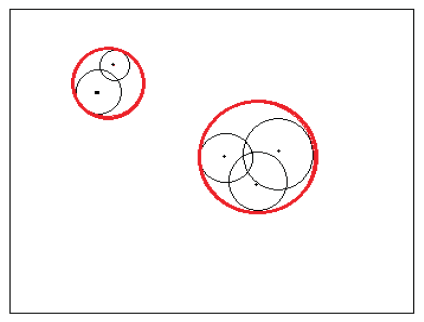
\includegraphics[width=6cm]{PaperFigures/obstacleClustering}
	\caption{Obstacle Clustering \cite{liu_virtual-waypoint_2016}}
	\label{fig:obstacleclustering}
\end{figure}

Potential Field's ability to avoid obstacles and combine path planning, trajectory planning, and control into a single computationally inexpensive system makes it an attractive motion control system for robots seeking a singular point, even with the limitations discussed in \cite{koren_potential_1991}. Unlike the mobile ground robots in \cite{borenstein_real-time_1990}, fixed wing UAVs must maintain a minimum forward velocity, have limited turning radius, and cannot converge to a single point. Vehicles with velocity and turn rate constraints may not return to a pre-planned path once the obstacle has been avoided, shown in Figure \ref{fig:vffSimulated}. Methods that direct a UAV to a path instead of a discrete point has been achieved with Lyapunov and gradient vector fields. 


\begin{figure}[H]
	\centering
	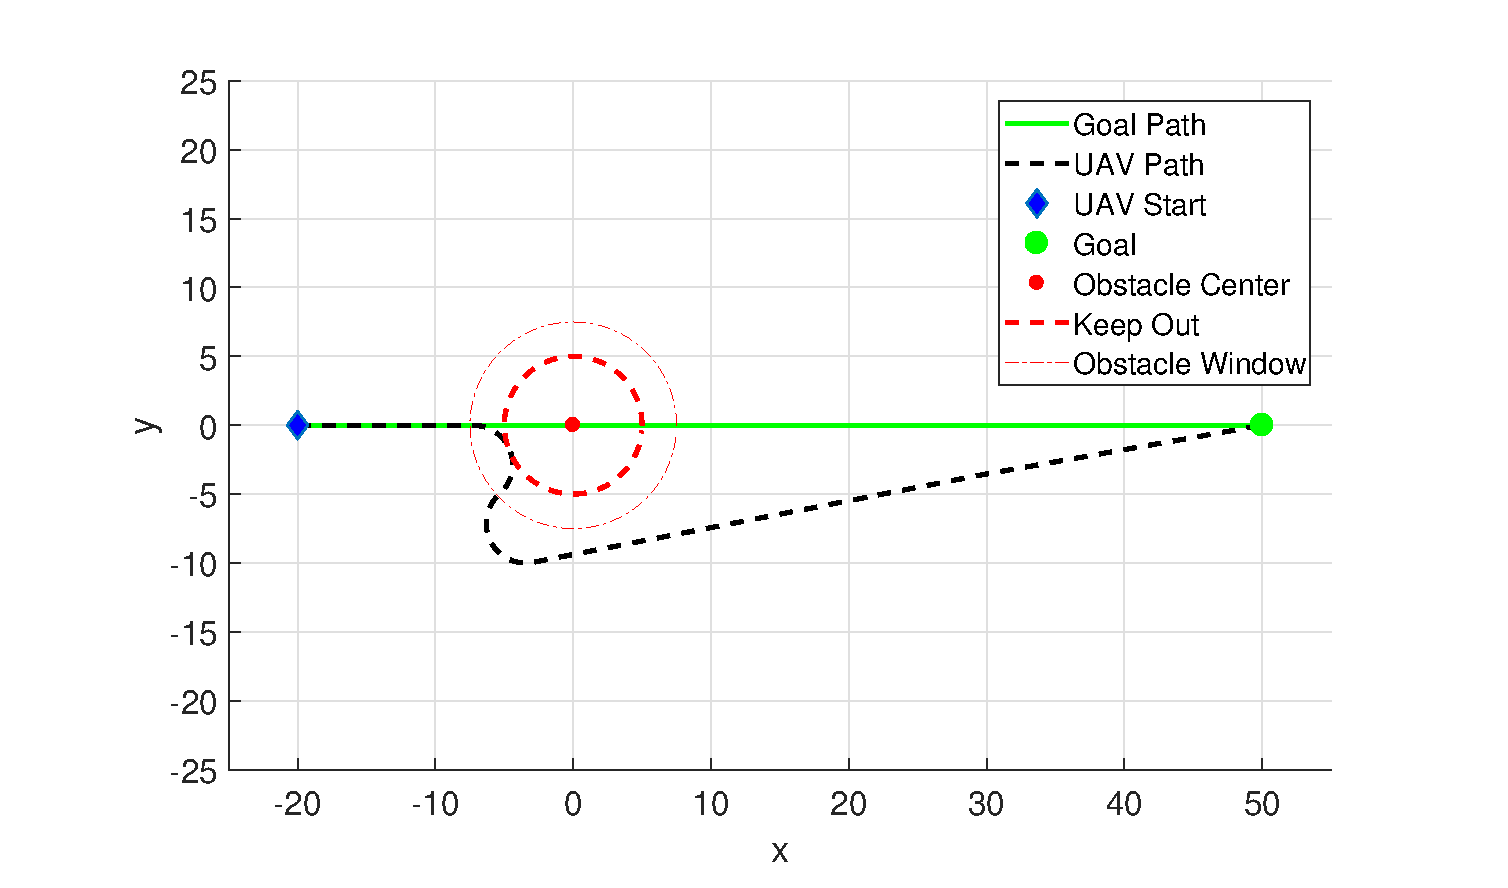
\includegraphics[width=15cm]{PaperFigures/Literature/vffSimulated}
	\caption{UAV avoiding obstacle with VFF Guidance}
	\label{fig:vffSimulated}
\end{figure}


%\subsection{\hl{Path Following Vector Field Guidance}}
%
%Path following can be accomplished with vector fields which produce a heading guidance that asymptotically converges and circulates a path. A comparison between vector field and waypoint guidance techniques was presented in \cite{sujit_unmanned_2014} where each method was evaluated based on its complexity, robustness, and accuracy. Vector field produced guidance that was both robust to external wind disturbances while maintaining a low cross track error.
%
%
%The UAV guidance system is responsible for taking high level pre-planned paths from the ground station and providing a reference heading command to the control system. Several methods for path following guidance were investigated in \cite{sujit_unmanned_2014} consisting of carrot chasing \cite{manjunath_application_2016}, non-linear guidance law, pure line-of-sight \cite{fortuna_cascaded_2015}, linear quadratic regulator \cite{capello_simulation-based_2012}, and vector field method \cite{nelson_cooperative_2005}. A Monte Carlo simulation with wind disturbances was conducted for the guidance methods above in \cite{sujit_unmanned_2014} to determine each method's performance based on accuracy, robustness, and control effort. The vector field method followed the path with the least tracking error and control effort which is the primary goal of path following. 


%\section{Vector Field Guidance}
%\subsection{Introduction to Vector Field Guidance}
% \hl{Vector Field is a guidance and control approach that can be used to transition a robotic system from an initial state to a final state. Final states, or goals, act as artificial attractive forces that pull on the robotic system while obstacles act as artificial repulsive forces that push the robotic system away. Classes of vector fields can be categorized as point seeking or path following algorithms. Potential Field and Virtual Force Field (VFF) methods converge to a single point and avoid obstacles by applying artificial attractive and repulsive forces. Lyapunov and Gradient Vector Fields provide guidance that asymptotically converges and follows a path. Obstacle avoidance has been achieved with Gradient Vector Fields by assigning repulsive weights to a convergence term. Weights currently act as a high level specification of the desired guidance behavior and may be further optimized.} 

\subsection{Lyapunov Vector Fields}



Lyapunov vector fields for converging and following straight and circular paths were described in \cite{nelson_cooperative_2005}. For converging and following a straight path, a guidance vector $\chi^{d}$ is determined in Equation \ref{eq:lyapunovStraight}, where $\chi^{\infty}$ is the course approach angle, $y$ is the lateral distance to the path, and $k$ is a positive constant that determines the rate of transition between convergence and following. An example of a Lyapunov vector field converging and following a straight line is shown in Figure \ref{fig:vfPathPrimitives}a.



% and are defined in Equations \ref{eq:lyapunovStraight} and \ref{eq:lyapunovCirc} respectively.

%------ Nelson VF equations -----
\begin{equation}\label{eq:lyapunovStraight}
\chi^d(y) = -\chi^{\infty}\frac{2}{\pi}\tan^{-1}(ky)
\end{equation}



For converging and following a circular path, a guidance vector $\chi^{d}$ is determined in Equation \ref{eq:lyapunovCirc}, where $\gamma$ is the UAVs angular position with respect to the circle, $r$ is the paths radius, $d$ is the distance from the circles center, and $k$ is a positive constant that determines the transition behavior. An example of a Lyapunov vector field for converging and following a circular path is shown in Figure \ref{fig:vfPathPrimitives}b.

\begin{equation}\label{eq:lyapunovCirc}
\chi^d(d) = \gamma-\frac{\pi}{2}-\tan^{-1} \bigg(k \frac{d-r}{r} \bigg)
\end{equation}


\begin{figure}
	\centering
	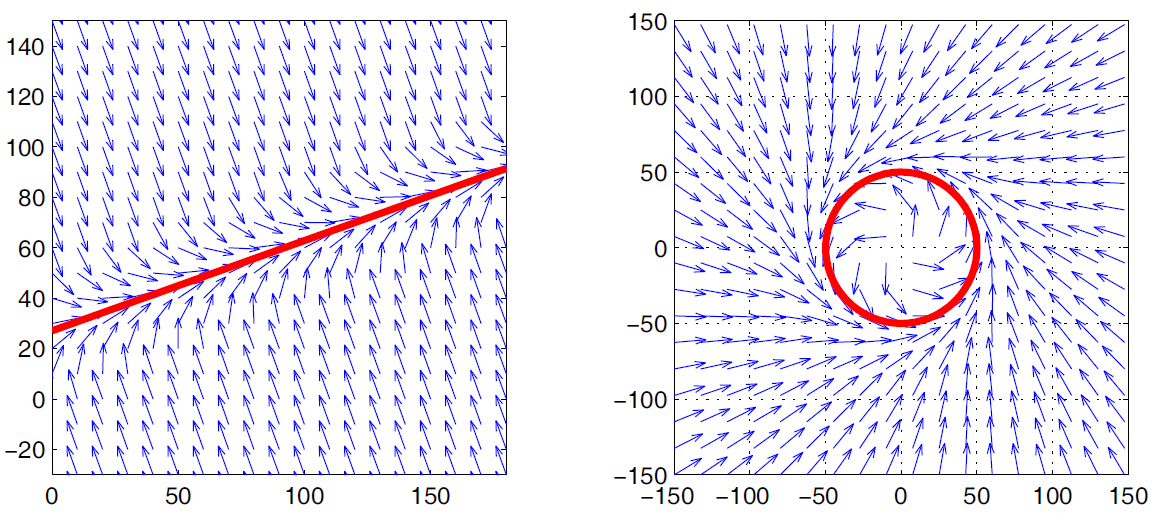
\includegraphics[width=13cm]{PaperFigures/nelsonLyapunov}
	\caption{Lyapunov vector field for straight line and circular primitives \cite{nelson_cooperative_2005}}
	\label{fig:vfPathPrimitives}
\end{figure}




%A circular Lyapunov vector field can be generated by the methodology described in \cite{frew_cooperative_2007}. Given the Lyapunov function:
%
%
%$y$ lateral distance from path \\
%$\chi$ difference between direction of path and course of UAV \\
%$k$ positive constant that influences the rate of transition \\
%$\chi^{\infty}$  course approach angle at large distance \\
%$\chi^{d}$ is commanded heading \\
%
%$d$ radial distance UAV from center of orbit \\
%$\gamma$ angular position with respect to orbit center \\
%$r$ orbit radius \\
%
%
%
%
%\begin{figure}[H]
%	\begin{subfigmatrix}{2}% number of columns
%		\centering	
%		\subfigure []{\includegraphics[width=7.5cm] {Figures/lineConvcirc}}
%		\subfigure []{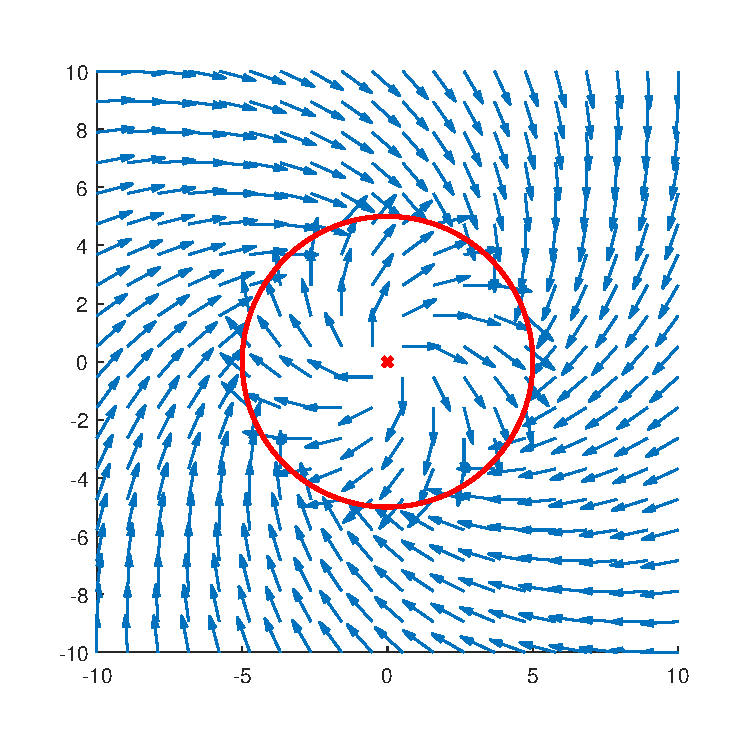
\includegraphics[width=7.5cm] {Figures/circConvCirc}}
%		\hspace*{0mm}
%	\end{subfigmatrix}
%	\caption{Vector field converging and following a) straight path b) circular path}
%	\label{fig:vfPrimitives}
%\end{figure}
%
%
%\begin{equation}\label{eq:lyapunovfunction}
%V(x,y) = (r^2 - r_d^2)^2
%\end{equation}
%where $r$ is given by the equation
%\begin{equation}
%r = \sqrt{x^2+y^2}
%\end{equation}
%and the total time derivative of Equation \ref{eq:lyapunovfunction} is
%\begin{equation}\label{eq:totaltimederivative}
%\dot{V}(x,y) = \nabla{V} \cdotp [\dot{x},\dot{y}]^{T}
%\end{equation}
%Utilizing the following equation to select the desired relative velocity $\dot{x}$ and $\dot{y}$
%\begin{equation}
%\overrightarrow{V}_{Lyapunov}\!=\!\begin{bmatrix} \dot{x_d} \\ \dot{y_d} \end{bmatrix}\!= \alpha\!\left(\dfrac{-v}{r}\right)\!\begin{bmatrix} x \dfrac{r^2-r_d^2}{r^2+r_d^2} + y \dfrac{2 r r_d}{r^2+r_d^2} \\[12pt] y \dfrac{r^2-r_d^2}{r^2+r_d^2} - x \dfrac{2 r r_d}{r^2+r_d^2} \end{bmatrix}
%\end{equation}
%and assuming $\alpha$\,=\,1 and $r$\,=\,1, the final Lyapunov VF equation is generated:
%\begin{equation}\label{eq:lyapunovvf}
%\overrightarrow{V}_{Lyapunov} = \frac{v}{r^2+r_d^2} \begin{bmatrix} - x (r^2-r_d^2) - y (2 r r_d) \\[6pt] - y (r^2-r_d^2) + x (2 r r_d) \end{bmatrix}
%\end{equation}



%Straight and circular path vector fields can be selectively activated throughout flight to form more complex paths, shown in \cite{nelson_cooperative_2005,nelson_vector_2006,nelson_vector_2007,jung_unmanned_2016}. Lyapunov vector field for curved path following was presented in \cite{griffiths_vector_2006} which may allow for more complex paths and eliminates the need to switch between vector fields. \\


%
%==========================\\
%Lyapunov vector fields produce heading guidance that asymptotically converges and circulates along a path passing through waypoints. Paths can be built from straight line and circular arc primitives taking UAV kinematic constraints into consideration. Vector Fields that guide to straight line and circular paths was introduced in \cite{nelson_cooperative_2005}. Farther away from the path, vectors are constant and point in the direction perpendicular to the path. Within a transition region the vectors begin to rotate and point more parallel to the path. Vectors on the path point directly in the direction of the path. Lyapunov vector fields for straight line and circular arcs are shown in Figure \ref{fig:nelsonlyapunov}.
%
%=====================================

Straight and circular path vector fields can be selectively activated throughout flight to form more complex paths, shown in \cite{nelson_cooperative_2005,nelson_vector_2006,nelson_vector_2007,jung_unmanned_2016} and Figure \ref{fig:urbanfollowingnelson}. Each path primitive has a vector field associated with it and determining which field to use can be approached in two different ways. Fields from all of the primitives can be summed together similar to the attractive and repulsive forces in potential field. Second, fields can be selectively activated and deactivated based on the position of the UAV. Summing together vector fields, as pointed out in \cite{nelson_cooperative_2005}, can result in several problems including dead zones, sinks, and singularities. Selectively activating each vector field as a UAV nears waypoints was used in \cite{nelson_cooperative_2005,nelson_vector_2006,nelson_vector_2007,jung_unmanned_2016}.

\begin{figure}[H]
	\centering
	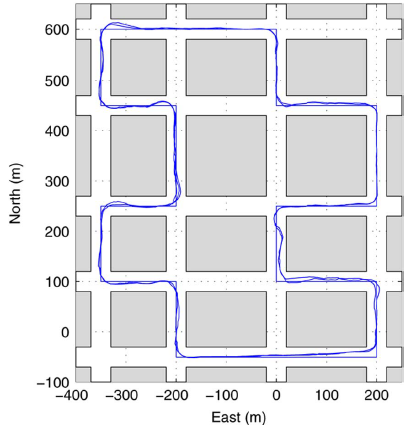
\includegraphics[width=7cm]{PaperFigures/urbanFollowingNelson}
	\caption{Straight path following in urban environment \cite{nelson_cooperative_2005} using Lyapunov Vector Field}
	\label{fig:urbanfollowingnelson}
\end{figure}

Lyapunov Vector field construction for curved paths was presented in \cite{griffiths_vector_2006} and is shown in Figure \ref{fig:griffiths}. Constructing a Vector Field for an arbitrary curve may allow for more complex paths and could eliminate the need for switching between primitives. 

\begin{figure}[H]
	\centering
	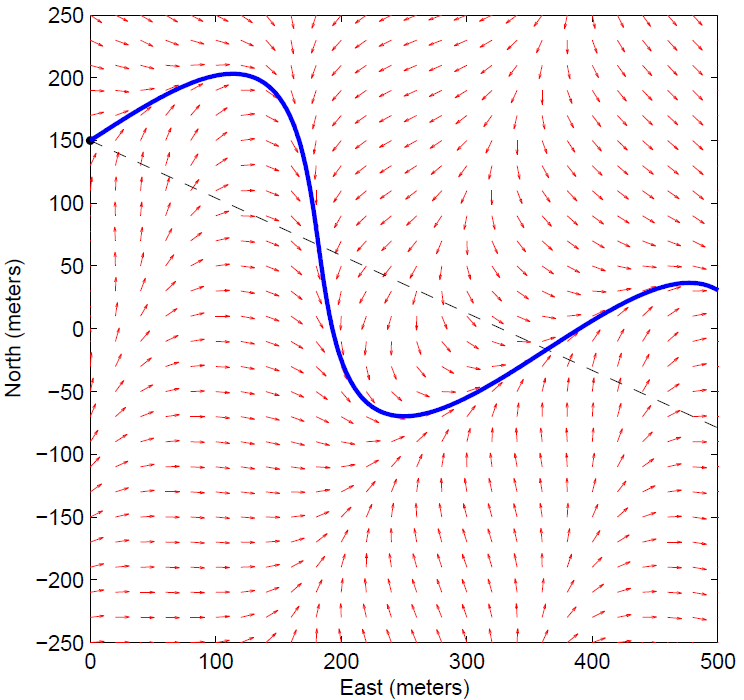
\includegraphics[width=7cm]{PaperFigures/griffiths}
	\caption{Lyapunov vector field approach curved path asymptotically \cite{griffiths_vector_2006}}
	\label{fig:griffiths}
\end{figure}


Primitive circular vector fields were modified in \cite{frew_lyapunov_nodate,frew_cooperative_2007} via non-linear coordinate transformations to produce elliptical \ref{fig:lyapunovFrew}a, or racetrack \ref{fig:lyapunovFrew}b, fields. Transforming the circular field as a function of a Kalman filter's covariance matrix when sensing an uncertain target was investigated in \cite{frew_cooperative_2007}. 

\begin{figure}[h]
	\begin{subfigmatrix}{2}% number of columns
		\centering
		\subfigure []{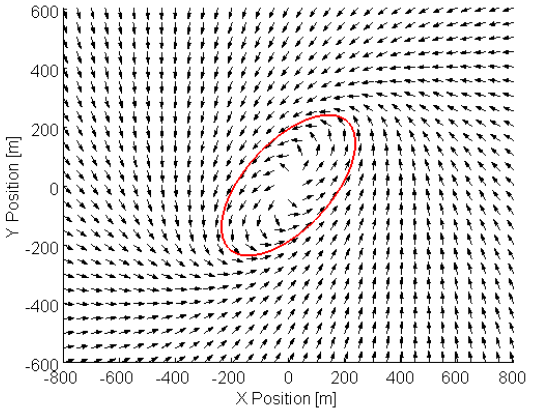
\includegraphics[width=8cm] {PaperFigures/lyapunovFrewUncertain}}
		\subfigure []{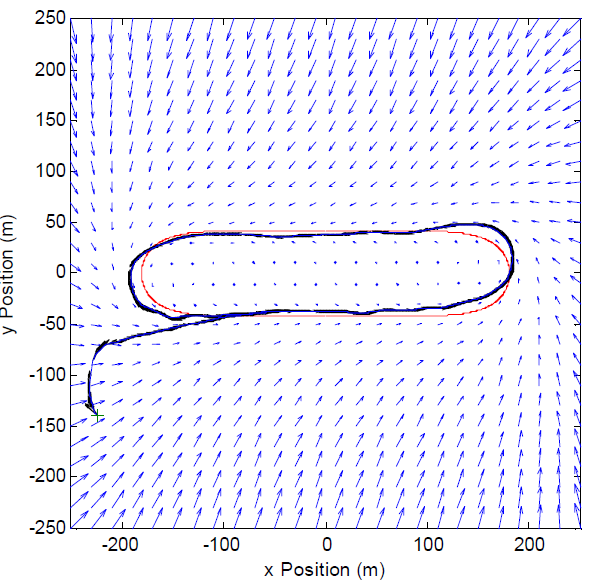
\includegraphics[width=6.25cm] {PaperFigures/lyapunovFrew}}
		%		\hspace*{1cm}
	\end{subfigmatrix}
	\caption{Elliptical VF produced by non-linear coordinate transformations a)\cite{frew_cooperative_2007} and b) \cite{frew_lyapunov_nodate}}
	\label{fig:lyapunovFrew}
\end{figure}

Target tracking Tangent Plus Lyapunov Vector Field (TPLVF) was introduced in \cite{chen_tracking_2009} that produced shorter paths compared to Lyapunov alone. Outside of the standoff circle, tangent vectors provided the shortest distance to a standoff circle. Inside the standoff circle, no tangent lines exist and Lyapunov was used in its place. Figure \ref{fig:lyapunovChen} shows the difference in paths taken for Lyapunov and tangent vector fields outside the standoff circle. The TPLVF was later used for path planning to avoid obstacles in \cite{chen_uav_2013} while \cite{liang_tangent_2017} constructed a tangent vector field for curved paths.

\begin{figure}
	\centering
	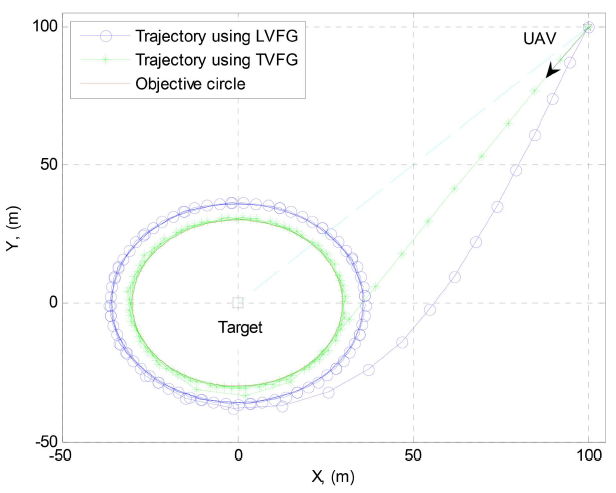
\includegraphics[width=10cm]{PaperFigures/lyapunovChen}
	\caption{Tangent plus lyapunov vector fields for shortest path target tracking \cite{chen_uav_2013}}
	\label{fig:lyapunovChen}
\end{figure}


\subsection{Path Planning Vector Fields}
Another use of vector fields is a high level specification for heuristic path planning algorithms \cite{pereira_framework_2016}. An optimal Rapid Random Trees (RRT*) algorithm used a vector field as a guide to explore the configuration space of the UAV for an obstacle free path. Branches extend from the root, or initial location of the UAV, randomly throughout the map with a finite deviation from the initial vector field. When a branch encounters an obstacle it is trimmed and no longer explored. The path of minimum cost, or least distance, is selected for the UAV to use as a reference path. An example of the algorithm is shown in Figure \ref{fig:rrtvf}.

\begin{figure}[H]
	\centering
	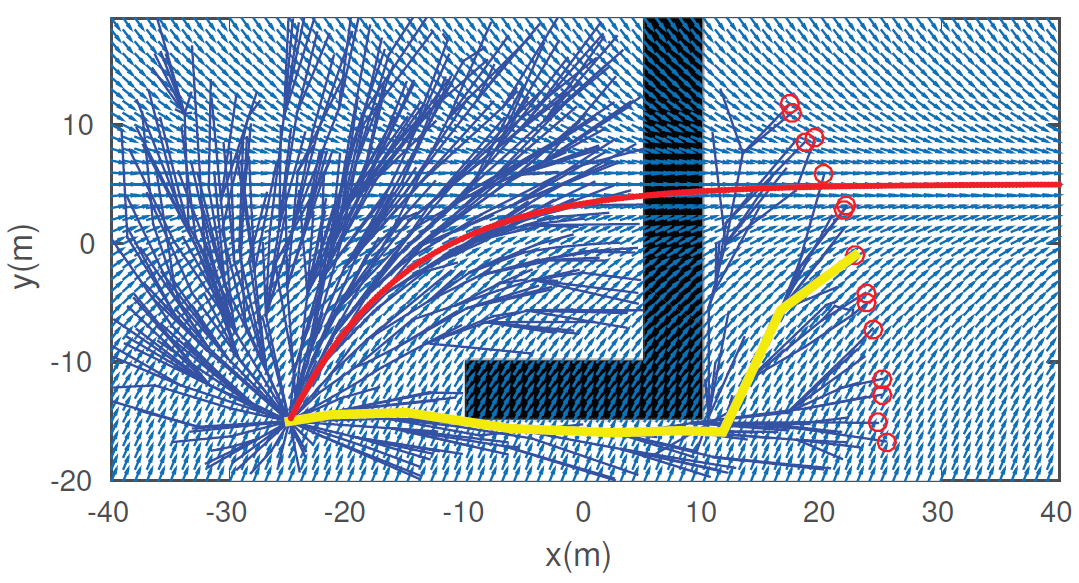
\includegraphics[width=12cm]{PaperFigures/rrtVF}
	\caption{RRT* path planner with a VF used as a task specification \cite{pereira_framework_2016}}
	\label{fig:rrtvf}
\end{figure}


A VF was constructed inside a configuration space with edges defined by Delauny triangulation (DT) in \cite{pimenta_fully_2007}.  A simulation of a robot traversing a vector field inside a set of DTs can be seen in Figure \ref{fig:cdtVF}. Vector fields designed to stay inside a region of DTs may be used with optimal path planning algorithms for navigating urban environments \cite{md_simplex_2017}.


\begin{figure}
	\centering
	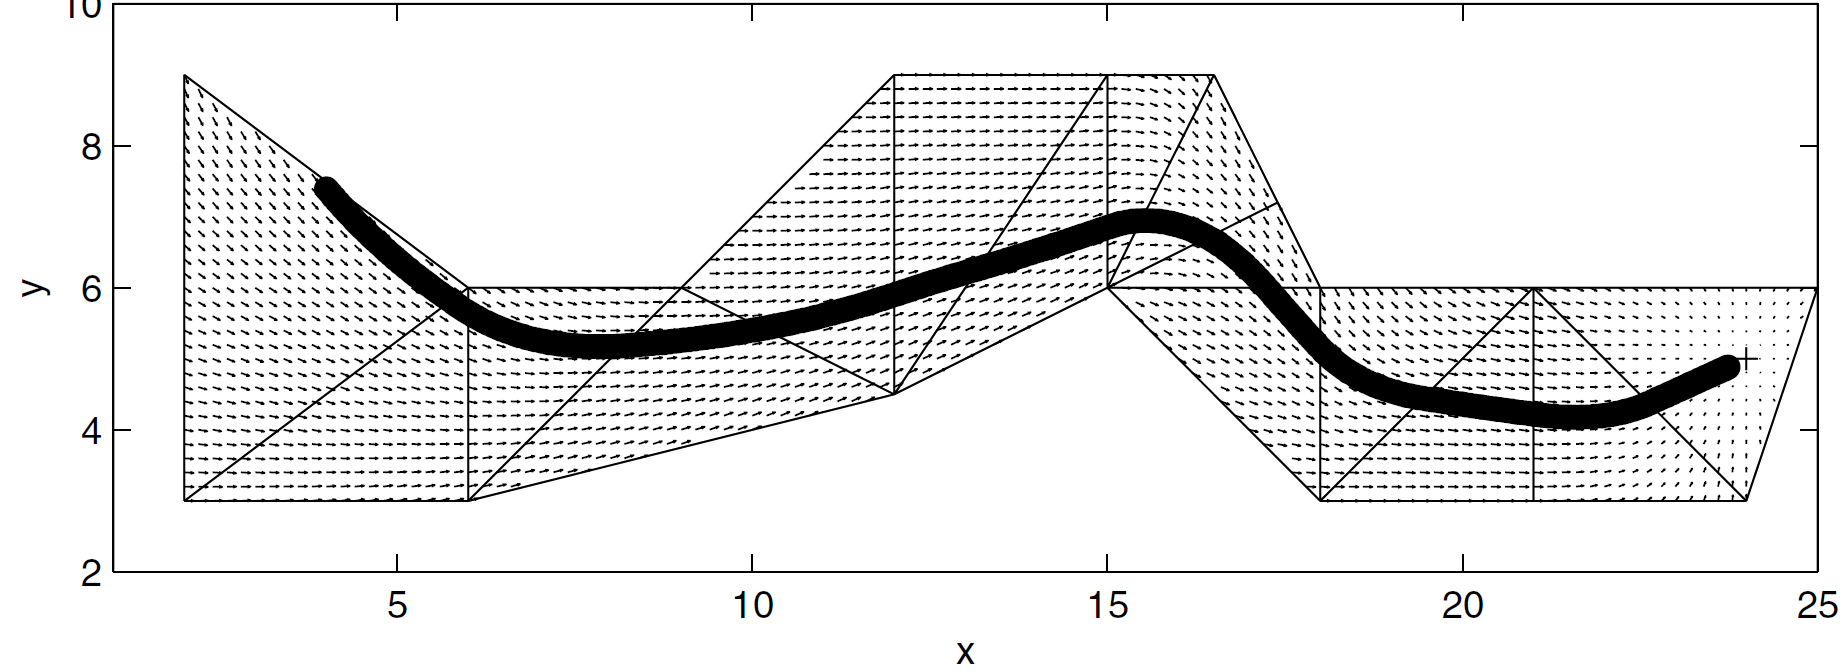
\includegraphics[width=15cm]{PaperFigures/cdtVF}
	\caption{Vector field within a set of delaunay triangles \cite{pimenta_fully_2007}}
	\label{fig:cdtVF}
\end{figure}

So far all of the vector field methods discussed have avoided obstacles by planning paths around them. Paths are typically calculated at the ground station and if communication is lost a new path may not be relayed to a UAV encountering a new obstacle. A possible solution is using vector fields to provide a repulsive force such as that seen in \cite{panagou_motion_2014,zhou_vector_2014} [wwc]. 

\subsection{Gradient Vector Field}
The Gradient Vector Field (GVF) method produces a similar field, however has several advantages over LVFs. GVF produces an \textit{n}-dimensional vector field that converges and circulates to both static and time varying paths \cite{goncalves_artificial_2009}. Additionally, convergence, circulation, and time-varying terms that make up the GVF are decoupled from each other allowing for easy weighting of the total field \cite{goncalves_circulation_2010}. GVFs converge and circulate at the intersection, or level set, of $n-1$ dimensional implicit surfaces ($\alpha_i:\mathbb{R}^n\rightarrow\mathbb{R} | i=1,...,n-1$). The integral lines of the field are guaranteed to converge and circulate the level set when two conditions are met: $1)$ the implicit surface functions are positive definite and $2)$ have bounded derivatives. Consider the space with dimensions in set \textbf{q}:

%The Goncalves Vector Field (GVF) method for producing vector fields has several advantages over the Lyapunov vector field generation methods.


\begin{equation}
\mathbf{q} = \begin{bmatrix} x_1, x_2, ..., x_{n}\end{bmatrix}
\end{equation}

\noindent
The total vector field $\overrightarrow{V}$ is calculated by:
\begin{equation}\label{eq:GVF}
\overrightarrow{V} = G \nabla V + H \wedge_{i=1}^{n-1}\nabla_q\alpha_i  - LM(\alpha)^{-1} a(\alpha)
\end{equation}

\noindent
or in component form:

\begin{equation}\label{simpleGVF}
\overrightarrow{V} = \overrightarrow{V}_{conv} + \overrightarrow{V}_{circ} + \overrightarrow{V}_{tv} 
\end{equation}	

\noindent
where $\overrightarrow{V}_{conv}$ produces vectors that converge to the path, $\overrightarrow{V}_{circ}$ produces vectors that circulate the path, and $\overrightarrow{V}_{tv}$ is a feed-forward term that produces vectors accounting for a time varying path. The scalars $G$,$H$, and $L$ weight convergence, circulation, and time varying components respectively. 

\noindent
Convergence is calculated by:

\begin{equation}
% Total field with Conv, Circ, and Time
\overrightarrow{V}_{conv} = G \nabla V  
\label{convOnly}
\end{equation}

\noindent
where scalar $G$ is multiplied by the gradient of the definite potential function $V$:

\begin{equation}
\label{potentialV}
V = -\sqrt{{\alpha_1}^2 + {\alpha_2}^2}
\end{equation}


\noindent
Circulation is calculated by taking the wedge product of the gradient:

\begin{equation}
% Total field with Conv, Circ, and Time
\overrightarrow{V}_{circ} =  \wedge_{i=1}^{n-1}\nabla_q\alpha_i 
\label{circOnly}
\end{equation}

\noindent
In the case of $(n=3)$ the wedge product simplifies as the cross product:

\begin{equation}
% Total field with Conv, Circ, and Time
\overrightarrow{V}_{circ} =  \nabla_q\alpha_1 \times \nabla_q\alpha_2 
\label{circOnlySimp}
\end{equation}

\noindent
The feed-forward time-varying component is calculated by:
\begin{equation}
\label{tv}
\overrightarrow{V}_{tv} = M^{-1}a
\end{equation}

\noindent
where,

\begin{equation}
\label{mMatrix}
M =\begin{bmatrix}
\nabla\alpha_1^T \\
\nabla\alpha_2^T \\
(\nabla\alpha_1 \times \nabla\alpha_2)^T
\end{bmatrix}
\end{equation}

\begin{equation}
\label{aVector}
a =\begin{bmatrix}
\frac{\partial \alpha_1}{\partial t} \quad   \frac{\partial \alpha_2}{\partial t} \quad   0
\end{bmatrix}^T
\end{equation}


In \cite{goncalves_artificial_2009,goncalves_circulation_2010,goncalves_vector_2010} GVFs were constructed to control the velocity $\dot{q}$ of a holonomic robot by $\dot{q}=h$. Constant speed  $u$ was controlled by calculating the weighting scalars $G$,$H$, and $L$ that maintained the condition $||\dot{q}|| = u$. Other studies normalized the vector $\overrightarrow{V}$ and used it as a heading guidance while assuming velocity is held constant by the autopilot \cite{gerlach_autonomous_2014}[wwc]. Assuming velocity is controlled by a separate system frees up the vector field scalars to modify field behavior for other applications, such as obstacle avoidance. 
 
 
 The standoff tracking and avoidance scenario presented in [wwc] used GVF as a heading guidance and static GVF weights to specify high level guidance behavior. A fixed UAV was tasked with loitering around a slow moving ground target while avoiding obstacles. A circular attractive time-varying vector field $\overrightarrow{V}_{p}$ was attached to a moving ground target and summed with repulsive obstacle vector fields $\overrightarrow{V}_{o}$ centered at the obstacles to provide the guidance $\overrightarrow{V}$ in Equation \ref{summedAttRepulsive}. 
 
 
 \begin{equation}
 \overrightarrow{V} = \overrightarrow{V}_{p}+P\overrightarrow{V}_{o}
 \label{summedAttRepulsive}
 \end{equation}
 
 \noindent
 The strength of repulsive obstacle fields were weighted by the hyperbolic tangent decay function $P(d)$ in Equation \ref{repulsiveDecay}, where $d$ is the range to the obstacle and $R$ is the radius of the decay, shown in Figure \ref{fig:tanhLit}
 
 \begin{equation}
 P = -R\frac{tanh(2\pi d-\pi)-2}{2}
 \label{repulsiveDecay}
 \end{equation}

\begin{figure}[H]
	\centering
	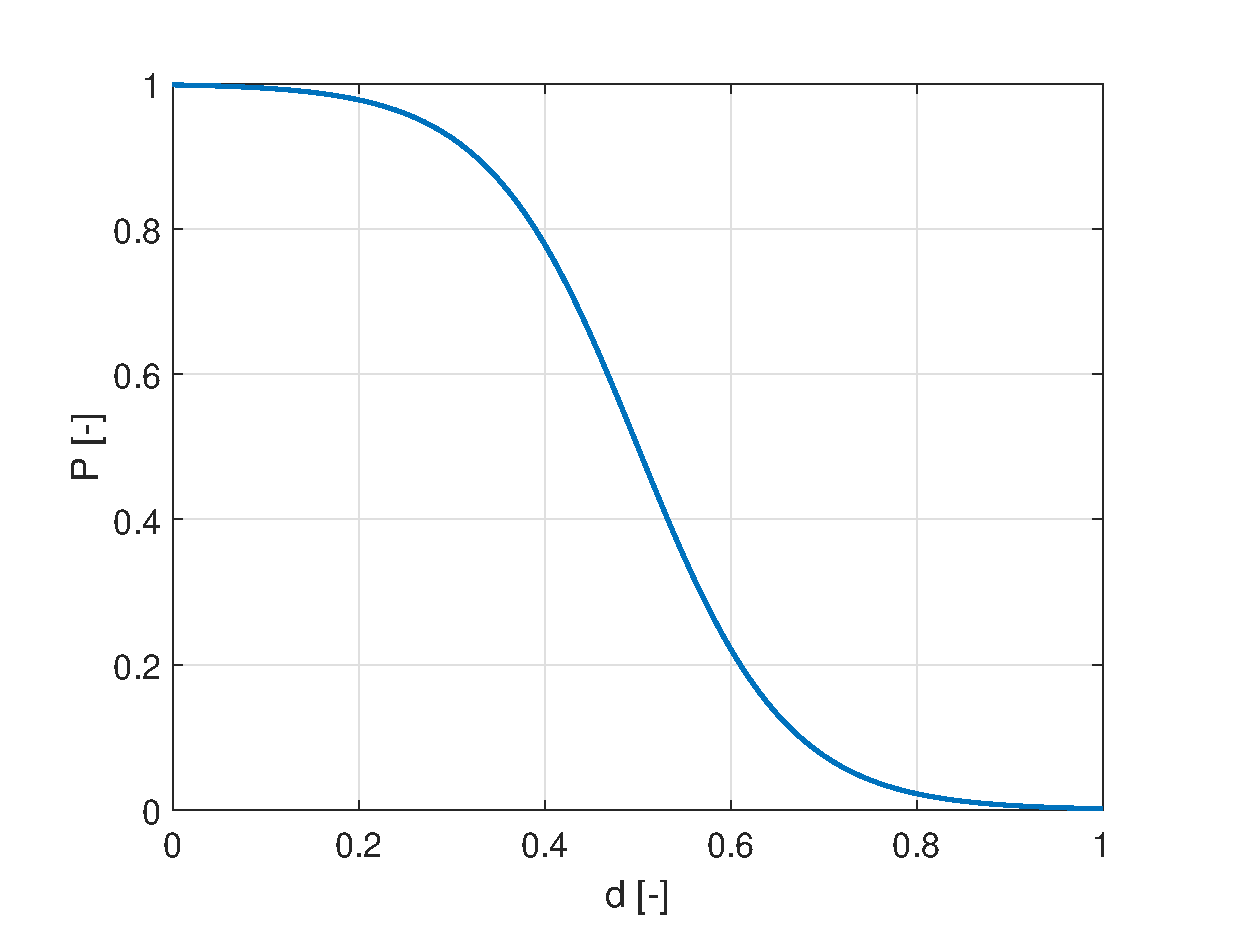
\includegraphics[width=12cm]{PaperFigures/Literature/tanh}
	\caption{}
	\label{fig:tanhLit}
\end{figure}

 
 \noindent
 The performance of LVF [21] and GVF \cite{goncalves_artificial_2009,goncalves_circulation_2010,goncalves_vector_2010} were compared for their cross track error with respect to the loiter circle in [wwc]. GVF was shown to have less cross track error compared to LVF due to the compensation for a time-varying vector field attached to the moving target. The path of the fixed wing UAV tracking a slow moving ground target while avoiding static obstacles is shown in Figure \ref{fig:gvfMovingTarget}


\begin{figure}[H]
	\centering
	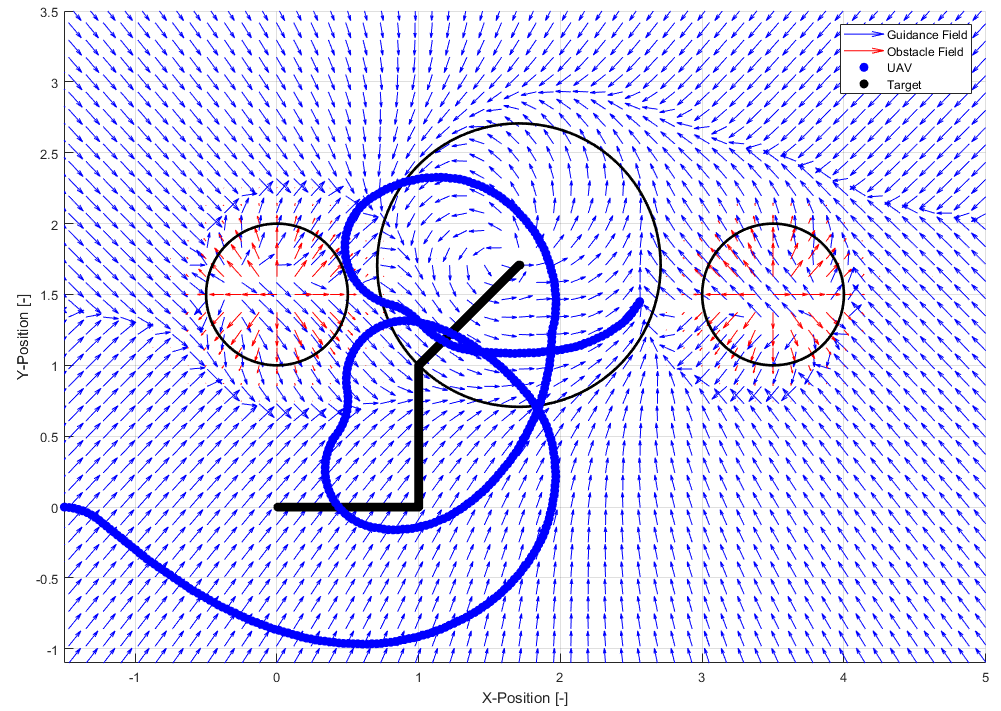
\includegraphics[width=10cm]{PaperFigures/gvfMovingTarget}
	\caption{Place holder image of UAV following ground target \cite{wwc}}
	\label{fig:gvfMovingTarget}
\end{figure}

Summing attractive and repulsive vector fields may result in null guidance where the fields cancel, providing no guidance. The presence of singularities were mentioned briefly in \cite{nelson_cooperative_2005} and observed in \cite{panagou_motion_2014}. For fixed wing UAVs the lack of guidance may prevent the UAV from avoiding an obstacle, while multi-rotor UAVs may end up in a trap situation. Singularities may be present at any location where a goal field and obstacle field are of equal strength. Detecting singularities and modifying the GVF for an improved obstacle avoidance is the contribution of this research.



%The GVF weights are decoupled from each term calculation, therefore modifications to the GVF weights do not require a new derivation of the resulting field. Magnitude of the weights effectively scales the contribution of each term. Negating the GVF weights has been used to provide a repulsive field for obstacle avoidance in \cite{wwc} for a UAV tracking a moving loiter circle. Assigning weights \textbf{G=-1} and \textbf{H=L=0} rotates the attractive field vectors in Figure \ref{fig:gvfCircAttractive}b 180$^\circ$ about the tail of each vector, which is shown in Figure \ref{fig:gvfRepulsiveRadius}a. Note how the repulsive field vectors point away from the circular curve for the entire configuration space. Encircling an obstacle by a path produces vectors that may provide guidance into the obstacle, which is not desired. Reducing the radius to be smaller than the radius of the obstacle produces a GVF with nearly all vectors directing away. 
%
%
%\begin{figure}[H]
%	\begin{subfigmatrix}{2}% number of columns
%		\centering	
%		\subfigure []{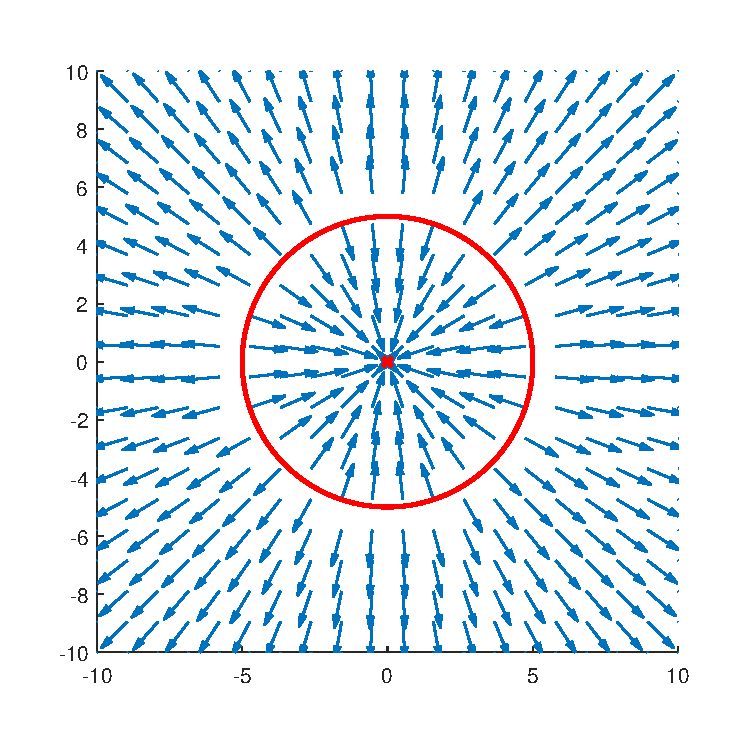
\includegraphics[width=6.5cm] {PaperFigures/compWithoutTitles/circRepulsive}}
%		\subfigure []{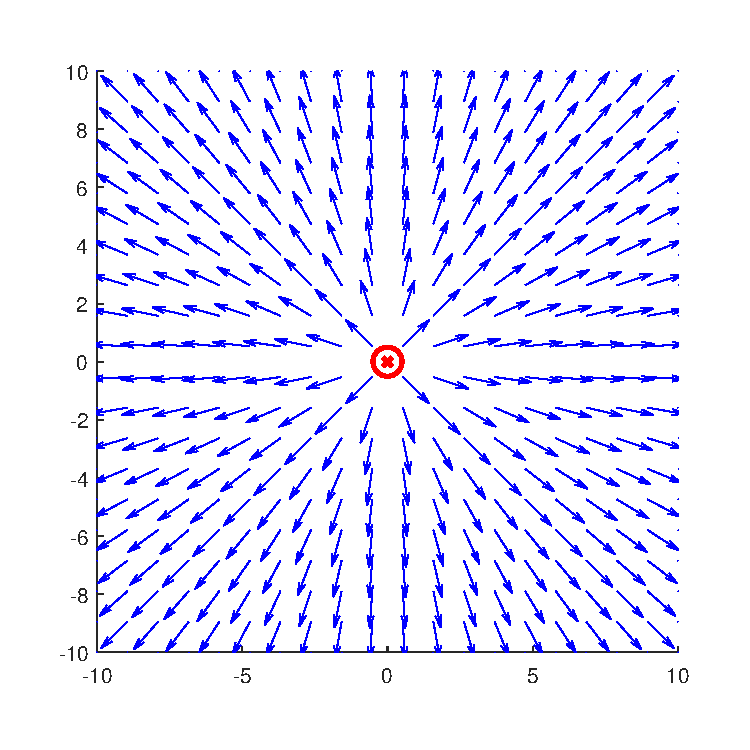
\includegraphics[width=6.5cm] {PaperFigures/compWithoutTitles/circRepulsiveSmallr}}
%		\hspace*{0mm}
%	\end{subfigmatrix}
%	\caption{Repulsive field with large path radius (a) and small radius (b)}
%	\label{fig:gvfRepulsiveRadius}
%\end{figure}
%
%The strength of the repulsive field was varied as a function of proximity $d$ by multiplying the repulsive field by a decay function $P$ bounded on the interval [-1,0], shown in Equation \ref{repulsiveDecay} and Figure \ref{fig:tanhICUAS2018}. The radius $R$ is the distance from the center of the field where vectors have effectively zero strength. 
%
%\begin{equation}
%P = R\frac{tanh(2\pi d-\pi)+1}{2}
%\label{repulsiveDecay}
%\end{equation}
%
%\begin{equation}
%\vec{v}_{repulsive} = -G||\vec{v_{conv}}||P
%\label{replulsiveField}
%\end{equation}
%
%
%
%\begin{figure}[H]
%	\begin{subfigmatrix}{2}% number of columns
%		\centering	
%		\subfigure []{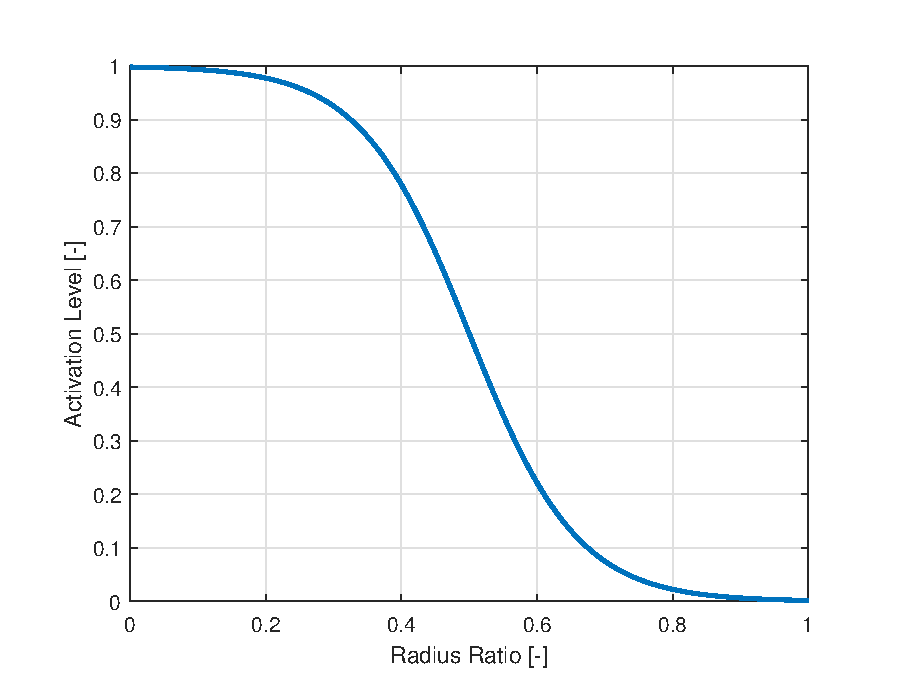
\includegraphics[width=8cm] {PaperFigures/tanh_ICUAS2018}}
%		\subfigure []{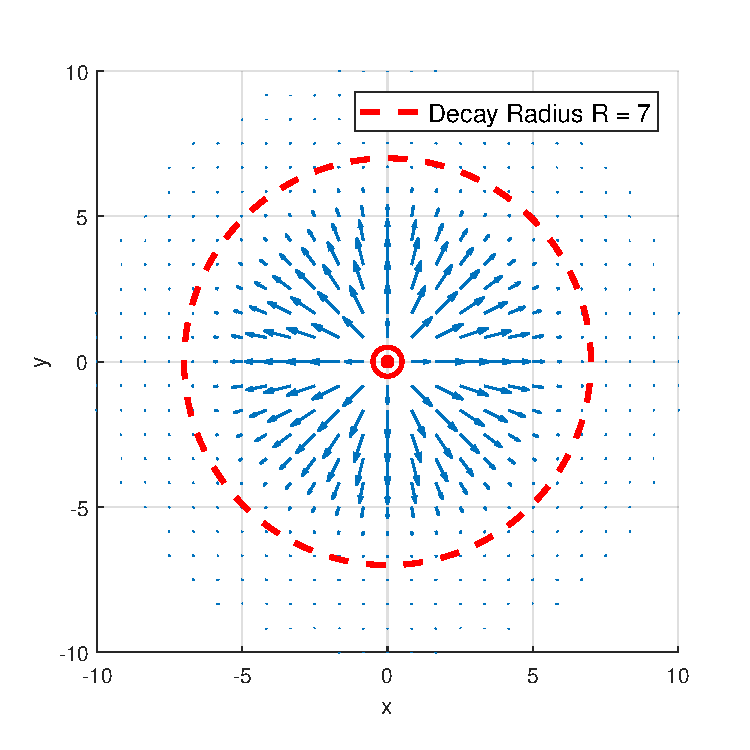
\includegraphics[width=7cm] {PaperFigures/repulsiveFields/circRepulsiveDecay}}
%		\hspace*{0mm}
%	\end{subfigmatrix}
%	\caption{Repulsive field activation \cite{wwc} (a) resulting repulsive field (b)}
%	\label{fig:tanhICUAS2018}
%\end{figure}
%
%
%Attractive and repulsive fields were added together similar to that in \cite{panagou_motion_2014} and the resulting vector shown in Equation \ref{summedAttRepulsive}. The resultant heading vector was used to guide a UAV to track a moving loiter circle while avoiding static obstacles, shown in Figure \ref{fig:gvfMovingTarget}.
%
%\begin{equation}
%\vec{V} = \vec{v}_{attractive}+\vec{v}_{repulsive}
%\label{summedAttRepulsive}
%\end{equation}
%
%
%
%\begin{figure}[h]
%	\centering
%	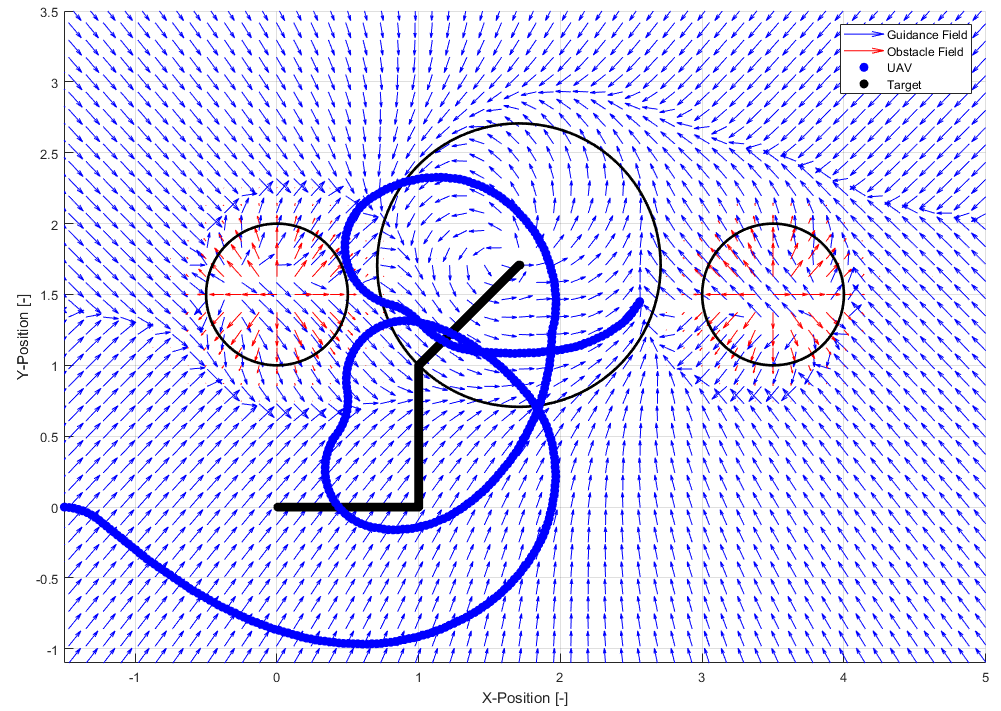
\includegraphics[width=10cm]{PaperFigures/gvfMovingTarget}
%	\caption{Place holder image of UAV following ground target \cite{wwc}}
%	\label{fig:gvfMovingTarget}
%\end{figure}
%
%
%GVF weights have been used for high level specification of the desired behavior for a UAV, whether it be for convergence, circulation, or avoidance. Repulsive GVFs have considered obstacle fields that strictly repel. The strictly repulsive guidance is effective at directing a UAV away from an obstacle, but provides no information on how to circumnavigate one. Additionally, further specification on the minimum radius and strength of the repulsive field may be useful in preventing a UAV from violating the obstacle circle. A preliminary simulation shows that a UAV encountering an obstacle while tracking a path may result in violation of the obstacle space, shown in Figure \ref{fig:singleobstacle}. UAVs traveling at lower velocities
%may also enter a trap situation where the guidance is confined to an infinite loop.
%\pagebreak
%
%\begin{figure}[h]
%	\centering
%	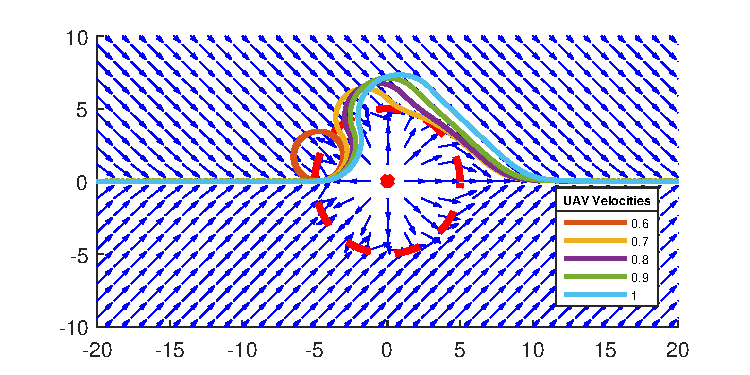
\includegraphics[width=12cm]{PaperFigures/singleObstacle}
%	\caption{Strictly repulsive obstacle on straight path}
%	\label{fig:singleobstacle}
%\end{figure}
%
%
%Adding circulation \textit{\textbf{H=1}} to the GVF in Figure \ref{fig:singleobstacle} prevented the trap situation for a velocity $u = 0.6$ and reduced the circumnavigation distance, which is shown in Figure \ref{fig:singleobstacleWithCirc}. Specifying vector field weights as functions of a UAV's state may enable an optimal guidance for obstacle avoidance. 
%
%\begin{figure}[h]
%	\centering
%	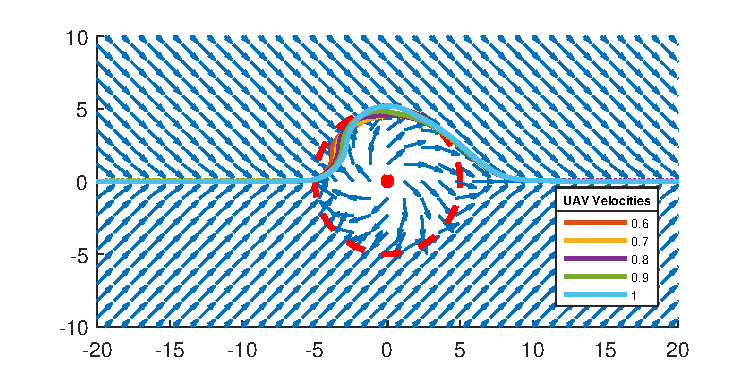
\includegraphics[width=12cm]{PaperFigures/singleObstacleWithCirc}
%	\caption{Circulating repulsive obstacle on straight path}
%	\label{fig:singleobstacleWithCirc}
%\end{figure}




\section{Literature Review Summary}
UAVs are versatile tools that can be used for remote data collection without putting a pilot in harms way. Tasks are typically accomplished by following a series of waypoints that lie along an obstacle free and flyable pre-planned path. When unplanned or previously unknown obstacles are discovered along the UAVs planned path, a new obstacle free and flyable path may have to be generated which could be impossible if the ground station is not reachable. Methods such as potential field and vector field have been used to avoid obstacles without re-planning mission waypoints. Potential field is not ideal for fixed wing UAVs since it converges to a singular point whereas Lyapunov and gradient vector fields converge and follow paths. Summing paths and negating field weights can be used for obstacle avoidance, however have so far been used only as high level specification of guidance behavior. Gradient vector field allows for easy weighting of individual convergence and circulation terms therefore is the best candidate for providing an optimized avoidance field.Determining repulsive field weigths and decay radius has not been optimized for obstacle avoidance. Additionally, characterization of vector field singularities in a summed field has yet to be addressed in literature due to most methods avoiding summation entirely. The contribution of this research is to characterize GVF singularities and provide an optimized decay radius and circulation weight for repulsive fields that minimize path deviation. 

\chapter{Methodology}

%\section{Dubins Vehicle}
%The dynamics of UAVs are often simplified when simulating guidance systems by modeling the UAV as a Dubin's vehicle \cite{frew_cooperative_2007,griffiths_vector_2006,nelson_cooperative_2005,nelson_vector_2006,nelson_vector_2007}. It is assumed that the autopilots control system is capable of maintaining stability, speed $u$, and can turn the vehicle at a fixed turn rate $\dot{\theta}$. The position of the UAV $\overrightarrow{X}$ at time $t$ is calculated from the integral of the velocity vector $\overrightarrow{U}$, Equation \ref{eq:uavPosition}. Heading is an input from a guidance system, such as waypoint, potential field, or vector field.
%
%\begin{equation}
%\label{eq:uavVelocity}
%\overrightarrow{U}(t) = u \begin{bmatrix}
%cos(\theta(t)) \\
%sin(\theta(t))
%\end{bmatrix}
%\end{equation}
%
%
%\begin{equation}
%\label{eq:uavPosition}
%\overrightarrow{X}(t) = \overrightarrow{U}dt + \overrightarrow{X}(t-1)
%\end{equation}
%
%
%\begin{equation}
%\label{turnRate}
%\dot{\theta} \leq 20 deg/s
%\end{equation}


%\subsection{MOVE TO METHODOLOGY}
%The GVF weights are decoupled from each term calculation, therefore modifications to the GVF weights do not require a new derivation of the resulting field. Magnitude of the weights effectively scales the contribution of each term. Negating the GVF weights has been used to provide a repulsive field for obstacle avoidance in \cite{wwc} for a UAV tracking a moving loiter circle. Assigning weights \textbf{G=-1} and \textbf{H=L=0} rotates the attractive field vectors in Figure \ref{fig:gvfCircAttractive}b 180$^\circ$ about the tail of each vector, which is shown in Figure \ref{fig:gvfRepulsiveRadius}a. Note how the repulsive field vectors point away from the circular curve for the entire configuration space. Encircling an obstacle by a path produces vectors that may provide guidance into the obstacle, which is not desired. Reducing the radius to be smaller than the radius of the obstacle produces a GVF with nearly all vectors directing away. 
%
%
%\begin{figure}[H]
%	\begin{subfigmatrix}{2}% number of columns
%		\centering	
%		\subfigure []{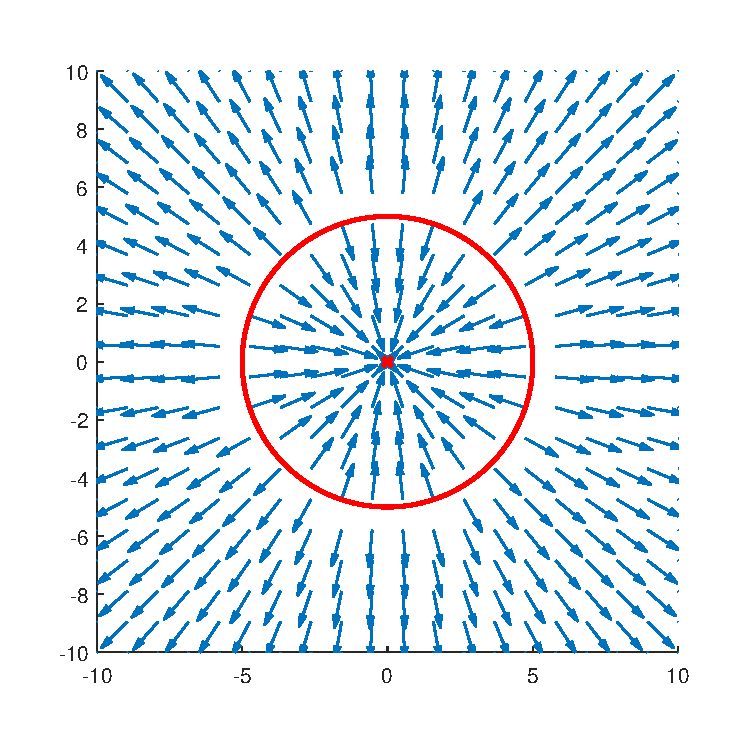
\includegraphics[width=6.5cm] {PaperFigures/compWithoutTitles/circRepulsive}}
%		\subfigure []{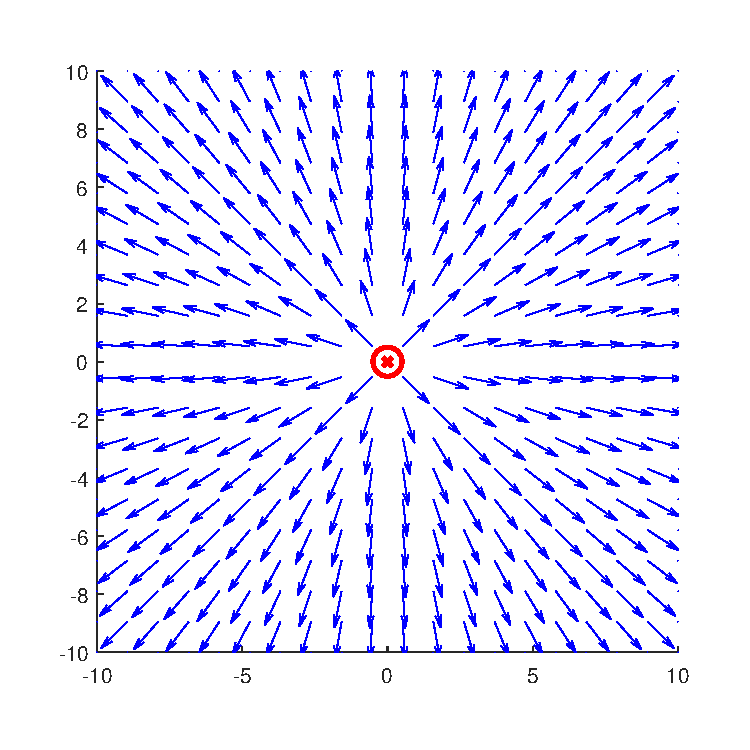
\includegraphics[width=6.5cm] {PaperFigures/compWithoutTitles/circRepulsiveSmallr}}
%		\hspace*{0mm}
%	\end{subfigmatrix}
%	\caption{Repulsive field with large path radius (a) and small radius (b)}
%	\label{fig:gvfRepulsiveRadius}
%\end{figure}
%
%The strength of the repulsive field was varied as a function of proximity $d$ by multiplying the repulsive field by a decay function $P$ bounded on the interval [-1,0], shown in Equation \ref{repulsiveDecay} and Figure \ref{fig:tanhICUAS2018}. The radius $R$ is the distance from the center of the field where vectors have effectively zero strength. 
%
%\begin{equation}
%P = R\frac{tanh(2\pi d-\pi)+1}{2}
%\label{repulsiveDecay}
%\end{equation}
%
%\begin{equation}
%\vec{v}_{repulsive} = -G||\vec{v_{conv}}||P
%\label{replulsiveField}
%\end{equation}
%
%
%
%\begin{figure}[H]
%	\begin{subfigmatrix}{2}% number of columns
%		\centering	
%		\subfigure []{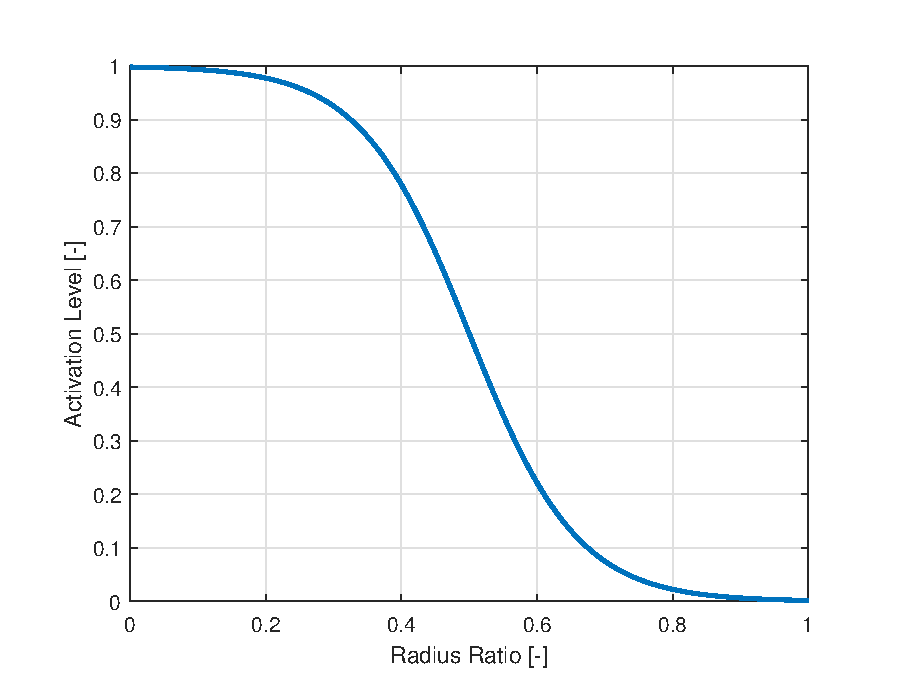
\includegraphics[width=8cm] {PaperFigures/tanh_ICUAS2018}}
%		\subfigure []{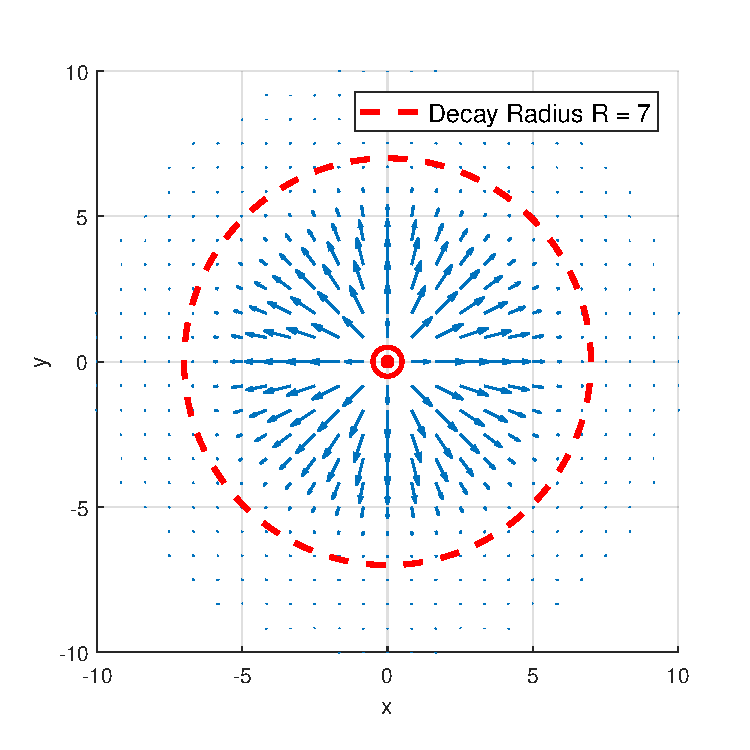
\includegraphics[width=7cm] {PaperFigures/repulsiveFields/circRepulsiveDecay}}
%		\hspace*{0mm}
%	\end{subfigmatrix}
%	\caption{Repulsive field activation \cite{wwc} (a) resulting repulsive field (b)}
%	\label{fig:tanhICUAS2018}
%\end{figure}
%
%
%Attractive and repulsive fields were added together similar to that in \cite{panagou_motion_2014} and the resulting vector shown in Equation \ref{summedAttRepulsive}. The resultant heading vector was used to guide a UAV to track a moving loiter circle while avoiding static obstacles, shown in Figure \ref{fig:gvfMovingTarget}.
%
%\begin{equation}
%\vec{V} = \vec{v}_{attractive}+\vec{v}_{repulsive}
%\label{summedAttRepulsive}
%\end{equation}
%
%
%
%\begin{figure}[h]
%	\centering
%	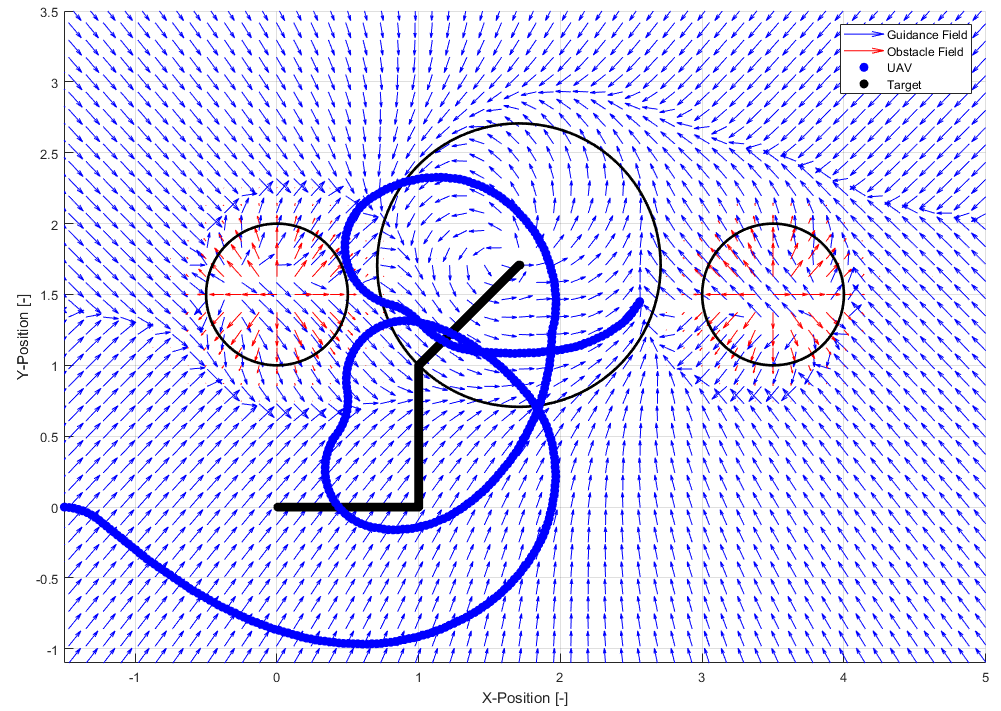
\includegraphics[width=10cm]{PaperFigures/gvfMovingTarget}
%	\caption{Place holder image of UAV following ground target \cite{wwc}}
%	\label{fig:gvfMovingTarget}
%\end{figure}
%
%
%GVF weights have been used for high level specification of the desired behavior for a UAV, whether it be for convergence, circulation, or avoidance. Repulsive GVFs have considered obstacle fields that strictly repel. The strictly repulsive guidance is effective at directing a UAV away from an obstacle, but provides no information on how to circumnavigate one. Additionally, further specification on the minimum radius and strength of the repulsive field may be useful in preventing a UAV from violating the obstacle circle. A preliminary simulation shows that a UAV encountering an obstacle while tracking a path may result in violation of the obstacle space, shown in Figure \ref{fig:singleobstacle}. UAVs traveling at lower velocities
% may also enter a trap situation where the guidance is confined to an infinite loop.
% \pagebreak
%
%\begin{figure}[h]
%	\centering
%	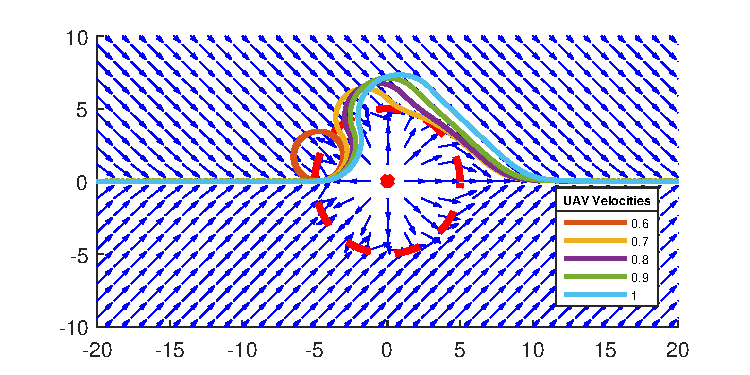
\includegraphics[width=12cm]{PaperFigures/singleObstacle}
%	\caption{Strictly repulsive obstacle on straight path}
%	\label{fig:singleobstacle}
%\end{figure}
%
%
%Adding circulation \textit{\textbf{H=1}} to the GVF in Figure \ref{fig:singleobstacle} prevented the trap situation for a velocity $u = 0.6$ and reduced the circumnavigation distance, which is shown in Figure \ref{fig:singleobstacleWithCirc}. Specifying vector field weights as functions of a UAV's state may enable an optimal guidance for obstacle avoidance. 
%
%\begin{figure}[h]
%	\centering
%	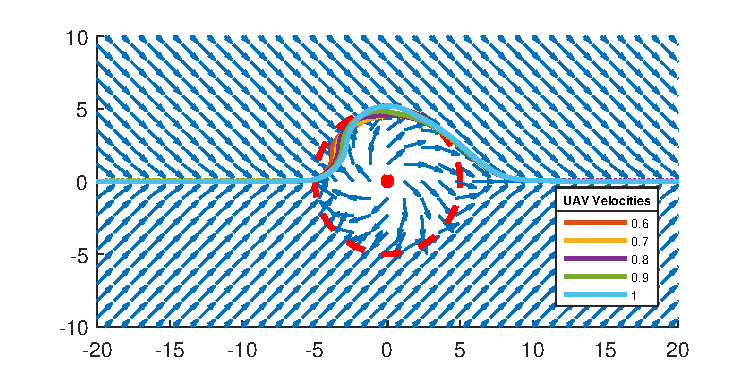
\includegraphics[width=12cm]{PaperFigures/singleObstacleWithCirc}
%	\caption{Circulating repulsive obstacle on straight path}
%	\label{fig:singleobstacleWithCirc}
%\end{figure}
%



%\pagebreak
%\section{Unmanned Aerial Vehicle Simulation}
%Testing new guidance, navigation, and control algorithms on flight hardware can be costly, require significant time, and requires an adequately large airspace. Before spending the time to reserve airspace and allocate man hours for flight tests it is important to test algorithms in a controlled environment. One way to accomplish testing without actual flight is through validation through mobile robots simulating fixed wing constraints \cite{ren_experimental_2007}, \cite{louali_designing_2014}, \cite{louali_experimental_2016}. Vector fields have been used in robot platforms other than UAVs, including ground \cite{kapitanyuk_guiding_2017} and marine \cite{schmitt_obstacle_2016}.
%
%\begin{figure}
%	\centering
%	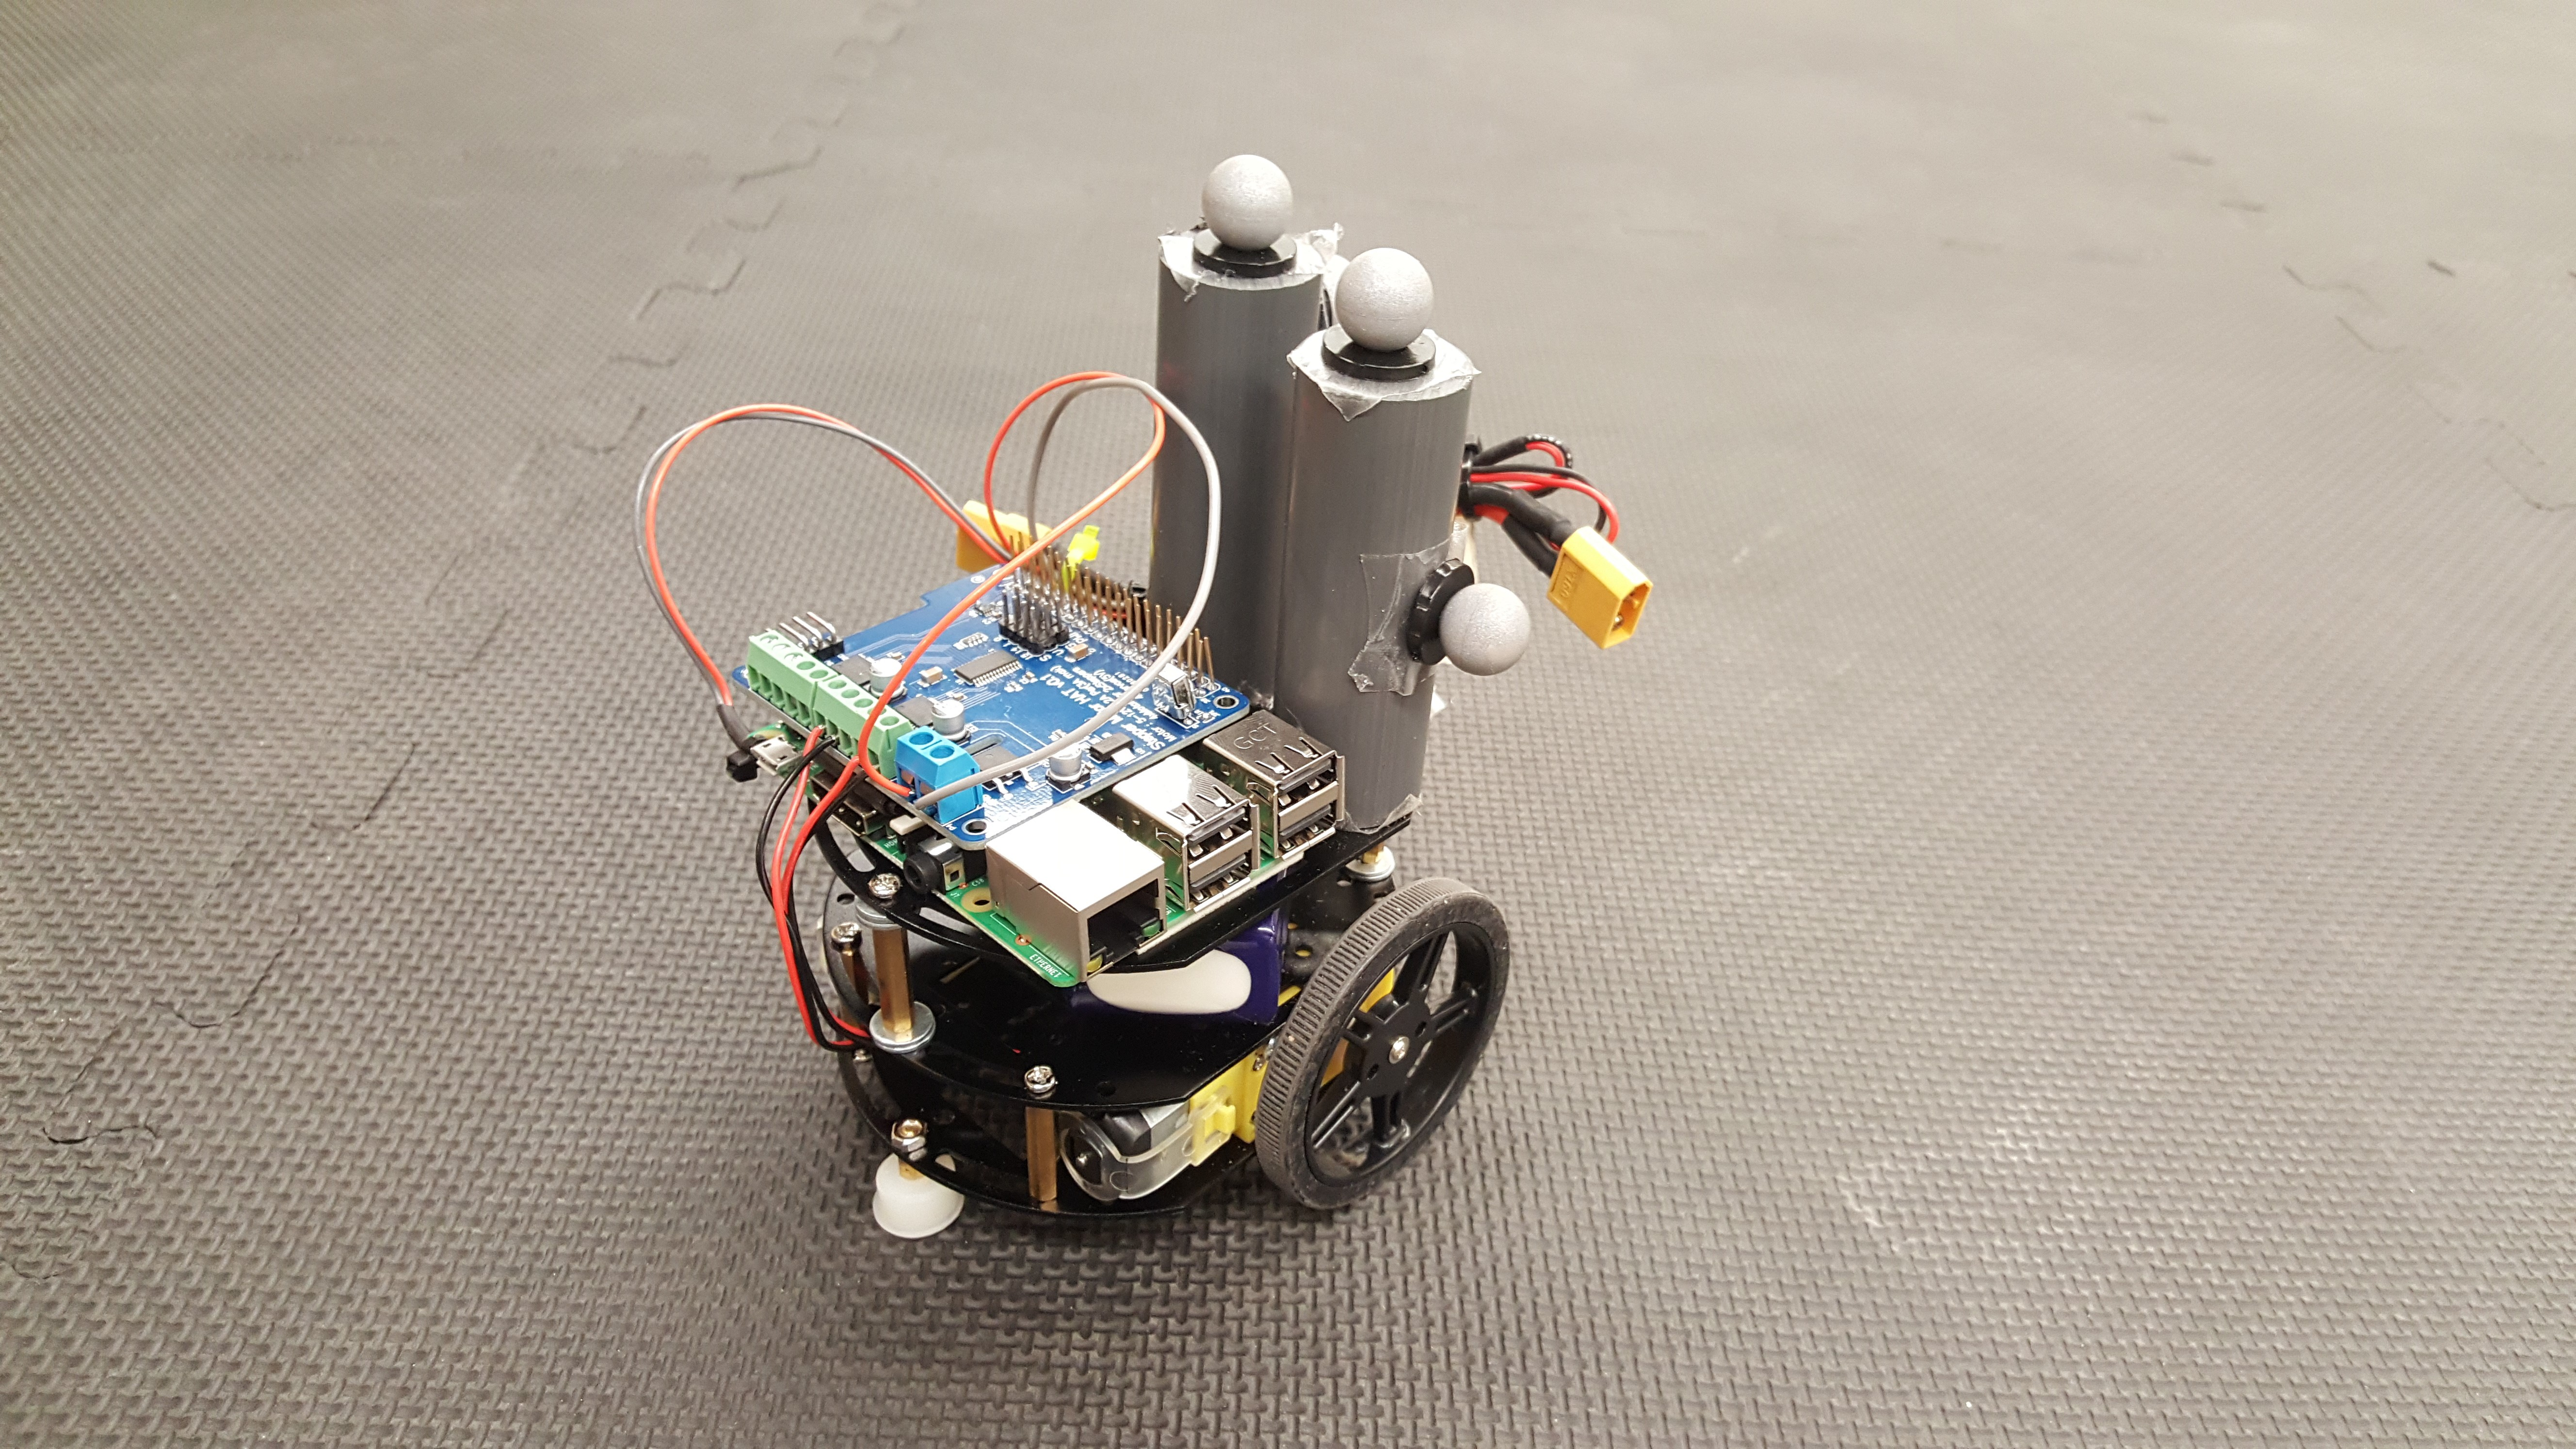
\includegraphics[width=15cm]{PaperFigures/robot}
%	\caption{Differential drive mobile robot simulating fixed wing UAV Dubins constraints}
%	\label{fig:robot}
%\end{figure}



\section{Introduction to Methodology}
A real-time circular obstacle avoidance guidance will be achieved by summing together a path following and obstacle avoidance vector field with optimized decay and circulation weights. Singularities in summed vector fields are defined and a method for numerically locating their position is presented in Phase I and it is shown how adding circulation to repulsive GVFs may remove singularities from the UAVs path. Phase II investigates a method for selecting the combination of repulsive GVF decay radius and circulation weights that minimizes a path deviation cost function. The optimized GVF guidance is implemented on an indoor multirotor UAV operating under fixed wing constraints in Phase III.


\section{Phase I: Gradient vector field singularity detection}
 \textbf{The objective of Phase I is to characterize and present a method for locating singularities in a summed gradient vector field.} Phase I consists of calculating guidance for converging and following a straight path using the GVF method in literature. A repulsive GVF is constructed for avoiding circular obstacles along the path by modifying the GVF's decay radius, convergence, and circulation weights. Summing the attractive and repulsive GVFs results in guidance that directs the UAV along the planned path while pushing away from the obstacle. Regions in the summed guidance where the path following and obstacle guidance directly oppose each other can result in vectors of zero length,called singularities. A method for identifying the location of singularities is presented along with a method for mitigating them. 
 

\subsection{Path Following Vector Field Guidance}
Guidance for converging and following a time-invariant path using GVF guidance is achieved by summing together convergence and circulation terms that are multiplied by scalars $G$ and $H$ respectively, shown in Equation \ref{simpleGVF}. The potential function $V$ in Equation \ref{potentialV} decreases asymptotically to null when approaching the target path and therefore the convergence vector begins to decrease as well \cite{goncalves_artificial_2009}. As the potential function decreases, the circulation term begins to dominate the guidance, promoting path following. How close to the target path the transition between convergence and circulation depends on the scalar weights $G$ and $H$ respectively. The total vector $\overrightarrow{V}_p$ represents the non-normalized attractive path following vector field comprised of both convergence and circulation terms. The shape of the target path that the vectors converge and follow depend on the specification of the implicit 3-dimensional surface functions $\alpha_1$ and $\alpha_2$. Intersecting two planes can be used to generate a GVF that converges and follows a straight path. The vertical plane, described in Equation \ref{eq:pathFunction}, at angle $\delta$ with respect to the paths $y-axis$, is intersected with a horizontal plane at constant height $z$, Equation \ref{eq:pathFunctionZ}



\begin{equation}
\label{eq:pathFunction}
\alpha_1 = cos(\delta)x + sin(\delta)y
\end{equation}

\begin{equation}
\label{eq:pathFunctionZ}
\alpha_2 = z
\end{equation}



\noindent
The gradient of the potential function, $\nabla V$, for calculating the path following convergence term is shown in Equation \ref{eq:potentialFunctionGrad}.

\begin{equation}
\label{eq:potentialFunctionGrad}
\nabla V = -\frac{1}{2(\sqrt{\cos^2(\delta) x^2+2\cos(\delta)\sin(\delta) xy +\sin^2 (\delta) y^2})} \begin{bmatrix}
2x\cos^2(\delta) + 2\cos(\delta)\sin(\delta) y \\
2y\sin^2(\delta) + 2\cos(\delta)\sin(\delta) x \\
2
\end{bmatrix}
\end{equation}

\noindent
Circulation is calculated by the cross product of the surface function gradients, which evaluates to that shown in Equation \ref{eq:circStraightPart2}.


\begin{equation}
\label{eq:circStraightPart2}
\overrightarrow{V}_{circ} = \begin{bmatrix}
sin(\delta) \\
-cos(\delta) \\
0
\end{bmatrix}
\end{equation}

The vector field $\overrightarrow{V}_p$ described will converge and circulate a straight path at the intersection of surfaces $\alpha_1$ and $\alpha_2$, depicted in Figure \ref{fig:planeIntersection}.

\begin{figure}[H]
	\centering
	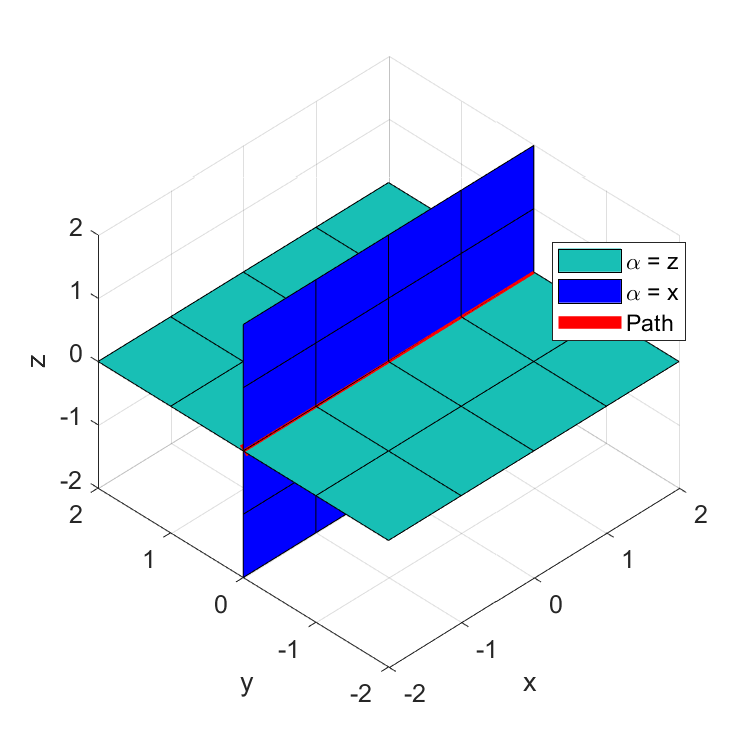
\includegraphics[width=8cm]{Figures/planeIntersection}
	\caption{Intersection of planes defined by implicit surface functions}
	\label{fig:planeIntersection}
\end{figure}

Prior to using the path following guidance $\overrightarrow{V}_p$, it is normalized, denoted as $\overrightarrow{V}_{||P||}$, to have a magnitude $||\overrightarrow{V}_p|| = 1$. The reason for normalizing the summed path following vector field is threefold. First, the vector is used as a heading controller only, therefore the angle of the vector is the information required by the autopilot. Second, the normalized vectors result in quiver plots with equal density arrows making the field easier to visualize. Lastly, normalizing the path following vector $\overrightarrow{V}_p$ fixes the length of the vector allowing for prediction of singularity location after summing the field, which will be discussed in the next section. Before discussing singularities, the obstacle field is introduced. 


\begin{equation}
% Component vector field with conv and circ
\overrightarrow{V}_{||P||} = \frac{\overrightarrow{V}_p}{||\overrightarrow{V}_p||}
\label{gonAllCompNormalized}
\end{equation}

To produce guidance for following a path and avoiding an obstacle, a repulsive obstacle vector field $\overrightarrow{V}_{||O||}$ needs to be constructed and summed with the normalized path following guidance $\overrightarrow{V}_{||P||}$. The repulsive vector field is multiplied by a decay function $P$ which limits the influence of the obstacle to a finite range and will be discussed after the avoidance field equations are presented. The sum of the two guidances is represented by $\overrightarrow{V}_g$ and is shown in Equation \ref{eq:totalGuidance}


\begin{equation}
\label{eq:totalGuidance}
\overrightarrow{V}_g = \overrightarrow{V}_{||P||} + P\overrightarrow{V}_{||O||}
\end{equation}

\noindent
Constructing the obstacle avoidance vector field $\overrightarrow{V}_{||O||}$ will now be discussed.

\subsection{Constructing an Avoidance Vector Field}

A circular avoidance vector field can be constructed in a way similar to that of the path following field in the previous section. What differentiates the obstacle field from the path following field is that the individual convergence $\overrightarrow{V}_{conv}$ and circulation $\overrightarrow{V}_{circ}$ components are normalized prior to summing to result in the obstacle field $\overrightarrow{V}_o$. The benefit of normalizing each field component before multiplying by their respective scalars $G$ and $H$ prior to summing is to produce an obstacle field with uniform behavior as distance from the obstacle increases. In short, normalizing each component allows both convergence and circulation terms to be present in the obstacle guidance at larger distances. Additionally, negative convergence weights will be used to produce vectors that diverge away from the path. The obstacle vector field is constructed using the normalized component Equation \ref{eq:obstComponents} with obstacle convergence and circulation weights $G_o$ and $H_o$ respectively.


\begin{equation}
% Component vector field with conv and circ
\overrightarrow{V}_{o} = G_o\frac{\overrightarrow{V}_{conv}}{||\overrightarrow{V}_{conv}||}+H_o\frac{\overrightarrow{V}_{circ}}{||\overrightarrow{V}_{circ}||}
\label{eq:obstComponents}
\end{equation}



A circular avoidance vector field with radius $r$ centered at $(x_c,y_c)$ is constructed by intersecting a cylinder, Equation \ref{eq:alphaCylinder}, and a plane Equation \ref{eq:pathFunctionZ}. 

\begin{equation}\label{eq:alphaCylinder}
\alpha_1 = (x-x_c)^2 + (y-y_c)^2-r^2
\end{equation}


Convergence is calculated by the gradient of the potential function \ref{eq:potentialFunctionGrad}, which when simplified evaluates to

\begin{equation}
\nabla V = A\overrightarrow{B}
\label{eq:AB}
\end{equation}

\noindent
where


\begin{equation}
A = \dfrac{-1}{\sqrt{\bar{x}^4+\bar{y}^4+2\bar{x}^2\bar{y}^2-2r^2\bar{x}^2-2r^2\bar{y}^2+r^2+z^2}}
\end{equation}

\begin{equation}
\overrightarrow{B} = \begin{bmatrix} 2\bar{x}^3+2\bar{x}\bar{y}^2-2r^2\bar{x} \\ 2\bar{y}^3+2\bar{x}^2\bar{y}-2r^2\bar{y} \\z \end{bmatrix}
\end{equation}

\noindent
and


\begin{equation}
\bar{x} = x - x_c
\end{equation}
\begin{equation}
\bar{y} = y - y_c
\end{equation}


Evaluating equation \ref{eq:AB} results in a vector field that converges to a circular path. Circulation is calculated from the cross product of each implicit surface function's gradient, which simplifies to



\begin{equation}
\label{eq:vcirc_circle}
\overrightarrow{V}_{circ} =  \begin{bmatrix}  2(y-y_c) \\[6pt] -2(x-x_c) \\[6pt] 0\end{bmatrix}
\end{equation}

The guidance $\overrightarrow{V}_o$ described by intersecting a cylinder and a plane can be shown in Figure \ref{fig:cylinderIntersection}. Note that repulsion from the path that lies at the intersection is achieved by a negative convergence weight, $G<0$.

\begin{figure}[H]
	\centering
	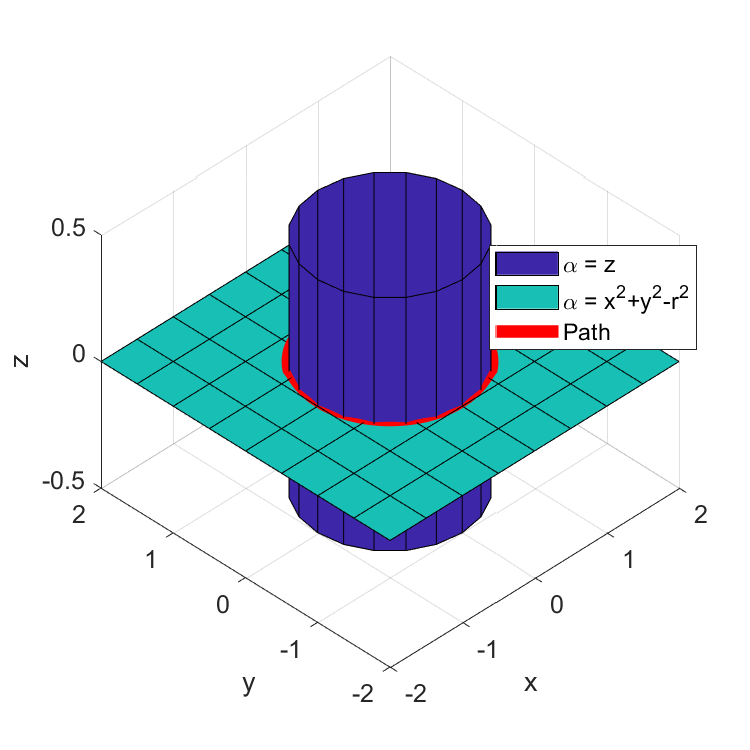
\includegraphics[width=10cm]{Figures/cylinderIntersection}
	\caption{Intersection of a cylinder and plane defined by implicit surface functions}
	\label{fig:cylinderIntersection}
\end{figure}

Obstacle fields should only act locally on a UAV guidance which is accomplished by applying a decay function for a field of radius $R$. The decay strength $P$ is determined in \ref{eq:decay}, where $d$ is the euclidean distance, or range, between the UAV and the center of the obstacle, shown in Equation \ref{eq:range}. At a distance $d>R$ the decay strength $P$ is effectively zero, having virtual no influence on the total guidance. At a distance $d\leq R$, the field strength is bounded between $[0,2]$. The selection of the decay function $P$ to be bounded as such is so that the obstacle field $\overrightarrow{V}_o$ eventually overpowers the path field $\overrightarrow{V}_{||P||}$. 


\begin{equation}
\label{eq:decay}
P = -\tanh \bigg( \frac{2\pi d}{R}-\pi\bigg)+1
\end{equation}

\begin{equation}
\label{eq:range}
d = \sqrt{ \bar{x}^2+\bar{y}^2}
\end{equation}


Prior to applying the decay function $P$ the obstacle field $\overrightarrow{V}_o$ is normalized. Forcing the obstacle guidance $\overrightarrow{V}_{||o||}$ to have unity magnitude, bounds the decayed guidance magnitude $P\overrightarrow{V}_{||o||}$ to the interval $[0,2]$ which allows a prediction of singularity location based on the range from obstacle center, $d$.


\begin{equation}
% Component vector field with conv and circ
\overrightarrow{V}_{||o||} = \frac{\overrightarrow{V}_{o}}{||\overrightarrow{V}_{o}||}
\label{eq:obstNormalized}
\end{equation}


\subsection{Summed Guidance and Singularity Definition}
The total summed guidance $\overrightarrow{V}_g$ defined in Equation \ref{eq:totalGuidance} can now be calculated and visualized, Figure \ref{fig:summedFieldsNoNorm}. In general, the GVF guidance is more easily visualized if the final guidance is normalized yet again, however, plotting the guidance $\overrightarrow{V}_g$ demonstrates regions where the fields oppose each other and decrease the total fields magnitude. For a strictly repulsive field that is centered on a straight path, regions of both constructive and destructive summation occurs. Note the vectors on the positive x-axis increasing in length as the two fields come together. Conversely, vectors in the negative x-axis show decreasing length and in some areas disappearing entirely.  

\begin{figure}[H]
	\centering
	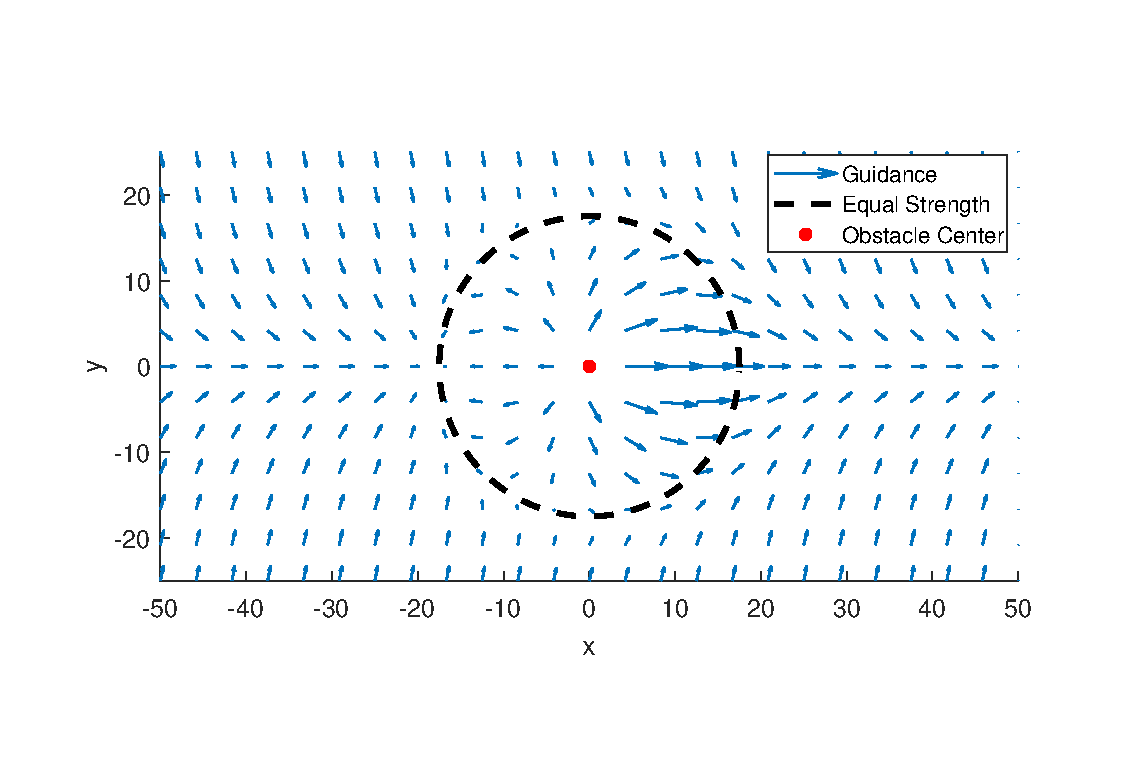
\includegraphics[trim=25 35 25 50,clip,width=14cm]{PaperFigures/Methods/summedFieldsNoNorm}
	\caption{Summed fields without total normalization $\protect \overrightarrow{V}_g$}
	\label{fig:summedFieldsNoNorm}
\end{figure}

Observing the regions around disappearing vectors it is shown that vectors appear to converge to a singular point from all direction, possibly indicating a trap situation. Visualizing the vector magnitudes of the scenario presented above can be accomplished with a summed field heat map, shown in Figure \ref{fig:summedHeatMap}, which shows the regions of decreasing magnitude more clearly. 


\begin{figure}[H]
	\centering
	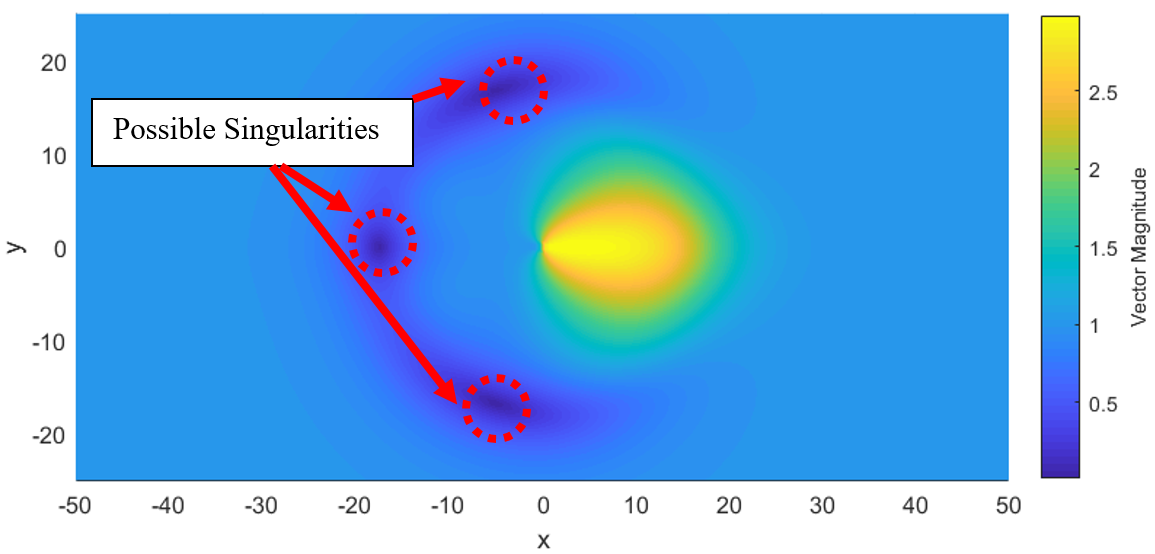
\includegraphics[trim=0 0 0 0,clip,width=14cm]{Figures/methods/summedHeatMapSimple2}
	\caption{Summed Fields Without Total Normalization}
	\label{fig:summedHeatMap}
\end{figure}

If singularities indicate possible trap situations, it is important to detect and avoid them. Singularities in the vector field are defined as a region in the GVF space where the vector has zero magnitude, shown in Equation \ref{eq:singularityCondition}.


\begin{equation}
\label{eq:singularityCondition}
||\overrightarrow{V}_g || = 0
\end{equation}

\noindent
By extension, singularities are a result of a zero vector, shown in Equation \ref{eq:zeroVectorCondition} and Equation \ref{eq:zeroVectorCondition2}.



\begin{equation}
\label{eq:zeroVectorCondition}
\overrightarrow{0} = \overrightarrow{V}_{||P||} +P\overrightarrow{V}_{||O||}
\end{equation}

\begin{equation}
\label{eq:zeroVectorCondition2}
\overrightarrow{V}_{||P||}=-P\overrightarrow{V}_{||O||}
\end{equation}

Vectors $\overrightarrow{V}_{||P||}$ and $\overrightarrow{V}_{||O||}$ are normalized, meaning that their magnitudes are of equal length $||\overrightarrow{V}_{||P||}||=||\overrightarrow{V}_{||O||}||$. For the condition shown in Equation \ref{eq:zeroVectorCondition2} to be true for an obstacle field with a negative convergence weight $G=-1$, the decay function $P$ must be unity. Setting Equation \ref{eq:decay} equal to $1$, the distance at which the fields have equal strength, and therefore possible singularity locations, is determined to be that shown in Equation \ref{eq:equalStrength}

\begin{equation}
\label{eq:equalStrength}
d = \frac{R}{2}
\end{equation}

Searching the GVF for locations that satisfy Equation \ref{eq:singularityCondition} can be accomplished numerically, however a good initial condition is necessary. Initial conditions placed at the radius of equal strength, defined by Equation \ref{eq:equalStrength}, on the side of the obstacle where deconstruction summation occurs the singularities can be found. Solving for the singularity locations with initial conditions placed evenly on the right hand side of the obstacle of the above scenario locates three singularities located on the radius of equation strength, shown in Figure \ref{fig:noCircSingularityDetection}.

\begin{figure}[H]
	\begin{subfigmatrix}{2}% number of columns
		\centering	
		\subfigure []{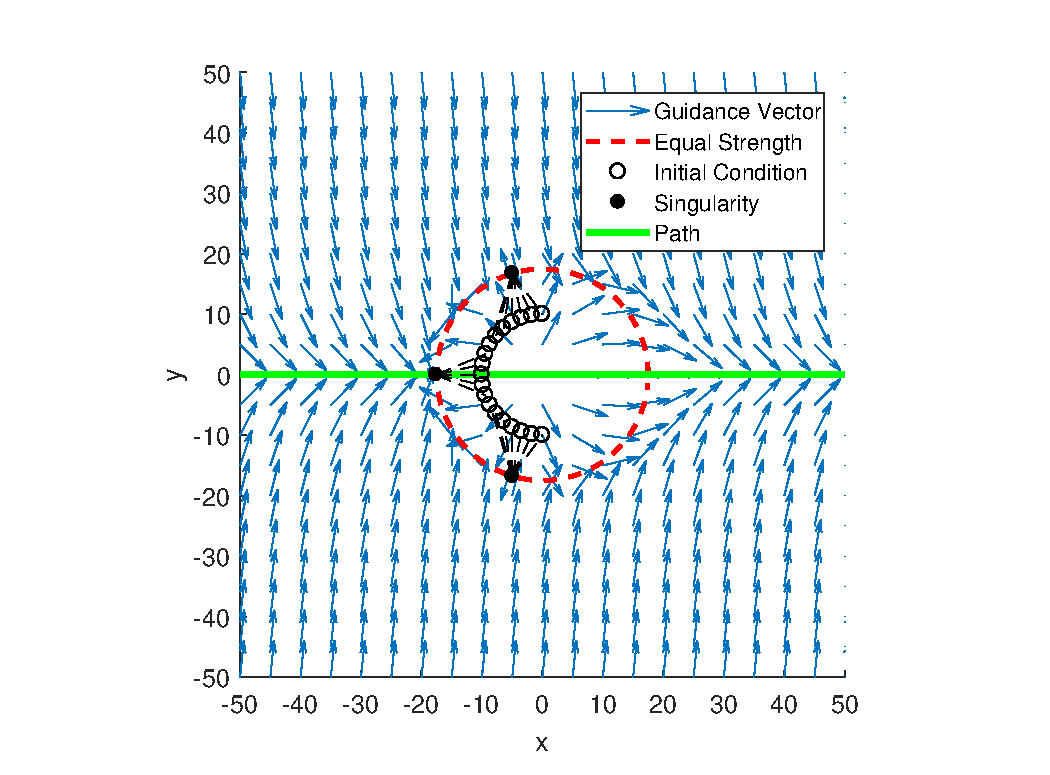
\includegraphics[trim=70 0 80 0,clip,width=7cm] {Figures/methods/noCircSingularityR10}}
		\subfigure []{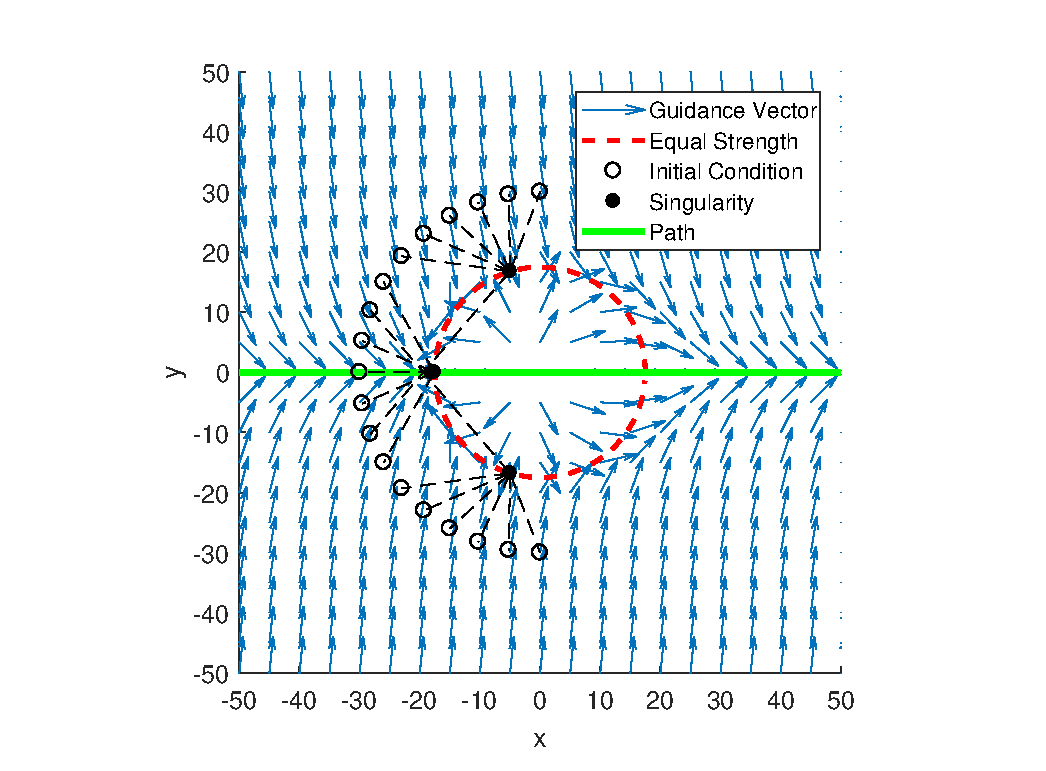
\includegraphics[trim=70 0 80 0,clip,width=7cm] {Figures/methods/noCircSingularityR30}}
		\hspace*{0mm}
	\end{subfigmatrix}
	\caption{GVF converging and circulating circular path}
	\label{fig:noCircSingularityDetection}
\end{figure}

By definition singularities are caused by the two vector fields directly opposing each other, described in Equation \ref{eq:zeroVectorCondition2}. Adding circulation to the repulsive GVF may prevent the summed vectors from canceling out completely. To demonstrate this, the above scenario is repeated with equal magnitude convergence and circulation components. Note that by adding circulation to the obstacle vector field, it prevents singularities from forming along the route the UAV is likely to take. Additionally, adding circulation provides a deterministic guidance on how to circumnavigate an obstacle. In literature, obstacles directed the UAV away and relied on the path following field for direction.
\hl{Generate (or find) figure with circulation added to show singularities removed from path}



\section{Phase II: Optimization of Obstacle Field}
\textbf{The objective of Phase II is to determine a combination of GVF circulation and decay radius for an optimized circular obstacle avoidance.} A demonstration of a UAV modeled as a Dubin's vehicle converging and following a straight path for various target path circulations is provided. A circular obstacle represented by a strictly repulsive GVF will be added to the path and the avoidance observed. Obstacles radius and their associated GVF decay radius will now be represented in terms of the UAVs turning radius for convenience. Next, a path deviation cost function is described and is to be minimized to provide an optimized GVF obstacle avoidance guidance. It is shown how cost is effected by modifying the decay radius and circulation for the worst-case obstacle avoidance scenario presented. Lastly, a method for solving for circulation and decay radius numerically is presented. 


\subsection{Vehicle and Obstacle Definition}

As discussed in literature and Phase I, GVF can be used to guide a UAV to get on and follow a path. An example of a UAV traveling at constant speed $u=20m/s$ and fixed turn rate $\dot{\theta}=20deg/s$ converging and circulating a straight path using the GVF guidance described in Phase I is shown in Figure \ref{fig:uavPathFollowDemo}. Starting at an initial position of $(-45,20)m$ and heading $\theta$ of $45^\circ$, the UAV is shown converging and following a straight GVF path with weights $G=1,H=5$.


\begin{figure}[H]
	\centering
	\includegraphics[trim=0 25 0 45,clip,width=14cm]{PaperFigures/Methods/uavPathFollowDemo}
	\caption{Fixed Wing converging and following a path}
	\label{fig:uavPathFollowDemo}
\end{figure}

The effect of modifying $G$ and $H$ has not been well documented in literature when the GVF is normalized for a heading guidance. To determine an appropriate relationship between circulation and UAV velocity, various path circulation weights for a fixed UAV velocity were conducted and the lateral error with respect to time recorded. As discussed in Phase I, increased circulation is expected to result in the vector field transitioning to path following more quickly. A low circulation weight allows convergence to dominate closer to the path. The UAVs route for converging and following a path with $G=1$ and multiple path circulation weights $H$ is shown in Figure \ref{fig:uavPathMultipleHs}. As expected, a low circulation results in a UAV route that quickly approaches the path, however begins to oscillate and has a larger stead-state error compared to larger circulation fields. The largest circulation field $H=50$, does not oscillate, but takes considerably longer to converge. Circulation approximately the same value as the UAV's velocity results in a compromise between fast convergence and no oscillation. The lateral error from the path is shown in Figure \ref{fig:uavPathMultipleHsLateral}. 


\begin{figure}[H]
	\centering
	\includegraphics[trim=0 30 0 65,clip,width=14cm]{PaperFigures/Methods/pathMultipleHs}
	\caption{Fixed Wing converging and following a path}
	\label{fig:uavPathMultipleHs}
\end{figure}


\begin{figure}[H]
	\centering
	\includegraphics[trim=0 0 0 0,clip,width=16cm]{PaperFigures/Methods/lateralErrorVsTime}
	\caption{Lateral error for fixed wing guided by GVF guidance of multiple circulations}
	\label{fig:uavPathMultipleHsLateral}
\end{figure}

From the above simulation it is observed that a circulation near the UAVs velocity provides a flight route that is in-between the high oscillation and high overshoot of a circulation $H=1$ while not having a longer settling time with high circulation $H=50$. For future simulations the circulation of the path following guidance will be assumed to be equal to that of the UAVs velocity, $H=u$. \\

As the UAV travels the path using GVF guidance, an obstacle may be encountered that, without intervention, the UAV will collide with. Obstacles along the pre-planned path are described using two parameters, the obstacle radius $r_o$ and the lateral distance from the path $y_o$. Representing the obstacle's position with respect to the path is useful because it allows for a single optimized GVF solution to be applicable for multiple path angles $\delta$.

\begin{figure}[H]
	\centering
	\includegraphics[width=14cm]{Figures/methods/obstacleOnPath}
	\caption{Circular obstacle along planned path}
	\label{fig:obstacleonpath}
\end{figure}

 It is assumed here that the radius of the obstacle is no smaller than the turn radius of the UAV $\theta_r$, which is calculated in Equation \ref{eq:turning_radius}. It is convenient to represent the obstacle's radius as $m$ multiples of the UAV's turning radius, shown in  Equation \ref{eq:obstR}.
 


\begin{equation}
\label{eq:turning_radius}
\theta_r = \frac{u}{\dot{\theta}}
\end{equation}

\begin{equation}
\label{eq:obstR}
r_o = m \theta_r
\end{equation}

 The repulsive vector field's decay radius $R$ is defined in $k$ multiples of the obstacle's radius, shown in Equation \ref{eq:decayR}. 
 
 \begin{equation}
 \label{eq:decayR}
 R = k r_o
 \end{equation}
 
 

 A cost function can be used to measure the deviation from a planned path while avoiding an obstacle with GVF in Equation \ref{eq:staticCost}. The deviation, y, is the lateral distance of the UAV to the planned path, $R$ is the obstacle radius.
 
 \begin{equation}
 \label{eq:staticCost}
 \gamma = \frac{1}{r_o}\int_{0}^{tf}ydt
 \end{equation}
 
 
 Strictly repulsive GVF obstacle fields can provide avoidance, however may cause excess deviation from the pre-planned path, cause unnecessary turns, and flight routes near or through guidance singularities. A UAV traveling at a speed of $10m/s$ and a turn rate of $20 deg/s$ is given a summed path following and obstacle avoidance guidance $\overrightarrow{V}_g$, defined in Equation \ref{eq:totalGuidance} in Phase I. An obstacle centered on the path $y_o=0$ and radius $r_0 = \theta_r$ is to be avoided. The decay radius multiplier $k$ was increased manually over several simulations until avoidance was achieved. The flight path of the UAV flying with summed guidance is shown in Figure \ref{fig:uavPathObstNoCirc}. The UAV experiences excessive path deviation and takes considerable time to settle back to the planned path. Additionally, the guidance directs the UAV to pass directly through a singularity and passes near an additional singularity towards the top of the obstacle. The cost, calculated from Equation \ref{eq:staticCost}, for avoidance using the strictly repulsive guidance for head on collision scenario is $\gamma=25$.
 

\begin{figure}[H]
	\centering
	%Simulations performed with findSingularities.m
	%G=-1,H=0, n = 1.5,k=2.8
	\includegraphics[trim=0 85 0 85,clip,width=15cm]{PaperFigures/Methods/bruteForceSolveN1V10}
	\caption{UAV encountering a circular obstacle centered on pre-planned path, no circulation}
	\label{fig:uavPathObstNoCirc}
\end{figure}

Adding circulation to the obstacle guidance $\overrightarrow{V}_o$, as described in Phase I, may remove singularities from the UAVs route. Additionally, circulation adds deterministic information on how to circumnavigate an obstacle whereas strictly repulsive fields rely on the path following field to determine circumnavigation direction. Equal magnitudes convergence $G_o$ and circulation $H_o$ removes the guidance singularities from the UAV's path, adds a more gentle transition between fields, and guides the UAV back to the planned path more quickly, shown in Figure\ref{fig:uavPathObstWithCirc}. The cost of the head on collision avoidance using GVF guidance with obstacle circulation results in a cost of $\gamma=7$.



\begin{figure}[H]
	\centering
	\includegraphics[trim=0 85 0 85,clip,width=15cm]{PaperFigures/Methods/bruteForceSolvedN1V10WithCirc}
	\caption{UAV encountering a circular obstacle centered on pre-planned path with circulation}
	\label{fig:uavPathObstWithCirc}
\end{figure}

Adding equal parts $G$ and $H$ produce guidance with a lower cost compared to strictly repulsive, however, $k$ and $H$ should be selected such that the cost is minimized. One method for selecting what these field parameters should be is to evaluate a large range of parameters and observe the cost for avoidance with each combination. The cost function shown in Equation \ref{eq:staticCost} only penalized the UAV for path deviation, however should be modified to also be penalized for violating the obstacle space. The new cost function $\bar{\gamma}$ adds an additional piecewise function which increases the cost if the UAV is inside or on the obstacle's edge, shown in Equation \ref{eq:staticCostWithObst}


 \begin{equation}
\label{eq:staticCostWithObst}
\bar{\gamma} = \frac{1}{r_o}\int_{0}^{tf}ydt + j(x,y)
\end{equation}

\begin{equation}
j(x,y) = \left\{
\begin{array}{ll}
100dt & \quad \sqrt{(x-xc)^2+(y-yc)^2} \leq r_O \\
0 & \quad \sqrt{ (x-xc)^2+(y-yc)^2 } > r_O
\end{array}
\right.
\end{equation}


Using the above cost function $\bar{\gamma}$ in the same scenario presented in Figure \ref{fig:uavPathObstNoCirc}, several simulations were conducted with identical UAV parameters and obstacle radius $r_o$ with varying $k$ and $H_o$ values. The cost of each simulation is shown in the heatmap in Figure \ref{fig:costHandR}. 

\begin{figure}[H]
	\centering
	\includegraphics[trim=0 0 0 10,clip,width=16cm]{PaperFigures/Methods/costHandR.png}
	\caption{Heatmap of cost as function of $k$ and $H_o$}
	\label{fig:costHandR}
\end{figure}

Finding the minimum cost of the above heatmap and looking up the corresponding $k$ and $H_o$ values at which the minimum occurs can be used to provide an optimized avoidance. Solving the desired parameters for an optimal guidance using this search method for the general case is computationally expensive and can take many hundreds of simulations to evaluate the desired space. The problem becomes one of minimization of the cost function and to find a solution numerically without solving for a large range of parameters, shown in Equation \ref{eq:minimizer}.

\begin{equation}
\label{eq:minimizer}
\begin{aligned}
& \underset{H,k}{\text{minimize}}
& & \frac{1}{R}\int_{0}^{tf}ydt + j(x,y) 
\end{aligned}
\end{equation}

A numerical solver which attempts to minimize a given cost function can be found in MATLAB called $fmincon()$. The minimizer operates on the following principle. Provided an initial condition array $X_I$, minimize the function $\bar{\gamma}$ by observing the change in $\bar{\gamma}$ within certain bounds. Using the minimizer method a solution to the above problem of a UAV following a path with a head-on collision scenario with an obstacle was found in 5.2 seconds compared to [insert time for finding solution with heat map]. The reduction in cost as the minimizer runs is shown in Figure \ref{fig:finalfunctionvalue}.

\begin{figure}[H]
	\centering
	\includegraphics[width=12cm]{PaperFigures/Methods/finalFunctionValue}
	\caption{Cost function reduction in fmincon()}
	\label{fig:finalfunctionvalue}
\end{figure}

The optimizer found a solution combination of $k=2.7$ and $H_o = 1.8$ and results in a path with cost $\bar{\gamma}=14$. The path can be seen below in Figure \ref{fig:optimizedPath}. \hl{Discuss the percent difference from all the methods, possibly make a table discussing the computation time}

\begin{figure}[H]
	\centering
	\includegraphics[trim=0 85 0 85,clip,width=15cmm]{PaperFigures/Methods/solvedN1V10}
	\caption{UAV path from optimized GVF}
	\label{fig:optimizedPath}
\end{figure}

The optimized GVF guidance was shown to provide an improved guidance with a reduced path deviation compared to standard GVF guidance. Determining how GVF compares against other methods such as VFF, waypoint, and the optimal path around an obstacle is now discussed. 


%The optimized GVF guidance was shown to provide a route for the UAV with lower deviation compared to the non-optimized GVF for a worst case head on collision scenario. GVF will be compared against potential field, waypoint guidance, and the optimal avoidance route. 


\subsection{Optimal Avoidance Route for Straight Path}
A geometrically optimal route around a circular obstacle can be used to compare the performance of avoidance algorithms. The path for avoiding a circular obstacle while minimizing path deviation can be accomplished with three circular arc turns. The first and third arc utilize the UAVs minimum turning radius, $\theta_r$, calculated in Equation \ref{eq:turnRadius}. The start of the first minimum radius turn begins when the UAV's horizontal position $x$ reaches  $\tilde{x}$ from the path frame origin. At a horizontal position $-\hat{x}$ the UAV turns with a radius of the obstacle $r_o$ and exits when the UAVs horizontal position reaches $\hat{x}$. 

\begin{equation}
\label{eq:turnRadius}
\theta_r = \frac{u}{\dot{\theta}}
\end{equation}

\noindent
The horizontal points $\tilde{x}$ and $\hat{x}$ are shown in Equations \ref{eq:optPathXtilde} and \ref{eq:optPathXhat} respectively. 

\begin{equation}
\label{eq:optPathXtilde}
\widetilde{x} = -\sqrt{(\theta_r+R)^2 - (\theta_r-Y_o)^2}
\end{equation}

\begin{equation}
\label{eq:optPathXhat}
\hat{x} = \frac{R\sqrt{(r+R)^2-(\theta_r-Y_o)^2}}{R+\theta_r}
\end{equation}

\noindent
The avoidance path for navigating around a circular obstacle with maximum coverage of a sensor line is defined in Equation \ref{eq:optPath} and shown in Figure \ref{fig:optimalpath}.


\begin{equation}
\label{eq:optPath}
y(x) = \left\{
\begin{array}{ll}
\widetilde{y} -\sqrt{\theta_r^2 - (x-\widetilde{x})^2} &  x < -\hat{x} \\
Y_o +\sqrt{R^2 - x^2} & -\hat{x} \leq x \geq \hat{x}\\
\widetilde{y} -\sqrt{\theta_r^2 - (x+\widetilde{x})^2}&  x > -\hat{x}
\end{array}
\right.
\end{equation}

\begin{figure}[H]
	\centering
	\includegraphics[width=0.7\linewidth ,trim=0 265 0 20,clip,width=15cm]{Figures/optimalPath/optimalPath}
	\caption{Optimal Kinematic Path Around Circular Obstacle}
	\label{fig:optimalpath}
\end{figure}

The avoidance path represents the optimal path around a circular obstacle and would be used to generate waypoints for waypoint guidance.

\subsection{Optimal Avoidance Path and Waypoints}

 The number of waypoints that divert around an obstacle effects how closely the UAV tracks the outside of the obstacle and how much of the original path can be traveled. Few obstacle diversion waypoints leads to excess path deviation while increasing the number of diversion waypoints reduces path deviation, however has diminishing returns. The cost function in Equation \ref{eq:staticCost} is used below to demonstrate how increasing the number of waypoints decreases the cost function, however approaches an asymptote around six waypoints.


\begin{figure}[H]
	\begin{subfigmatrix}{2}% number of columns
		\centering	
		\subfigure []{\includegraphics[width=7.5cm,trim=40 0 50 0,clip] {Figures/Waypoints/1Wpts}}
		\subfigure []{\includegraphics[width=7.5cm,trim=40 0 50 0,clip] {Figures/Waypoints/6Wpts}}
		\hspace*{0mm}
	\end{subfigmatrix}
	\caption{Obstacle Diversion Waypoints}
	\label{fig:numWaypointsPath}
\end{figure}

\begin{figure}[H]
	\centering
	\includegraphics[width=10cm]{Figures/Waypoints/costVnumWpts}
	\caption{Cost impact versus number of waypoints}
	\label{fig:numWaypoints}
\end{figure}



\subsection{Worst Case Avoidance Scenario}
A worst case avoidance scenario will be used to compare the optimized GVF with waypoint, VFF, and the optimal path with respect to the path deviation cost function. A circular obstacle centered on the path, $y_o = 0$, requires a deviation from the path of at least $50\% $ of the obstacles radius. A fixed wing UAV at an initial position $(-400,0)$ and heading $\theta=0^\circ$ follows the straight path connecting the points $(-400,0)$ and $(400,0)$ respectively. Traveling at a constant speed $u=25 m/s$ and with a fixed turn rate of $\dot{\theta}=20 deg/s$ the UAV must avoid an obstacle with radius $2\theta_r$ located at the origin $(0,0)$. The VFF guidance from \cite{borenstein_real-time_1990} is used with an obstacle window radius of $\theta_r+r_o$, a cell repulsion $Fr=-3$, attraction force $F_t=0.8$, range exponent $n=2$, and a goal located at $(700,0)$. For LOS waypoint guidance, $7$ waypoints with a small waypoint radius of $10m$ was chosen. Each diversion waypoint added drives the guidance closer to optimal, however has diminishing returns past $6-7$ waypoints. GVF guidance with a circular repulsive field was assigned a convergence weight $G=-1$ and circulation and decay radius coefficient $k$ were determined by evaluating the cost function in Equation \ref{eq:staticCost} with initial conditions $k_i = 2$ and $H=2$. The GVF solution was bounded such that $2\leq k\leq 4$ and $1\leq H\leq 6$.  Minimizing the cost function resulted in a decay radius coefficient $k=2.78$ and a circulation value $H=1.88$. The Dubin's paths for the three guidance methods discussed is shown in Figure \ref{fig:comparemethods}. \\

VFF results in a UAV route that has excess deviation from the planned path with excessive turns. Waypoint guidance returns to the path more quickly than VFF, however deviates from the planned path farther then necessary. GVF leaves the path before waypoint guidance and tracks the outside of the obstacle closely and then quickly converges back to the pre-planned path. The cost of each method, defined in Equation \ref{eq:staticCost}, is displayed in the bar plot shown in Figure \ref{fig:barplotperformance}.


\begin{figure}[H]
	\centering
	\includegraphics[trim=0 50 0 65,clip,width=15cm]{Figures/Simulations/compareMethods}
	\caption{Path of UAV guided by guidance methods}
	\label{fig:comparemethods}
\end{figure}


\begin{figure}[H]
	\centering
	\label{fig:barPlotCost}
	\includegraphics[width=15cm]{Figures/Simulations/barPlotPerformance}
	\caption{Cost performance for various UAV guidance methods}
	\label{fig:barplotperformance}
\end{figure}





\section{Phase III}
\textbf{The objective of Phase III is to demonstrate the optimized gradient vector field guidance presented in Phase II on multirotor UAV flying with fixed wing turn-rate constraints.} A description of the experimental setup will be given for both the hardware and software that was implemented to achieve GVF guidance. An overview of the validation of a conversion to python from MATLAB is discussed. Lastly a description of an avoidance scenario is presented.


\subsection{Experimental Overview}
All of the scenarios discussed using GVF guidance have involved simulating a fixed wing UAV modeled as a Dubin's vehicle. To demonstrate the GVF on actual flight hardware, an indoor quadcopter, Figure \ref{fig:crazyflie2}, will be used in place of a fixed wing UAV. There are several reasons why using an indoor quadcopter is advantageous for experimental flight tests, such as new guidance systems. First, finding an airspace to safely test the guidance system with an adequate clearing for takeoff and landing can be difficult. Many environmental complications such as high winds, precipitation, and low visibility could delay or prevent flight tests all together. Testing the GVF guidance method on an indoor quadcopter remove these complications. Additionally, the Dubin's turn rate constrains can be applied to limit the maneuverability of the quadcopter so that it behaves similar to that of a fixed wing UAV. Flying indoors also allows for more repeatable experimentation, environmental control, and use of high speed motion capture systems to provide position information to guidance and control systems. 



\begin{figure}
	\centering
	\includegraphics[trim=0 25 0 30,clip,width=7cm]{PaperFigures/crazyflie}
	\caption{Micro quadcopter Crazyflie 2.0 by bitcraze}
	\label{fig:crazyflie2}
\end{figure}


The micro quadcopter, crazyflie 2.0, designed by Bitcraze was selected as the experimental flight vehicle due to its low cost and the ability to send the vehicle roll rate, pitch rate, yaw, and thrust commands directly over radio. The control messages can be sent through the object oriented and scripted language Python, a language with syntax very similar to MATLAB. The UAV was viewed by 8 vicon vero cameras detect infrared light reflected by small markers placed on the vehicle. Video captured by the cameras at 100Hz is sent to a PC with a software package that estimates the pose of the vehicle and sends that information over a local area network (LAN) to a ground station PC where guidance and control calculations are made. The command messages are then sent over radio to the crazyflie where an on-board controller accepts the commands and outputs the necessary motor output to achieve the commands. A high level overview of the experimental framework described is shown in Figure \ref{fig:experimentalFramework}. Each component of the framework will be discussed in more detail in the proceeding sections. 

\begin{figure}
	\centering
	\includegraphics[trim=0 0 0 0,clip,width=15cm]{PaperFigures/Methods/experimentalSetup}
	\caption{Indoor quadcopter flight experimental layout}
	\label{fig:experimentalFramework}
\end{figure}

\subsection{Crazyflie 2.0}
The crazieflie 2.0 is a lightweight micro-quadcopter UAV weighing in at 27 grams and has an approximate payload capacity of 10 grams. An on-board flight controller maintains vehicle stability by estimating it's attitude and making corrections to the four brushed motors. One of the conveniences of the crazyflie 2.0 is the ability to send roll rate, pitch rate, yaw, and thrust over radio in order to control the UAV directly. The software package, cfClient, interfaces with the crazyflie to accept and transmits these control messages over radio. 


\begin{figure}[H]
	\centering
	\includegraphics[trim=0 0 0 0,clip,width=12cm]{PaperFigures/Methods/cfClient}
	\caption{Crazieflie client radio communication software}
	\label{fig:cfClient}
\end{figure}

The guidance and control software that calculates these command messages was hosted on a remote machine and not on-board the UAV, primarily for the convenience of fast development. The guidance and control was written in Python, which is highly portable and could easily be implemented on-board a UAV. 

%\subsection{Vicon Motion Capture}
%
%\begin{figure}
%	\centering
%	\includegraphics[trim=20 100 100 100,clip,width=12cm]{PaperFigures/Methods/viconObject}
%	\caption{Indoor quadcopter flight experimental layout}
%	\label{fig:viconObject}
%\end{figure}
%
%\begin{figure}[H]
%	\centering
%	\includegraphics[trim=0 0 0 0,clip,width=14cm]{PaperFigures/Methods/viconArea}
%	\caption{\hl{TEMPORARY VICON AREA PHOTO}}
%	\label{fig:cfControlClass}
%\end{figure}
%



\subsection{Python Guidance and Control Ground Station}

The guidance and control framework developed for experimentation resembles that described in Figure \ref{fig:autopilotloops}. A navigation script taps into a stream of data provided by the Vicon tracker software and distributes that data to guidance and control algorithms. Position $(x,y,z)$ and yaw $\phi$ are provided to the control algorithm which consists of four PID controllers. The UAV was set to fly at constant altitude for all simulations and experimentation, therefore only planar position $(x,y)$ were provided to the guidance system. Heading guidance from the optimized GVF was converted to a carrot located at a position $(xc,yc)$ is sent to the control system to be used as set-points. Control messages are relayed to a radio interface software, cfClient, which communicates the control messages with the crazyflie. An overview of the described system is shown in Figure \ref{fig:cfControlClass}.

\begin{figure}[H]
	\centering
	\includegraphics[trim=0 0 1 0,clip,width=14cm]{PaperFigures/Methods/cfControlClass}
	\caption{Crazyflie Guidance and Control Software Framework}
	\label{fig:cfControlClass}
\end{figure}

The control algorithm consists of four PID controllers which are used to calculate roll rate, pitch rate, yaw, and thrust to drive the UAV to a desired setpoint. The error is measured by subtracting the measured state $(x,y,z,yaw)$ from the desired setpoint. The block diagram of the PID controller is shown in Figure \ref{fig:pid}. Gains P, I, and D for each controller is tabulated in Table \ref{table:pidGains} below. 



\begin{figure}[H]
	\centering
	\includegraphics[trim=0 0 0 0,clip,width=14cm]{PaperFigures/Methods/pid}
	\caption{Crazyflie Guidance and Control Software Framework}
	\label{fig:pid}
\end{figure}

\begin{table}[H]
	\centering
	\caption{Tuned PID gains for roll, pitch, yaw, and thrust controller}
	\label{table:pidGains}
	\begin{tabular}{|c|c|c|c|}
		\hline 
		Control Parameter & P & I & D \\ 
		\hline 
		Roll Rate & 29 & 2.5 & 19 \\ 
		\hline 
		Pitch Rate & 29 & 2.5 & 19 \\ 
		\hline 
		Yaw & 80 & 50 & 30 \\ 
		\hline 
		Thrust & 100 & 90 & 70 \\ 
		\hline 
	\end{tabular}
\end{table}
 

The optimized GVF guidance developed in MATLAB in Phases I and II was programmed into Python and compared under several scenarios to ensure that the methods were identical. First, a path following GVF was calculated in Python for a straight line and results overlaid with an identical scenario in MATLAB. The quiver plots show guidance calculated by MATLAB aligning with the guidance calculated in Python shown in Figure \ref{fig:valPythonStraightPath}.



\begin{figure}[H]
	\centering
	\includegraphics[trim=0 150 0 150,clip,width=10cm]{PaperFigures/Methods/resultsPython/PathConfirm}
	\caption{Validation of Python straight path guidance overlaid with MATLAB}
	\label{fig:valPythonStraightPath}
\end{figure}

Validating for an avoidance field with equal parts circulation and repulsion are shown in Figure \ref{fig:valPythonAvoidance}


\begin{figure}
	\centering
	\includegraphics[trim=0 140 0 140,clip,width=10cm]{PaperFigures/Methods/resultsPython/obstacle}
	\caption{Validation of Python obstacle guidance overlaid with MATLAB}
	\label{fig:valPythonAvoidance}
\end{figure}

Avoidance field with the decay applied in Figure \ref{fig:valPythonAvoidanceDecay}

\begin{figure}[H]
	\centering
	\includegraphics[trim=0 140 0 140,clip,width=10cm]{PaperFigures/Methods/resultsPython/obstacleWithDecayAndCirculation}
	\caption{Validation of Python obstacle decay guidance overlaid with MATLAB}
	\label{fig:valPythonAvoidanceDecay}
\end{figure}

Summed path following and obstacle avoidance guidance with an obstacle field with no circulation is shown in Figure \ref{fig:valPythonSummed}.

\begin{figure}[H]
	\centering
	\includegraphics[trim=0 140 0 140,clip,width=10cm]{PaperFigures/Methods/resultsPython/summedFields}
	\caption{Validation of Python summed guidance overlaid with MATLAB}
	\label{fig:valPythonSummed}
\end{figure}

Lastly, the Python guidance was simulated with an identical Dubins vehicle as MATLAB and compared in Figure \ref{fig:pythonMATDubins}

\begin{figure}[H]
	\centering
	\includegraphics[trim=0 230 0 260,clip,width=16cm]{PaperFigures/Methods/resultsPython/dubinsPaths}
	\caption{Validation of Python Dubins UAV route overlaid with MATLAB}
	\label{fig:pythonMATDubins}
\end{figure}



\section{Summary of Methodology}

Equations for path following and obstacle vector field guidance were presented. Singularities in a summed field were discussed and a method for locating them numerically was provided. A Dubin's UAV modeled representing a fixed wing UAV kinematics guided by a path following guidance is presented. Obstacles were defined in terms of UAV turning radius for convenience. Cost functions for evaluating the performance of obstacle avoidance in terms of path deviation was provided. Paths with strictly repulsive guidance were shown to guide UAV away from the obstacle but with excess path deviation, unnecessary turns, and slow path convergence. Adding circulation to the obstacle field improved performance and reduced the overall cost. A large space of circulation and decay multipliers were evaluated and the cost displayed in a heatmap. The combination of parameters that provide the least cost guidance can be selected to provide an optimized guidance, however takes significant computation time to evaluate the large parameter space. A numerical method for determining parameters was presented and an example of it's execution provided. Lastly, the optimized GVF guidance was implemented into python to be used for real-time obstacle avoidance guidance for the crazyflie quadcopter. Next, results for each phase will be discussed. 


\chapter{Results}
\section{Introduction to Results}
\hl{fill out}

\section{Phase I \& II}

The methods discussed in Phase I and Phase II for detecting singularities in a GVF and optimizing obstacle field decay radius and circulation will now be demonstrated for several scenarios involving a fixed wing UAV. Avoidance scenarios that represent the possible configurations of an obstacle that lies along a pre-planned path consist of small obstacles, large obstacles, path centered obstacles, and path offset obstacles. small obstacles are considered those with radius $r_o = \theta_r$ while large obstacles have a radius $r_o\ge5\theta_r$. Centered obstacles represent the worst case avoidance scenario where the UAV must deviate at least $50\%$ of the obstacles radius in order to successfully avoid. For the path centered obstacle, counterclockwise and clockwise avoidance have identical costs. In the centered obstacle scenarios presented, it is assumed that clockwise avoidance is desired and the initial conditions and bounds are set accordingly. A table of the avoidance scenarios demonstrated is shown below in Table \ref{table:avoidanceScenarios} below.


\begin{table}[]
	\centering
	\caption{GVF Avoidance Scenarios}
	\label{table:avoidanceScenarios}
	\begin{tabular}{|l|c|c|}
		\hline
		\multicolumn{1}{|c|}{Scenario Number} & M & $y_o$    \\ \hline
		1                                     & 1 & 0     \\ \hline
		2                                     & 5 & 0     \\ \hline
		3                                     & 1 & $0.5r_o$ \\ \hline
		4                                     & 5 & $0.5r_o$ \\ \hline
	\end{tabular}
\end{table}




For each scenario a fixed wing UAV is assumed to be following a pre-planned path traveling at constant speed $u=15m/s$ with a turnrate $\dot{\theta}=20 deg/s$. The UAV's initial position is set to $(100M,0)$ and heading $\theta = 180^\circ$ for each simulation to ensure a small length of the planned path is traveled prior to avoiding the obstacle. \\

Scenario 1 consists of a path centered obstacle with a radius equal to that of the UAV's turning radius $\theta_r$. Minimizing the path deviation cost function  $\bar{\gamma}$ in Phase II results in a route that avoids the obstacle and quickly returns to the planned path. The total cost of scenario 1 for avoiding the obstacle is $\bar{\gamma}=7$ for decay radius multiplier $k=2.8$ and circulation $2.1$, shown in Figure \ref{fig:m1y0solved}.


\begin{figure}[H]
	\centering
	\includegraphics[trim = 0 85 0 85, clip, width=16cm]{Figures/results/m1Y0Solved}
	\caption{}
	\label{fig:m1y0solved}
\end{figure}

Scenario 2 consists of a path centered obstacle with a radius equal to that of 5 times the UAV's turning radius $\theta_r$. The total cost of scenario 2 for avoiding the obstacle is $\bar{\gamma}=37$ for decay radius multiplier $k=2.8$ and circulation $2.1$, shown in Figure \ref{fig:m1y0solved}. Note that the optimized weights are identical to that of scenario I in this case. 


\begin{figure}[H]
	\centering
	\includegraphics[trim = 0 85 0 85, clip, width=16cm]{Figures/results/m5Y0Solved}
	\caption{}
	\label{fig:m5y0solved}
\end{figure}

Scenario 3 consists of a path off centered obstacle with a radius equal to that of the UAV's turning radius $\theta_r$. The shortest direction around the obstacle can be determined from inspection, therefore negative initial conditions and bounds are given to the minimizer to produce the guidance shown in Figure \ref{fig:m1y05}. The total cost of scenario 3 for avoiding the obstacle is $\bar{\gamma}=3$ for decay radius multiplier $k=2.4$ and circulation $H_o = -2.6$.



\begin{figure}[H]
	\centering
	\includegraphics[trim = 0 85 0 85, clip, width=16cm]{Figures/results/m1Y05}
	\caption{}
	\label{fig:m1y05}
\end{figure}

Scenario 4 consists of a path off centered obstacle with a radius equal to 5 times that of the UAV's turning radius $\theta_r$. Again, the shortest direction around the obstacle is determined from inspection. The total cost of scenario 4 for avoiding the obstacle is $\bar{\gamma}=14$ for decay radius multiplier $k=2.4$ and circulation $H_o = -2.7$.


\begin{figure}[H]
	\centering
	\includegraphics[trim = 0 85 0 85, clip, width=16cm]{Figures/results/m5Y05}
	\caption{}
	\label{fig:m5y05}
\end{figure}



%A method for optimizing the GVF for obstacle avoidance by modifying decay radius multiplier $k$ and circulation $H_o$ was presented and simulated. Several scenarios with varying obstacle lateral positions $y_o$, radii $r_o$, and UAV speeds $u$ were simulated. A comparison for worst case head on obstacle scenario is presented and compared against VFF and waypoint guidance methods. It was determined that an optimized GVF avoids obstacles at a lower cost than VFF and performs similarly to waypoint with the need to re-plan mission paths. 
%
%
%A UAV with speed $u=10m/s$ and fixed turn rate $\dot{\theta} = 20deg/s$ is assumed to be following a straight path when an unplanned obstacle is detected with lateral distance $y_o$ from the path and radius $r_o$. The optimized GVF guidance solves the combination of circulation $H_o$ and decay radius multiplier $k$ to minimize the path deviation cost function. Several scenarios will be considered below. 
%
%In general, the worst case avoidance scenario involves an obstacle centered on the target path, $y_o=0$. With a path centered obstacle the UAV will be required to deviate at least one half of the obstacles radius in order to prevent a collision. Additionally, GVF guidance may have singularities where the two fields oppose each other. For a path centered obstacle with radius $r_o=\theta_r$, the optimized GVF circulation and radius multiplier are $1.75$ and $2.72$ respectively with a path deviation cost of $6.96$. Due to the addition of circulation to the obstacle GVF a singularity exists on the opposite side of the UAVs route. The route of the UAV is shown in Figure \ref{fig:centeredOneRadius}
%
%Several avoidance scenarios with a circular obstacle present on a target path were avoided by a fixed wing UAV flying under Dubin's constraints. Obstacle field circulation $H_o$ and decay radius multiplier $k$ are solved numerically by minimizing a path deviation cost. The UAV is guided to leave the path to circumnavigate the obstacle and quickly return to the path with minimal deviation. Experimental framework described in Phase III will replicate the simulations provide in this section and compare the results. 







\section{Phase III}

Optimized GVF guidance was programmed into a python written ground station to control a crazyflie 2.0 indoor quadcopter. Several obstacle scenarios presented in Phase II results were replicated and compared. Dubin's constraints were applied to the quadcopter to emulate fixed wing UAV dynamics in lieu of outdoor flight tests. Scenarios will be first presented followed by actual 



\begin{table}[]
	\centering
	\caption{My caption}
	\label{my-label}
	\begin{tabular}{|c|c|c|c|c|}
		\hline
		Scenario Number & m   & $y_o$             & k   & $H_o$ \\ \hline
		1               & 1   & 0              & 2.2 & 2.9   \\ \hline
		2               & 1   & $0.5 \theta_r$ & 2.0 & -4.6  \\ \hline
		3               & 1.5 & 0              & 2.4 & 2.7   \\ \hline
		4               & 1.5 & $0.5 \theta_r$ & 2.1 & -3.5  \\ \hline
	\end{tabular}
\end{table}




\begin{table}[]
	\centering
	\caption{My caption}
	\label{my-label}
	\begin{tabular}{|c|L{2.5cm}|L{2.5cm}|L{2.5cm}|L{2.5cm}|}
		\hline
		Scenario & Simulation Cost & Experiment Cost & Cost \% Difference & Mean Experiment Velocity \\ \hline
		1               & 7.6                                  & 10.3                                 & 31                                      & 0.15+-0.1                                     \\ \hline
		2               & 3.6                                  & 5.0                                  & 32                                      & 0.16 +- 0.1                                   \\ \hline
		3               & 13.4                                 & 13.7                                 & 2.5                                     & 0.16+-0.1                                     \\ \hline
		4               & 5.2                                  & 9.2                                  & 56                                      & 0.14 +- 0.1                                   \\ \hline
	\end{tabular}
\end{table}


\subsection{Scenario 1}
\begin{figure}[H]
	\centering
	\includegraphics[trim = 50 300 0 285, clip, width=16.5cm]{Figures/results/compareFigures/1Quiver}
	\caption{}
	\label{fig:1Quiver}
\end{figure}

\begin{figure}[H]
	\centering
	\includegraphics[trim = 0 150 0 200, clip, width=12cm]{Figures/results/compareFigures/1u}
	\caption{}
	\label{fig:1u}
\end{figure}

\begin{figure}[H]
	\centering
	\includegraphics[trim = 65 200 0 200, clip, width=17cm]{Figures/results/compareFigures/1Controller}
	\caption{}
	\label{fig:1Controller}
\end{figure}

\subsection{Scenario 2}
\begin{figure}[H]
	\centering
	\includegraphics[trim = 50 300 0 285, clip, width=16.5cm]{Figures/results/compareFigures/2Quiver}
	\caption{}
	\label{fig:2Quiver}
	\end{figure}

\begin{figure}[H]
	\centering
	\includegraphics[trim = 0 150 0 200, clip, width=12cm]{Figures/results/compareFigures/2u}
	\caption{}
	\label{fig:2u}
\end{figure}

\begin{figure}[H]
	\centering
	\includegraphics[trim = 65 200 0 200, clip, width=17cm]{Figures/results/compareFigures/2Controller}
	\caption{}
	\label{fig:2Controller}
\end{figure}

\subsection{Scenario 3}
\begin{figure}[H]
	\centering
	\includegraphics[trim = 50 300 0 285, clip, width=16.5cm]{Figures/results/compareFigures/2Quiver}
	\caption{}
	\label{fig:3Quiver}
\end{figure}

\begin{figure}[H]
	\centering
	\includegraphics[trim = 0 150 0 200, clip, width=12cm]{Figures/results/compareFigures/2u}
	\caption{}
	\label{fig:3u}
\end{figure}

\begin{figure}[H]
	\centering
	\includegraphics[trim = 65 200 0 200, clip, width=17cm]{Figures/results/compareFigures/3Controller}
	\caption{}
	\label{fig:3Controller}
\end{figure}

\subsection{Scenario 4}
\begin{figure}[H]
	\centering
	\includegraphics[trim = 50 300 0 285, clip, width=16.5cm]{Figures/results/compareFigures/2Quiver}
	\caption{}
	\label{fig:4Quiver}
\end{figure}

\begin{figure}[H]
	\centering
	\includegraphics[trim = 0 150 0 200, clip, width=12cm]{Figures/results/compareFigures/2u}
	\caption{}
	\label{fig:4u}
\end{figure}

\begin{figure}[H]
	\centering
	\includegraphics[trim = 65 200 0 200, clip, width=17cm]{Figures/results/compareFigures/4Controller}
	\caption{}
	\label{fig:4Controller}
\end{figure}



\chapter{Conclusions}

UAVs typically rely on path planning algorithms to provide an obstacle free and flyable path prior to flight. In the event that unplanned obstacles are encountered a new path may have to be re-generated which may not be possible if communication with a ground station is lost. Path following and obstacle avoidance was achieved without the need to re-plan the mission path by using optimized GVF decay radius and circulation parameters. Simulations were conducted with a fixed wing UAV modeled as a Dubin's vehicle using the GVF guidance and circulation and decay radius were selected which minimized a path deviation cost function. Singularities in the GVF were characterized and located numerically. The optimized GVF guidance was implemented in a indoor quadcopter with turn-rate constraints to emulate a fixed wing UAV. Results comparing simulations and indoor flight tests were compared. \\

Guidance for path following and obstacle avoidance without the need to re-plan mission paths has the potential to aid in increasing unmanned systems autonomy. Obstacles can be avoided without the intervention of a human operator and they can do so at minimal deviation from the planned path. These planned paths represent a route in which a task must be completed, therefore, remaining close the path increases the UAVs overall effectiveness. The optimized GVF guidance promotes this increased mission effectiveness. 

\chapter{OLD}
GVF guidance for following a straight path and avoiding circular obstacles was replicated from literature. A summed GVF for path following and circular obstacle avoidance was evaluated for GVF singularities. A method for determine the location of singularities in a summed GVF was presented. A worst case obstacle avoidance scenario with a circular obstacle centered on a straight path represented by a strictly repulsive field was evaluated for singularities. Circulation was added to the GVF to demonstrate mitigation of GVF singularities in a summed field. 


\subsection{Path Following Vector Field Guidance}

Guidance for a path at angle $\delta = 0$ and equal parts circulation and convergence weights $G=H=1$ is shown in Figure \ref{fig:GVFLine}a. How quickly the path following field transitions from convergence to circulation depends on the field weights. Equal parts convergence and circulation are shown in Figure \ref{fig:GVFLine}a $(G=H=1)$ and a larger circulation value in Figure \ref{fig:GVFLine}b $(G=1, H=5)$. \\


\begin{figure}[H]
	\begin{subfigmatrix}{2}% number of columns
		\centering	
		\subfigure []{\includegraphics[trim=15 10 0 30,clip,width=7cm] {Figures/methods/straightPathH1}}
		\subfigure []{\includegraphics[trim=15 10 0 30,clip,width=7cm] {Figures/methods/straightPathH5}}
		
		\hspace*{0mm}
	\end{subfigmatrix}
	\caption{GVF converging and a) small circulation b) large circulation}
	\label{fig:GVFLine}
\end{figure} 

\subsection{Avoidance Vector Field Guidance}
An obstacle field construction begins with the intersection of a cylinder and a plane. The non-normalized convergence guidance is shown in Figure \ref{fig:gvfCircAttractive}a. Normalizing the convergence vectors is shown in Figure \ref{fig:gvfCircAttractive}b. Note the the convergence vectors decay in magnitude as they approach the target curve. Normalizing the convergence vectors is done so that both convergence and circulation vectors are present at any range from the target path.

\begin{figure}[H]
	\begin{subfigmatrix}{2}% number of columns
		\centering	
		\subfigure []{\includegraphics[width=7.5cm] {PaperFigures/NNcompWithoutTitles/circAttractive}}
		\subfigure []{\includegraphics[width=7.5cm] {PaperFigures/compWithoutTitles/circAttractive}}
		\hspace*{0mm}
	\end{subfigmatrix}
	\caption{GVF circular attractive field without normalization (a) and normalization (b)}
	\label{fig:gvfCircAttractive}
\end{figure}


Guidance that repels from a circular path can be produced by setting the convergence weight $G=-1$, shown in Figure \ref{fig:largerepulsive}. Inside of the target path, vectors point towards the center of the circle which may produce a trap situation if the UAV ends up inside the radius.

\begin{figure}[H]
	\centering
	\includegraphics[width=0.7\linewidth]{Figures/methods/largeRepulsive}
	\caption{Repulsive Circular Field with Large Radius}
	\label{fig:largerepulsive}
\end{figure}

To prevent trap situations, the radius of the target curve can be reduced several orders of magnitude compared to the actual obstacles radius. Reducing the path radius of Figure \ref{fig:largerepulsive} results in a field that repels from what is effectively a small point, shown in Figure \ref{fig:normalizedrepulsive}.


\begin{figure}[H]
	\centering
	\includegraphics[width=0.7\linewidth]{Figures/methods/normalizedRepulsive}
	\caption{Repulsive Circular Field with Small Radius}
	\label{fig:normalizedrepulsive}
\end{figure}

\noindent
Evaluating the circulation term in Equation \ref{eq:vcirc_circle} results in a vector field that is parallel to a circular path, shown in Figure \ref{fig:gvfCircCirculation}a. The field is normalized to produce a field with equal length vectors for the configuration space which is shown in Figure \ref{fig:gvfCircCirculation}b. 

\begin{figure}[H]
	\begin{subfigmatrix}{2}% number of columns
		\centering	
		\subfigure []{\includegraphics[width=7.5cm] {PaperFigures/NNcompWithoutTitles/circCW}}
		\subfigure []{\includegraphics[width=7.5cm] {PaperFigures/compWithoutTitles/circCW}}
		\hspace*{0mm}
	\end{subfigmatrix}
	\caption{Circular GVF without normalization (a) and with normalization (b)}
	\label{fig:gvfCircCirculation}
\end{figure}


Repulsive GVFs should only act locally to repel UAVs away from obstacles to prevent deviation from the path prematurely. The guidance $\overrightarrow{V}_{||o||}$ multiplied by the decay function $P$ is shown in Figure \ref{fig:decayApplied} with no circulation (a) and equal magnitude convergence and circulation (b).

\begin{figure}[H]
	\begin{subfigmatrix}{2}% number of columns
		\centering	
		\subfigure []{\includegraphics[trim=0 10 20 20,clip,width=7cm] {Figures/methods/decayApplied}}
		\subfigure []{\includegraphics[trim=0 10 20 20,clip,width=7cm] {Figures/methods/decayAppliedCirculation}}
		\hspace*{0mm}
	\end{subfigmatrix}
	\caption{Repulsive GVF a) no circulation $H_o=0$ and b) with circulation $H_o=1$}
	\label{fig:decayApplied}
\end{figure} 

%\begin{itemize}
%	\item Singularity detection may also be useful when summing wind fields into guidance
%	\item Expand optimized GVF weights for a curved planned path
%	\item (not future work, general thought: Justification for fixed wings -> multirotors can stop, modify altitude, and continue along path to prevent collisions. fixed wings must maintain forward velocity, therefore some type of turning avoidance action is required)
%\end{itemize}
\chapter{Future Work}


\bibliographystyle{aiaa}   
\bibliography{bib}


\end{document}
